\documentclass[a4paper, 11pt, oneside]{article}
\usepackage[T1]{fontenc}
\usepackage{ebgaramond}
% Load encoding definitions (after font package)
\usepackage{textalpha}
\usepackage[dvipsnames]{xcolor}
% Babel package:
\usepackage[main=french,polutonikogreek]{babel}
\babelprovide[import]{hebrew}
\usepackage{arabtex}
\usepackage{cjhebrew}
\usepackage{coptic}
\usepackage{svg}
\usepackage{listings}
\lstset{basicstyle=\ttfamily}

% Load encoding definitions (after font package)

\usepackage{eso-pic,graphicx}
\usepackage[top=140mm, bottom=24mm, outer=60mm, inner=60mm]{geometry}
\setlength{\columnsep}{90pt}

% With XeTeX$\$LuaTeX, load fontspec after babel to use Unicode
% fonts for Latin script and LGR for Greek:
\ifdefined\luatexversion \usepackage{fontspec}\fi
\ifdefined\XeTeXrevision \usepackage{fontspec}\fi

% "Lipsiakos" italic font `cbleipzig`:
\newcommand*{\lishape}{\fontencoding{LGR}\fontfamily{cmr}%
		       \fontshape{li}\selectfont}
\DeclareTextFontCommand{\textli}{\lishape}
\usepackage{sectsty}
\usepackage[titles]{tocloft}

\sectionfont{\large}
\subsectionfont{\normalsize}
\subsubsectionfont{\small}

\usepackage{setspace}
\onehalfspacing
\usepackage{booktabs}

\usepackage{graphicx}
\setlength{\emergencystretch}{15pt}
\graphicspath{ {./ } }
\usepackage[figurename=]{caption}
\usepackage{float}
\usepackage{fancyhdr}
\usepackage{microtype}

%define custom symbols
\newcommand*\arabicAAAA{\raisebox{-0.5ex}{\includesvg[height=1em]{svgs/arabic/001.svg}}}
\newcommand*\arabicAAAB{\raisebox{-1ex}{\includesvg[height=1em]{svgs/arabic/002.svg}}}
\newcommand*\arabicAAAC{\includesvg[height=1em]{svgs/arabic/003.svg}}
\newcommand*\arabicAAAD{\raisebox{-0.8ex}{\includesvg[height=1em]{svgs/arabic/004.svg}}}
\newcommand*\arabicAAAE{\raisebox{-0.8ex}{\includesvg[height=1em]{svgs/arabic/005.svg}}}
\newcommand*\arabicAAAF{\raisebox{-1ex}{\includesvg[height=1em]{svgs/arabic/006.svg}}}
\newcommand*\arabicAAAG{\raisebox{-1ex}{\includesvg[height=1em]{svgs/arabic/007.svg}}}
\newcommand*\arabicAAAH{\raisebox{-1.3ex}{\includesvg[height=1em]{svgs/arabic/008.svg}}}
\newcommand*\arabicAAAI{\raisebox{-0.8ex}{\includesvg[height=1.3em]{svgs/arabic/009.svg}}}
\newcommand*\arabicAAAJ{\raisebox{-1ex}{\includesvg[height=1em]{svgs/arabic/010.svg}}}
\newcommand*\arabicAAAK{\raisebox{-0.7ex}{\includesvg[height=1em]{svgs/arabic/011.svg}}}
\newcommand*\arabicAAAL{\raisebox{-0.5ex}{\includesvg[height=1em]{svgs/arabic/012.svg}}}
\newcommand*\arabicAAAM{\raisebox{-1.3ex}{\includesvg[height=1em]{svgs/arabic/013.svg}}}
\newcommand*\arabicAAAN{\raisebox{-0.5ex}{\includesvg[height=0.8em]{svgs/arabic/014.svg}}}
\newcommand*\arabicAAAO{\raisebox{-1ex}{\includesvg[height=1em]{svgs/arabic/015.svg}}}
\newcommand*\arabicAAAP{\raisebox{-0.5ex}{\includesvg[height=0.5em]{svgs/arabic/016.svg}}}

\newcommand*\hieroAAAA{\raisebox{0.8ex}{\includesvg[width=1.2em]{svgs/hiero/0001.svg}}}
\newcommand*\hieroAAAB{\includesvg[height=1em]{svgs/hiero/0002.svg}}
\newcommand*\hieroAAAC{\raisebox{0.6ex}{\includesvg[height=0.5em]{svgs/hiero/0003.svg}}}
\newcommand*\hieroAAAD{\includesvg[height=1em]{svgs/hiero/0004.svg}}
\newcommand*\hieroAAAE{\includesvg[height=1em]{svgs/hiero/0005.svg}}
\newcommand*\hieroAAAF{\includesvg[height=1em]{svgs/hiero/0006.svg}}
\newcommand*\hieroAAAG{\includesvg[height=1em]{svgs/hiero/0007.svg}}
\newcommand*\hieroAAAH{\includesvg[height=1em]{svgs/hiero/0008.svg}}
\newcommand*\hieroAAAI{\includesvg[height=1em]{svgs/hiero/0009.svg}}
\newcommand*\hieroAAAJ{\includesvg[height=1em]{svgs/hiero/0010.svg}}
\newcommand*\hieroAAAK{\includesvg[height=1em]{svgs/hiero/0011.svg}}
\newcommand*\hieroAAAL{\includesvg[height=1em]{svgs/hiero/0012.svg}}
\newcommand*\hieroAAAM{\includesvg[height=1em]{svgs/hiero/0013.svg}}
\newcommand*\hieroAAAN{\includesvg[height=1em]{svgs/hiero/0014.svg}}
\newcommand*\hieroAAAO{\includesvg[height=1em]{svgs/hiero/0015.svg}}
\newcommand*\hieroAAAP{\includesvg[height=1em]{svgs/hiero/0016.svg}}
\newcommand*\hieroAAAQ{\includesvg[height=1em]{svgs/hiero/0017.svg}}
\newcommand*\hieroAAAR{\includesvg[height=1em]{svgs/hiero/0018.svg}}
\newcommand*\hieroAAAS{\includesvg[height=1em]{svgs/hiero/0019.svg}}
\newcommand*\hieroAAAT{\includesvg[height=1em]{svgs/hiero/0020.svg}}
\newcommand*\hieroAAAU{\includesvg[height=1em]{svgs/hiero/0021.svg}}
\newcommand*\hieroAAAV{\includesvg[height=1em]{svgs/hiero/0022.svg}}
\newcommand*\hieroAAAW{\includesvg[height=1em]{svgs/hiero/0023.svg}}
\newcommand*\hieroAAAX{\includesvg[height=1em]{svgs/hiero/0024.svg}}
\newcommand*\hieroAAAY{\raisebox{0.5ex}{\includesvg[height=0.65em]{svgs/hiero/0025.svg}}}
\newcommand*\hieroAAAZ{\includesvg[height=1em]{svgs/hiero/0026.svg}}
\newcommand*\hieroAABA{\includesvg[height=1em]{svgs/hiero/0027.svg}}
\newcommand*\hieroAABB{\includesvg[height=1em]{svgs/hiero/0028.svg}}
\newcommand*\hieroAABC{\includesvg[height=1em]{svgs/hiero/0029.svg}}
\newcommand*\hieroAABD{\includesvg[height=1em]{svgs/hiero/0030.svg}}
\newcommand*\hieroAABE{\includesvg[height=1em]{svgs/hiero/0031.svg}}
\newcommand*\hieroAABF{\includesvg[height=1em]{svgs/hiero/0032.svg}}
\newcommand*\hieroAABG{\raisebox{0.8ex}{\includesvg[width=1em]{svgs/hiero/0033.svg}}}
\newcommand*\hieroAABH{\includesvg[height=1em]{svgs/hiero/0034.svg}}
\newcommand*\hieroAABI{\includesvg[height=1em]{svgs/hiero/0035.svg}}
\newcommand*\hieroAABJ{\includesvg[height=1em]{svgs/hiero/0036.svg}}
\newcommand*\hieroAABK{\includesvg[height=1em]{svgs/hiero/0037.svg}}
\newcommand*\hieroAABL{\includesvg[height=1em]{svgs/hiero/0038.svg}}
\newcommand*\hieroAABM{\includesvg[height=1em]{svgs/hiero/0039.svg}}
\newcommand*\hieroAABN{\includesvg[height=1em]{svgs/hiero/0040.svg}}
\newcommand*\hieroAABO{\raisebox{0.7ex}{\includesvg[height=0.4em]{svgs/hiero/0041.svg}}}
\newcommand*\hieroAABP{\includesvg[height=1em]{svgs/hiero/0042.svg}}
\newcommand*\hieroAABQ{\includesvg[height=1em]{svgs/hiero/0043.svg}}
\newcommand*\hieroAABR{\includesvg[height=1em]{svgs/hiero/0044.svg}}
\newcommand*\hieroAABS{\includesvg[height=1em]{svgs/hiero/0045.svg}}
\newcommand*\hieroAABT{\includesvg[height=1em]{svgs/hiero/0046.svg}}
\newcommand*\hieroAABU{\includesvg[height=1em]{svgs/hiero/0047.svg}}
\newcommand*\hieroAABV{\includesvg[height=1em]{svgs/hiero/0048.svg}}
\newcommand*\hieroAABW{\includesvg[height=1em]{svgs/hiero/0049.svg}}
\newcommand*\hieroAABX{\includesvg[height=1em]{svgs/hiero/0050.svg}}
\newcommand*\hieroAABY{\includesvg[height=1em]{svgs/hiero/0051.svg}}
\newcommand*\hieroAABZ{\includesvg[height=1em]{svgs/hiero/0052.svg}}
\newcommand*\hieroAACA{\includesvg[height=1em]{svgs/hiero/0053.svg}}
\newcommand*\hieroAACB{\includesvg[height=1em]{svgs/hiero/0054.svg}}
\newcommand*\hieroAACC{\includesvg[width=0.45em]{svgs/hiero/0055.svg}}
\newcommand*\hieroAACD{\includesvg[height=1em]{svgs/hiero/0056.svg}}
\newcommand*\hieroAACE{\includesvg[height=1em]{svgs/hiero/0057.svg}}
\newcommand*\hieroAACF{\includesvg[height=1em]{svgs/hiero/0058.svg}}
\newcommand*\hieroAACG{\includesvg[height=1em]{svgs/hiero/0059.svg}}
\newcommand*\hieroAACH{\includesvg[height=1em]{svgs/hiero/0060.svg}}
\newcommand*\hieroAACI{\includesvg[height=1em]{svgs/hiero/0061.svg}}
\newcommand*\hieroAACJ{\includesvg[height=1em]{svgs/hiero/0062.svg}}
\newcommand*\hieroAACK{\raisebox{0.5ex}{\includesvg[height=0.6em]{svgs/hiero/0063.svg}}}
\newcommand*\hieroAACL{\includesvg[height=1em]{svgs/hiero/0064.svg}}
\newcommand*\hieroAACM{\includesvg[height=1em]{svgs/hiero/0065.svg}}
\newcommand*\hieroAACN{\includesvg[height=1em]{svgs/hiero/0066.svg}}
\newcommand*\hieroAACO{\includesvg[height=1em]{svgs/hiero/0067.svg}}
\newcommand*\hieroAACP{\includesvg[height=1em]{svgs/hiero/0068.svg}}
\newcommand*\hieroAACQ{\includesvg[height=1em]{svgs/hiero/0069.svg}}
\newcommand*\hieroAACR{\includesvg[height=1em]{svgs/hiero/0070.svg}}
\newcommand*\hieroAACS{\includesvg[height=1em]{svgs/hiero/0071.svg}}
\newcommand*\hieroAACT{\includesvg[height=1em]{svgs/hiero/0072.svg}}
\newcommand*\hieroAACU{\includesvg[height=1em]{svgs/hiero/0073.svg}}
\newcommand*\hieroAACV{\includesvg[height=1em]{svgs/hiero/0074.svg}}
\newcommand*\hieroAACW{\raisebox{0.3ex}{\includesvg[height=0.65em]{svgs/hiero/0075.svg}}}
\newcommand*\hieroAACX{\includesvg[height=1em]{svgs/hiero/0076.svg}}
\newcommand*\hieroAACY{\includesvg[height=1em]{svgs/hiero/0077.svg}}
\newcommand*\hieroAACZ{\includesvg[height=1em]{svgs/hiero/0078.svg}}
\newcommand*\hieroAADA{\includesvg[height=1em]{svgs/hiero/0079.svg}}
\newcommand*\hieroAADB{\includesvg[height=1em]{svgs/hiero/0080.svg}}
\newcommand*\hieroAADC{\includesvg[height=1em]{svgs/hiero/0081.svg}}
\newcommand*\hieroAADD{\raisebox{0.9ex}{\includesvg[width=0.75em]{svgs/hiero/0082.svg}}}
\newcommand*\hieroAADE{\includesvg[height=1em]{svgs/hiero/0083.svg}}
\newcommand*\hieroAADF{\includesvg[height=1em]{svgs/hiero/0084.svg}}
\newcommand*\hieroAADG{\includesvg[height=1em]{svgs/hiero/0085.svg}}
\newcommand*\hieroAADH{\includesvg[height=1em]{svgs/hiero/0086.svg}}
\newcommand*\hieroAADI{\includesvg[height=1em]{svgs/hiero/0087.svg}}
\newcommand*\hieroAADJ{\includesvg[height=1em]{svgs/hiero/0088.svg}}
\newcommand*\hieroAADK{\includesvg[height=1em]{svgs/hiero/0089.svg}}
\newcommand*\hieroAADL{\includesvg[height=1em]{svgs/hiero/0090.svg}}
\newcommand*\hieroAADM{\raisebox{0.5ex}{\includesvg[height=0.5em]{svgs/hiero/0091.svg}}}
\newcommand*\hieroAADN{\includesvg[height=1em]{svgs/hiero/0092.svg}}
\newcommand*\hieroAADO{\includesvg[height=1em]{svgs/hiero/0093.svg}}
\newcommand*\hieroAADP{\includesvg[height=1em]{svgs/hiero/0094.svg}}
\newcommand*\hieroAADQ{\includesvg[height=1em]{svgs/hiero/0095.svg}}
\newcommand*\hieroAADR{\includesvg[height=1em]{svgs/hiero/0096.svg}}
\newcommand*\hieroAADS{\includesvg[height=1em]{svgs/hiero/0097.svg}}
\newcommand*\hieroAADT{\includesvg[height=1em]{svgs/hiero/0098.svg}}
\newcommand*\hieroAADU{\includesvg[height=1em]{svgs/hiero/0099.svg}}
\newcommand*\hieroAADV{\includesvg[height=1em]{svgs/hiero/0100.svg}}
\newcommand*\hieroAADW{\includesvg[height=1em]{svgs/hiero/0101.svg}}
\newcommand*\hieroAADX{\includesvg[height=1em]{svgs/hiero/0102.svg}}
\newcommand*\hieroAADY{\includesvg[height=1em]{svgs/hiero/0103.svg}}
\newcommand*\hieroAADZ{\includesvg[height=1em]{svgs/hiero/0104.svg}}
\newcommand*\hieroAAEA{\includesvg[height=1em]{svgs/hiero/0105.svg}}
\newcommand*\hieroAAEB{\includesvg[height=1em]{svgs/hiero/0106.svg}}
\newcommand*\hieroAAEC{\includesvg[height=1em]{svgs/hiero/0107.svg}}
\newcommand*\hieroAAED{\includesvg[height=1em]{svgs/hiero/0108.svg}}
\newcommand*\hieroAAEE{\includesvg[height=1em]{svgs/hiero/0109.svg}}
\newcommand*\hieroAAEF{\includesvg[height=1em]{svgs/hiero/0110.svg}}
\newcommand*\hieroAAEG{\includesvg[height=1em]{svgs/hiero/0111.svg}}
\newcommand*\hieroAAEH{\raisebox{0.5ex}{\includesvg[height=0.5em]{svgs/hiero/0112.svg}}}
\newcommand*\hieroAAEI{\includesvg[height=1em]{svgs/hiero/0113.svg}}
\newcommand*\hieroAAEJ{\includesvg[height=1em]{svgs/hiero/0114.svg}}
\newcommand*\hieroAAEK{\includesvg[height=1em]{svgs/hiero/0115.svg}}
\newcommand*\hieroAAEL{\includesvg[height=1em]{svgs/hiero/0116.svg}}
\newcommand*\hieroAAEM{\includesvg[height=1em]{svgs/hiero/0117.svg}}
\newcommand*\hieroAAEN{\includesvg[height=1em]{svgs/hiero/0118.svg}}
\newcommand*\hieroAAEO{\includesvg[height=1em]{svgs/hiero/0119.svg}}
\newcommand*\hieroAAEP{\raisebox{0.5ex}{\includesvg[width=1em]{svgs/hiero/0120.svg}}}
\newcommand*\hieroAAEQ{\includesvg[height=1em]{svgs/hiero/0121.svg}}
\newcommand*\hieroAAER{\includesvg[height=1em]{svgs/hiero/0122.svg}}
\newcommand*\hieroAAES{\includesvg[height=1em]{svgs/hiero/0123.svg}}
\newcommand*\hieroAAET{\includesvg[height=1em]{svgs/hiero/0124.svg}}
\newcommand*\hieroAAEU{\includesvg[height=1em]{svgs/hiero/0125.svg}}
\newcommand*\hieroAAEV{\includesvg[height=1em]{svgs/hiero/0126.svg}}
\newcommand*\hieroAAEW{\includesvg[height=1em]{svgs/hiero/0127.svg}}
\newcommand*\hieroAAEX{\includesvg[height=1em]{svgs/hiero/0128.svg}}
\newcommand*\hieroAAEY{\includesvg[height=1em]{svgs/hiero/0129.svg}}
\newcommand*\hieroAAEZ{\includesvg[height=1em]{svgs/hiero/0130.svg}}
\newcommand*\hieroAAFA{\includesvg[height=1em]{svgs/hiero/0131.svg}}
\newcommand*\hieroAAFB{\includesvg[height=1em]{svgs/hiero/0132.svg}}
\newcommand*\hieroAAFC{\includesvg[height=1em]{svgs/hiero/0133.svg}}
\newcommand*\hieroAAFD{\includesvg[height=1em]{svgs/hiero/0134.svg}}
\newcommand*\hieroAAFE{\includesvg[height=1em]{svgs/hiero/0135.svg}}
\newcommand*\hieroAAFF{\includesvg[height=1em]{svgs/hiero/0136.svg}}
\newcommand*\hieroAAFG{\includesvg[height=1em]{svgs/hiero/0137.svg}}
\newcommand*\hieroAAFH{\includesvg[height=1em]{svgs/hiero/0138.svg}}
\newcommand*\hieroAAFI{\includesvg[height=1em]{svgs/hiero/0139.svg}}
\newcommand*\hieroAAFJ{\raisebox{0.5ex}{\includesvg[height=0.5em]{svgs/hiero/0140.svg}}}
\newcommand*\hieroAAFK{\includesvg[height=1em]{svgs/hiero/0141.svg}}
\newcommand*\hieroAAFL{\includesvg[height=1em]{svgs/hiero/0142.svg}}
\newcommand*\hieroAAFM{\includesvg[height=1em]{svgs/hiero/0143.svg}}
\newcommand*\hieroAAFN{\includesvg[height=1em]{svgs/hiero/0144.svg}}
\newcommand*\hieroAAFO{\raisebox{0.5ex}{\includesvg[height=0.5em]{svgs/hiero/0145.svg}}}
\newcommand*\hieroAAFP{\includesvg[height=1em]{svgs/hiero/0146.svg}}
\newcommand*\hieroAAFQ{\includesvg[height=1em]{svgs/hiero/0147.svg}}
\newcommand*\hieroAAFR{\includesvg[height=1em]{svgs/hiero/0148.svg}}
\newcommand*\hieroAAFS{\includesvg[height=1em]{svgs/hiero/0149.svg}}
\newcommand*\hieroAAFT{\includesvg[height=1em]{svgs/hiero/0150.svg}}
\newcommand*\hieroAAFU{\includesvg[height=1em]{svgs/hiero/0151.svg}}
\newcommand*\hieroAAFV{\includesvg[height=1em]{svgs/hiero/0152.svg}}
\newcommand*\hieroAAFW{\includesvg[height=1em]{svgs/hiero/0153.svg}}
\newcommand*\hieroAAFX{\includesvg[height=1em]{svgs/hiero/0154.svg}}
\newcommand*\hieroAAFY{\raisebox{1ex}{\includesvg[width=0.9em]{svgs/hiero/0155.svg}}}
\newcommand*\hieroAAFZ{\includesvg[height=1em]{svgs/hiero/0156.svg}}
\newcommand*\hieroAAGA{\includesvg[height=1em]{svgs/hiero/0157.svg}}
\newcommand*\hieroAAGB{\includesvg[height=1em]{svgs/hiero/0158.svg}}
\newcommand*\hieroAAGC{\includesvg[height=1em]{svgs/hiero/0159.svg}}
\newcommand*\hieroAAGD{\includesvg[height=1em]{svgs/hiero/0160.svg}}
\newcommand*\hieroAAGE{\includesvg[height=1em]{svgs/hiero/0161.svg}}
\newcommand*\hieroAAGF{\includesvg[height=1em]{svgs/hiero/0162.svg}}
\newcommand*\hieroAAGG{\includesvg[height=1em]{svgs/hiero/0163.svg}}
\newcommand*\hieroAAGH{\includesvg[height=1em]{svgs/hiero/0164.svg}}
\newcommand*\hieroAAGI{\includesvg[height=1em]{svgs/hiero/0165.svg}}
\newcommand*\hieroAAGJ{\includesvg[height=1em]{svgs/hiero/0166.svg}}
\newcommand*\hieroAAGK{\includesvg[height=1em]{svgs/hiero/0167.svg}}
\newcommand*\hieroAAGL{\includesvg[height=1em]{svgs/hiero/0168.svg}}
\newcommand*\hieroAAGM{\includesvg[height=1em]{svgs/hiero/0169.svg}}
\newcommand*\hieroAAGN{\includesvg[height=1em]{svgs/hiero/0170.svg}}
\newcommand*\hieroAAGO{\includesvg[height=1em]{svgs/hiero/0171.svg}}
\newcommand*\hieroAAGP{\includesvg[height=1em]{svgs/hiero/0172.svg}}
\newcommand*\hieroAAGQ{\includesvg[height=1em]{svgs/hiero/0173.svg}}
\newcommand*\hieroAAGR{\includesvg[height=1em]{svgs/hiero/0174.svg}}
\newcommand*\hieroAAGS{\raisebox{0.4ex}{\includesvg[height=0.6em]{svgs/hiero/0175.svg}}}
\newcommand*\hieroAAGT{\includesvg[height=1em]{svgs/hiero/0176.svg}}
\newcommand*\hieroAAGU{\includesvg[height=1em]{svgs/hiero/0177.svg}}
\newcommand*\hieroAAGV{\raisebox{0.7ex}{\includesvg[width=1em]{svgs/hiero/0178.svg}}}
\newcommand*\hieroAAGW{\raisebox{0.4ex}{\includesvg[height=0.6em]{svgs/hiero/0179.svg}}}
\newcommand*\hieroAAGX{\includesvg[height=1em]{svgs/hiero/0180.svg}}
\newcommand*\hieroAAGY{\includesvg[height=1em]{svgs/hiero/0181.svg}}
\newcommand*\hieroAAGZ{\includesvg[height=1em]{svgs/hiero/0182.svg}}
\newcommand*\hieroAAHA{\includesvg[height=1em]{svgs/hiero/0183.svg}}
\newcommand*\hieroAAHB{\includesvg[height=1em]{svgs/hiero/0184.svg}}
\newcommand*\hieroAAHC{\raisebox{1ex}{\includesvg[width=0.45em]{svgs/hiero/0055.svg}}}
\newcommand*\hieroAAHD{\includesvg[height=1em]{svgs/hiero/0185.svg}}
\newcommand*\hieroAAHE{\includesvg[height=1em]{svgs/hiero/0186.svg}}
\newcommand*\hieroAAHF{\includesvg[height=1em]{svgs/hiero/0187.svg}}
\newcommand*\hieroAAHG{\includesvg[height=1em]{svgs/hiero/0188.svg}}
\newcommand*\hieroAAHH{\includesvg[height=1em]{svgs/hiero/0189.svg}}
\newcommand*\hieroAAHI{\includesvg[height=1em]{svgs/hiero/0190.svg}}
\newcommand*\hieroAAHJ{\includesvg[height=1em]{svgs/hiero/0191.svg}}
\newcommand*\hieroAAHK{\includesvg[height=1em]{svgs/hiero/0192.svg}}
\newcommand*\hieroAAHL{\includesvg[height=1em]{svgs/hiero/0193.svg}}
\newcommand*\hieroAAHM{\includesvg[height=1em]{svgs/hiero/0194.svg}}
\newcommand*\hieroAAHN{\includesvg[height=1em]{svgs/hiero/0195.svg}}
\newcommand*\hieroAAHO{\raisebox{0.6ex}{\includesvg[height=0.5em]{svgs/hiero/0196.svg}}}
\newcommand*\hieroAAHP{\includesvg[height=1em]{svgs/hiero/0197.svg}}
\newcommand*\hieroAAHQ{\includesvg[height=1em]{svgs/hiero/0198.svg}}
\newcommand*\hieroAAHR{\includesvg[height=1em]{svgs/hiero/0199.svg}}
\newcommand*\hieroAAHS{\includesvg[height=1em]{svgs/hiero/0200.svg}}
\newcommand*\hieroAAHT{\includesvg[height=1em]{svgs/hiero/0201.svg}}
\newcommand*\hieroAAHU{\raisebox{0.7ex}{\includesvg[width=1em]{svgs/hiero/0202.svg}}}
\newcommand*\hieroAAHV{\includesvg[height=1em]{svgs/hiero/0203.svg}}
\newcommand*\hieroAAHW{\includesvg[height=1em]{svgs/hiero/0204.svg}}
\newcommand*\hieroAAHX{\includesvg[height=1em]{svgs/hiero/0205.svg}}
\newcommand*\hieroAAHY{\includesvg[height=1em]{svgs/hiero/0206.svg}}
\newcommand*\hieroAAHZ{\includesvg[height=1em]{svgs/hiero/0207.svg}}
\newcommand*\hieroAAIA{\includesvg[height=1em]{svgs/hiero/0208.svg}}
\newcommand*\hieroAAIB{\raisebox{1ex}{\includesvg[width=1em]{svgs/hiero/0209.svg}}}
\newcommand*\hieroAAIC{\includesvg[height=1em]{svgs/hiero/0210.svg}}
\newcommand*\hieroAAID{\includesvg[height=1em]{svgs/hiero/0211.svg}}
\newcommand*\hieroAAIE{\includesvg[height=1em]{svgs/hiero/0212.svg}}
\newcommand*\hieroAAIF{\includesvg[height=1em]{svgs/hiero/0213.svg}}
\newcommand*\hieroAAIG{\includesvg[height=1em]{svgs/hiero/0214.svg}}
\newcommand*\hieroAAIH{\includesvg[height=1em]{svgs/hiero/0215.svg}}
\newcommand*\hieroAAII{\includesvg[height=1em]{svgs/hiero/0216.svg}}
\newcommand*\hieroAAIJ{\includesvg[height=1em]{svgs/hiero/0217.svg}}
\newcommand*\hieroAAIK{\raisebox{0.3ex}{\includesvg[height=0.7em]{svgs/hiero/0218.svg}}}
\newcommand*\hieroAAIL{\includesvg[height=1em]{svgs/hiero/0219.svg}}
\newcommand*\hieroAAIM{\includesvg[height=1em]{svgs/hiero/0220.svg}}
\newcommand*\hieroAAIN{\includesvg[height=1em]{svgs/hiero/0221.svg}}
\newcommand*\hieroAAIO{\includesvg[height=1em]{svgs/hiero/0222.svg}}
\newcommand*\hieroAAIP{\includesvg[height=1em]{svgs/hiero/0223.svg}}
\newcommand*\hieroAAIQ{\includesvg[height=1em]{svgs/hiero/0224.svg}}
\newcommand*\hieroAAIR{\includesvg[height=1em]{svgs/hiero/0225.svg}}
\newcommand*\hieroAAIS{\includesvg[height=1em]{svgs/hiero/0226.svg}}
\newcommand*\hieroAAIT{\includesvg[height=1em]{svgs/hiero/0227.svg}}
\newcommand*\hieroAAIU{\includesvg[height=1em]{svgs/hiero/0228.svg}}
\newcommand*\hieroAAIV{\includesvg[height=1em]{svgs/hiero/0229.svg}}
\newcommand*\hieroAAIW{\includesvg[height=1em]{svgs/hiero/0230.svg}}
\newcommand*\hieroAAIX{\includesvg[height=1em]{svgs/hiero/0231.svg}}
\newcommand*\hieroAAIY{\includesvg[height=1em]{svgs/hiero/0232.svg}}
\newcommand*\hieroAAIZ{\includesvg[height=1em]{svgs/hiero/0233.svg}}
\newcommand*\hieroAAJA{\includesvg[height=1em]{svgs/hiero/0234.svg}}
\newcommand*\hieroAAJB{\includesvg[height=1em]{svgs/hiero/0235.svg}}
\newcommand*\hieroAAJC{\includesvg[height=1em]{svgs/hiero/0236.svg}}
\newcommand*\hieroAAJD{\includesvg[height=1em]{svgs/hiero/0237.svg}}
\newcommand*\hieroAAJE{\includesvg[height=1em]{svgs/hiero/0238.svg}}
\newcommand*\hieroAAJF{\includesvg[height=1em]{svgs/hiero/0239.svg}}
\newcommand*\hieroAAJG{\includesvg[height=1em]{svgs/hiero/0240.svg}}
\newcommand*\hieroAAJH{\includesvg[height=1em]{svgs/hiero/0241.svg}}
\newcommand*\hieroAAJI{\includesvg[height=1em]{svgs/hiero/0242.svg}}
\newcommand*\hieroAAJJ{\includesvg[height=1em]{svgs/hiero/0243.svg}}
\newcommand*\hieroAAJK{\includesvg[height=1em]{svgs/hiero/0244.svg}}
\newcommand*\hieroAAJL{\includesvg[height=1em]{svgs/hiero/0245.svg}}
\newcommand*\hieroAAJM{\raisebox{1ex}{\includesvg[width=1em]{svgs/hiero/0246.svg}}}
\newcommand*\hieroAAJN{\includesvg[height=1em]{svgs/hiero/0247.svg}}
\newcommand*\hieroAAJO{\includesvg[height=1em]{svgs/hiero/0248.svg}}
\newcommand*\hieroAAJP{\includesvg[height=1em]{svgs/hiero/0249.svg}}
\newcommand*\hieroAAJQ{\includesvg[height=1em]{svgs/hiero/0250.svg}}
\newcommand*\hieroAAJR{\includesvg[height=1em]{svgs/hiero/0251.svg}}
\newcommand*\hieroAAJS{\includesvg[height=1em]{svgs/hiero/0252.svg}}
\newcommand*\hieroAAJT{\includesvg[height=1em]{svgs/hiero/0253.svg}}
\newcommand*\hieroAAJU{\includesvg[height=1em]{svgs/hiero/0254.svg}}
\newcommand*\hieroAAJV{\includesvg[height=1em]{svgs/hiero/0255.svg}}
\newcommand*\hieroAAJW{\includesvg[height=1em]{svgs/hiero/0256.svg}}
\newcommand*\hieroAAJX{\includesvg[height=1em]{svgs/hiero/0257.svg}}
\newcommand*\hieroAAJY{\includesvg[height=1em]{svgs/hiero/0258.svg}}
\newcommand*\hieroAAJZ{\includesvg[height=1em]{svgs/hiero/0259.svg}}
\newcommand*\hieroAAKA{\includesvg[height=1em]{svgs/hiero/0260.svg}}
\newcommand*\hieroAAKB{\includesvg[height=1em]{svgs/hiero/0261.svg}}
\newcommand*\hieroAAKC{\raisebox{0.3ex}{\includesvg[width=1em]{svgs/hiero/0262.svg}}}
\newcommand*\hieroAAKD{\includesvg[height=1em]{svgs/hiero/0263.svg}}
\newcommand*\hieroAAKE{\includesvg[height=1em]{svgs/hiero/0264.svg}}
\newcommand*\hieroAAKF{\includesvg[height=1em]{svgs/hiero/0265.svg}}
\newcommand*\hieroAAKG{\includesvg[height=1em]{svgs/hiero/0266.svg}}
\newcommand*\hieroAAKH{\includesvg[height=1em]{svgs/hiero/0267.svg}}
\newcommand*\hieroAAKI{\includesvg[height=1em]{svgs/hiero/0268.svg}}
\newcommand*\hieroAAKJ{\includesvg[height=1em]{svgs/hiero/0269.svg}}
\newcommand*\hieroAAKK{\includesvg[height=1em]{svgs/hiero/0270.svg}}
\newcommand*\hieroAAKL{\includesvg[height=1em]{svgs/hiero/0271.svg}}
\newcommand*\hieroAAKM{\includesvg[height=1em]{svgs/hiero/0272.svg}}
\newcommand*\hieroAAKN{\raisebox{0.3ex}{\includesvg[height=0.5em]{svgs/hiero/0273.svg}}}
\newcommand*\hieroAAKO{\raisebox{0.5ex}{\includesvg[width=1em]{svgs/hiero/0274.svg}}}
\newcommand*\hieroAAKP{\includesvg[height=1em]{svgs/hiero/0275.svg}}
\newcommand*\hieroAAKQ{\includesvg[height=1em]{svgs/hiero/0276.svg}}
\newcommand*\hieroAAKR{\includesvg[height=1em]{svgs/hiero/0277.svg}}
\newcommand*\hieroAAKS{\includesvg[height=1em]{svgs/hiero/0278.svg}}
\newcommand*\hieroAAKT{\includesvg[height=1em]{svgs/hiero/0279.svg}}
\newcommand*\hieroAAKU{\includesvg[height=1em]{svgs/hiero/0280.svg}}
\newcommand*\hieroAAKV{\raisebox{0.5ex}{\includesvg[width=1em]{svgs/hiero/0281.svg}}}
\newcommand*\hieroAAKW{\includesvg[height=1em]{svgs/hiero/0282.svg}}
\newcommand*\hieroAAKX{\includesvg[height=1em]{svgs/hiero/0283.svg}}
\newcommand*\hieroAAKY{\includesvg[height=1em]{svgs/hiero/0284.svg}}
\newcommand*\hieroAAKZ{\includesvg[height=1em]{svgs/hiero/0285.svg}}
\newcommand*\hieroAALA{\includesvg[height=1em]{svgs/hiero/0286.svg}}
\newcommand*\hieroAALB{\includesvg[height=1em]{svgs/hiero/0287.svg}}
\newcommand*\hieroAALC{\includesvg[height=1em]{svgs/hiero/0288.svg}}
\newcommand*\hieroAALD{\includesvg[height=1em]{svgs/hiero/0289.svg}}
\newcommand*\hieroAALE{\includesvg[height=1em]{svgs/hiero/0290.svg}}
\newcommand*\hieroAALF{\includesvg[height=1em]{svgs/hiero/0291.svg}}
\newcommand*\hieroAALG{\includesvg[height=1em]{svgs/hiero/0292.svg}}
\newcommand*\hieroAALH{\includesvg[height=1em]{svgs/hiero/0293.svg}}
\newcommand*\hieroAALI{\includesvg[height=1em]{svgs/hiero/0294.svg}}
\newcommand*\hieroAALJ{\includesvg[height=1em]{svgs/hiero/0295.svg}}
\newcommand*\hieroAALK{\includesvg[height=1em]{svgs/hiero/0296.svg}}
\newcommand*\hieroAALL{\includesvg[height=1em]{svgs/hiero/0297.svg}}
\newcommand*\hieroAALM{\includesvg[height=1em]{svgs/hiero/0298.svg}}
\newcommand*\hieroAALN{\includesvg[height=1em]{svgs/hiero/0299.svg}}
\newcommand*\hieroAALO{\includesvg[height=1em]{svgs/hiero/0300.svg}}
\newcommand*\hieroAALP{\includesvg[height=1em]{svgs/hiero/0301.svg}}
\newcommand*\hieroAALQ{\includesvg[height=1em]{svgs/hiero/0302.svg}}
\newcommand*\hieroAALR{\includesvg[height=1em]{svgs/hiero/0303.svg}}
\newcommand*\hieroAALS{\raisebox{0.6ex}{\includesvg[width=1em]{svgs/hiero/0304.svg}}}
\newcommand*\hieroAALT{\includesvg[height=1em]{svgs/hiero/0305.svg}}
\newcommand*\hieroAALU{\includesvg[height=1em]{svgs/hiero/0306.svg}}
\newcommand*\hieroAALV{\includesvg[height=1em]{svgs/hiero/0307.svg}}
\newcommand*\hieroAALW{\includesvg[height=1em]{svgs/hiero/0308.svg}}
\newcommand*\hieroAALX{\includesvg[height=1em]{svgs/hiero/0309.svg}}
\newcommand*\hieroAALY{\includesvg[height=1em]{svgs/hiero/0310.svg}}
\newcommand*\hieroAALZ{\includesvg[height=1em]{svgs/hiero/0311.svg}}
\newcommand*\hieroAAMA{\includesvg[height=1em]{svgs/hiero/0312.svg}}
\newcommand*\hieroAAMB{\includesvg[height=1em]{svgs/hiero/0313.svg}}
\newcommand*\hieroAAMC{\includesvg[height=1em]{svgs/hiero/0314.svg}}
\newcommand*\hieroAAMD{\includesvg[height=1em]{svgs/hiero/0315.svg}}
\newcommand*\hieroAAME{\includesvg[height=1em]{svgs/hiero/0316.svg}}
\newcommand*\hieroAAMF{\includesvg[height=1em]{svgs/hiero/0317.svg}}
\newcommand*\hieroAAMG{\includesvg[height=1em]{svgs/hiero/0318.svg}}
\newcommand*\hieroAAMH{\includesvg[height=1em]{svgs/hiero/0319.svg}}
\newcommand*\hieroAAMI{\includesvg[height=1em]{svgs/hiero/0320.svg}}
\newcommand*\hieroAAMJ{\includesvg[height=1em]{svgs/hiero/0321.svg}}
\newcommand*\hieroAAMK{\includesvg[height=1em]{svgs/hiero/0322.svg}}
\newcommand*\hieroAAML{\includesvg[height=1em]{svgs/hiero/0323.svg}}
\newcommand*\hieroAAMM{\includesvg[height=1em]{svgs/hiero/0324.svg}}
\newcommand*\hieroAAMN{\includesvg[height=1em]{svgs/hiero/0325.svg}}
\newcommand*\hieroAAMO{\includesvg[height=1em]{svgs/hiero/0326.svg}}
\newcommand*\hieroAAMP{\includesvg[height=1em]{svgs/hiero/0327.svg}}
\newcommand*\hieroAAMQ{\includesvg[height=1em]{svgs/hiero/0328.svg}}
\newcommand*\hieroAAMR{\includesvg[height=1em]{svgs/hiero/0329.svg}}
\newcommand*\hieroAAMS{\raisebox{0.1ex}{\includesvg[width=1em]{svgs/hiero/0330.svg}}}
\newcommand*\hieroAAMT{\includesvg[height=1em]{svgs/hiero/0331.svg}}
\newcommand*\hieroAAMU{\includesvg[height=1em]{svgs/hiero/0332.svg}}
\newcommand*\hieroAAMV{\includesvg[height=1em]{svgs/hiero/0333.svg}}
\newcommand*\hieroAAMW{\includesvg[height=1em]{svgs/hiero/0334.svg}}
\newcommand*\hieroAAMX{\includesvg[height=1em]{svgs/hiero/0335.svg}}
\newcommand*\hieroAAMY{\includesvg[height=1em]{svgs/hiero/0336.svg}}
\newcommand*\hieroAAMZ{\includesvg[height=1em]{svgs/hiero/0337.svg}}
\newcommand*\hieroAANA{\includesvg[height=1em]{svgs/hiero/0338.svg}}
\newcommand*\hieroAANB{\includesvg[height=1em]{svgs/hiero/0339.svg}}
\newcommand*\hieroAANC{\includesvg[height=1em]{svgs/hiero/0340.svg}}
\newcommand*\hieroAAND{\includesvg[height=1em]{svgs/hiero/0341.svg}}
\newcommand*\hieroAANE{\includesvg[height=1em]{svgs/hiero/0342.svg}}
\newcommand*\hieroAANF{\includesvg[height=1em]{svgs/hiero/0343.svg}}
\newcommand*\hieroAANG{\includesvg[height=1em]{svgs/hiero/0344.svg}}
\newcommand*\hieroAANH{\includesvg[height=1em]{svgs/hiero/0345.svg}}
\newcommand*\hieroAANI{\includesvg[height=1em]{svgs/hiero/0346.svg}}
\newcommand*\hieroAANJ{\includesvg[height=1em]{svgs/hiero/0347.svg}}
\newcommand*\hieroAANK{\includesvg[height=1em]{svgs/hiero/0348.svg}}
\newcommand*\hieroAANL{\includesvg[height=1em]{svgs/hiero/0349.svg}}
\newcommand*\hieroAANM{\raisebox{0.4ex}{\includesvg[height=0.6em]{svgs/hiero/0350.svg}}}
\newcommand*\hieroAANN{\includesvg[height=1em]{svgs/hiero/0351.svg}}
\newcommand*\hieroAANO{\includesvg[height=1em]{svgs/hiero/0352.svg}}
\newcommand*\hieroAANP{\includesvg[height=1em]{svgs/hiero/0353.svg}}
\newcommand*\hieroAANQ{\includesvg[height=1em]{svgs/hiero/0354.svg}}
\newcommand*\hieroAANR{\includesvg[height=1em]{svgs/hiero/0355.svg}}
\newcommand*\hieroAANS{\includesvg[height=1em]{svgs/hiero/0356.svg}}
\newcommand*\hieroAANT{\includesvg[height=1em]{svgs/hiero/0357.svg}}
\newcommand*\hieroAANU{\includesvg[height=1em]{svgs/hiero/0358.svg}}
\newcommand*\hieroAANV{\includesvg[height=1em]{svgs/hiero/0359.svg}}
\newcommand*\hieroAANW{\includesvg[height=1em]{svgs/hiero/0360.svg}}
\newcommand*\hieroAANX{\includesvg[height=1em]{svgs/hiero/0361.svg}}
\newcommand*\hieroAANY{\includesvg[height=1em]{svgs/hiero/0362.svg}}
\newcommand*\hieroAANZ{\includesvg[height=1em]{svgs/hiero/0363.svg}}
\newcommand*\hieroAAOA{\includesvg[height=1em]{svgs/hiero/0364.svg}}
\newcommand*\hieroAAOB{\includesvg[height=1em]{svgs/hiero/0365.svg}}
\newcommand*\hieroAAOC{\includesvg[height=1em]{svgs/hiero/0366.svg}}
\newcommand*\hieroAAOD{\includesvg[height=1em]{svgs/hiero/0367.svg}}
\newcommand*\hieroAAOE{\raisebox{0.6ex}{\includesvg[width=1em]{svgs/hiero/0368.svg}}}
\newcommand*\hieroAAOF{\includesvg[height=1em]{svgs/hiero/0369.svg}}
\newcommand*\hieroAAOG{\raisebox{0.4ex}{\includesvg[height=0.5em]{svgs/hiero/0370.svg}}}
\newcommand*\hieroAAOH{\includesvg[height=1em]{svgs/hiero/0371.svg}}
\newcommand*\hieroAAOI{\includesvg[height=1em]{svgs/hiero/0372.svg}}
\newcommand*\hieroAAOJ{\includesvg[height=1em]{svgs/hiero/0373.svg}}
\newcommand*\hieroAAOK{\includesvg[height=1em]{svgs/hiero/0374.svg}}
\newcommand*\hieroAAOL{\includesvg[height=1em]{svgs/hiero/0375.svg}}
\newcommand*\hieroAAOM{\includesvg[height=1em]{svgs/hiero/0376.svg}}
\newcommand*\hieroAAON{\includesvg[height=1em]{svgs/hiero/0377.svg}}
\newcommand*\hieroAAOO{\includesvg[height=1em]{svgs/hiero/0378.svg}}
\newcommand*\hieroAAOP{\includesvg[height=1em]{svgs/hiero/0379.svg}}
\newcommand*\hieroAAOQ{\includesvg[height=1em]{svgs/hiero/0380.svg}}
\newcommand*\hieroAAOR{\includesvg[height=1em]{svgs/hiero/0381.svg}}
\newcommand*\hieroAAOS{\includesvg[height=1em]{svgs/hiero/0382.svg}}
\newcommand*\hieroAAOT{\includesvg[height=1em]{svgs/hiero/0383.svg}}
\newcommand*\hieroAAOU{\includesvg[height=1em]{svgs/hiero/0384.svg}}
\newcommand*\hieroAAOV{\includesvg[height=1em]{svgs/hiero/0385.svg}}
\newcommand*\hieroAAOW{\includesvg[height=1em]{svgs/hiero/0386.svg}}
\newcommand*\hieroAAOX{\includesvg[height=1em]{svgs/hiero/0387.svg}}
\newcommand*\hieroAAOY{\includesvg[height=1em]{svgs/hiero/0388.svg}}
\newcommand*\hieroAAOZ{\includesvg[height=1em]{svgs/hiero/0389.svg}}
\newcommand*\hieroAAPA{\includesvg[height=1em]{svgs/hiero/0390.svg}}
\newcommand*\hieroAAPB{\includesvg[height=1em]{svgs/hiero/0391.svg}}
\newcommand*\hieroAAPC{\includesvg[height=1em]{svgs/hiero/0392.svg}}
\newcommand*\hieroAAPD{\includesvg[height=1em]{svgs/hiero/0393.svg}}
\newcommand*\hieroAAPE{\includesvg[height=1em]{svgs/hiero/0394.svg}}
\newcommand*\hieroAAPF{\includesvg[height=1em]{svgs/hiero/0395.svg}}
\newcommand*\hieroAAPG{\includesvg[height=1em]{svgs/hiero/0396.svg}}
\newcommand*\hieroAAPH{\includesvg[height=1em]{svgs/hiero/0397.svg}}
\newcommand*\hieroAAPI{\includesvg[height=1em]{svgs/hiero/0398.svg}}
\newcommand*\hieroAAPJ{\includesvg[height=1em]{svgs/hiero/0399.svg}}
\newcommand*\hieroAAPK{\includesvg[height=1em]{svgs/hiero/0400.svg}}
\newcommand*\hieroAAPL{\includesvg[height=1em]{svgs/hiero/0401.svg}}
\newcommand*\hieroAAPM{\includesvg[height=1em]{svgs/hiero/0402.svg}}
\newcommand*\hieroAAPN{\includesvg[height=1em]{svgs/hiero/0403.svg}}
\newcommand*\hieroAAPO{\includesvg[height=1em]{svgs/hiero/0404.svg}}
\newcommand*\hieroAAPP{\includesvg[height=1em]{svgs/hiero/0405.svg}}
\newcommand*\hieroAAPQ{\includesvg[height=1em]{svgs/hiero/0406.svg}}
\newcommand*\hieroAAPR{\includesvg[height=1em]{svgs/hiero/0407.svg}}
\newcommand*\hieroAAPS{\includesvg[height=1em]{svgs/hiero/0408.svg}}
\newcommand*\hieroAAPT{\includesvg[height=1em]{svgs/hiero/0409.svg}}
\newcommand*\hieroAAPU{\includesvg[height=1em]{svgs/hiero/0410.svg}}
\newcommand*\hieroAAPV{\includesvg[height=1em]{svgs/hiero/0411.svg}}
\newcommand*\hieroAAPW{\includesvg[height=1em]{svgs/hiero/0412.svg}}
\newcommand*\hieroAAPX{\includesvg[height=1em]{svgs/hiero/0413.svg}}
\newcommand*\hieroAAPY{\includesvg[height=1em]{svgs/hiero/0414.svg}}
\newcommand*\hieroAAPZ{\includesvg[height=1em]{svgs/hiero/0415.svg}}
\newcommand*\hieroAAQA{\includesvg[height=1em]{svgs/hiero/0416.svg}}
\newcommand*\hieroAAQB{\includesvg[height=1em]{svgs/hiero/0417.svg}}
\newcommand*\hieroAAQC{\includesvg[height=1em]{svgs/hiero/0418.svg}}
\newcommand*\hieroAAQD{\includesvg[height=1em]{svgs/hiero/0419.svg}}
\newcommand*\hieroAAQE{\raisebox{0.3ex}{\includesvg[height=0.6em]{svgs/hiero/0420.svg}}}
\newcommand*\hieroAAQF{\includesvg[height=1em]{svgs/hiero/0421.svg}}
\newcommand*\hieroAAQG{\raisebox{0.5ex}{\includesvg[width=1em]{svgs/hiero/0422.svg}}}
\newcommand*\hieroAAQH{\includesvg[height=1em]{svgs/hiero/0423.svg}}
\newcommand*\hieroAAQI{\includesvg[height=1em]{svgs/hiero/0424.svg}}
\newcommand*\hieroAAQJ{\includesvg[height=1em]{svgs/hiero/0425.svg}}
\newcommand*\hieroAAQK{\includesvg[height=1em]{svgs/hiero/0426.svg}}
\newcommand*\hieroAAQL{\includesvg[height=1em]{svgs/hiero/0427.svg}}
\newcommand*\hieroAAQM{\includesvg[height=1em]{svgs/hiero/0428.svg}}
\newcommand*\hieroAAQN{\raisebox{0.4ex}{\includesvg[height=0.5em]{svgs/hiero/0429.svg}}}
\newcommand*\hieroAAQO{\raisebox{0.4ex}{\includesvg[height=0.5em]{svgs/hiero/0430.svg}}}
\newcommand*\hieroAAQP{\includesvg[height=1em]{svgs/hiero/0431.svg}}
\newcommand*\hieroAAQQ{\includesvg[height=1em]{svgs/hiero/0432.svg}}
\newcommand*\hieroAAQR{\includesvg[height=1em]{svgs/hiero/0433.svg}}
\newcommand*\hieroAAQS{\includesvg[height=1em]{svgs/hiero/0434.svg}}
\newcommand*\hieroAAQT{\includesvg[height=1em]{svgs/hiero/0435.svg}}
\newcommand*\hieroAAQU{\includesvg[height=1em]{svgs/hiero/0436.svg}}
\newcommand*\hieroAAQV{\raisebox{0.3ex}{\includesvg[height=0.7em]{svgs/hiero/0437.svg}}}
\newcommand*\hieroAAQW{\includesvg[height=1em]{svgs/hiero/0438.svg}}
\newcommand*\hieroAAQX{\includesvg[height=1em]{svgs/hiero/0439.svg}}
\newcommand*\hieroAAQY{\includesvg[height=1em]{svgs/hiero/0440.svg}}
\newcommand*\hieroAAQZ{\includesvg[height=1em]{svgs/hiero/0441.svg}}
\newcommand*\hieroAARA{\includesvg[height=1em]{svgs/hiero/0442.svg}}
\newcommand*\hieroAARB{\includesvg[height=1em]{svgs/hiero/0443.svg}}
\newcommand*\hieroAARC{\includesvg[height=1em]{svgs/hiero/0444.svg}}
\newcommand*\hieroAARD{\includesvg[height=1em]{svgs/hiero/0445.svg}}
\newcommand*\hieroAARE{\includesvg[height=1em]{svgs/hiero/0446.svg}}
\newcommand*\hieroAARF{\includesvg[height=1em]{svgs/hiero/0447.svg}}
\newcommand*\hieroAARG{\includesvg[height=1em]{svgs/hiero/0448.svg}}
\newcommand*\hieroAARH{\raisebox{1ex}{\includesvg[width=1em]{svgs/hiero/0449.svg}}}
\newcommand*\hieroAARI{\includesvg[height=1em]{svgs/hiero/0450.svg}}
\newcommand*\hieroAARJ{\includesvg[height=1em]{svgs/hiero/0451.svg}}
\newcommand*\hieroAARK{\includesvg[height=1em]{svgs/hiero/0452.svg}}
\newcommand*\hieroAARL{\raisebox{0.4ex}{\includesvg[height=0.6em]{svgs/hiero/0453.svg}}}
\newcommand*\hieroAARM{\includesvg[height=1em]{svgs/hiero/0454.svg}}
\newcommand*\hieroAARN{\includesvg[height=1em]{svgs/hiero/0455.svg}}
\newcommand*\hieroAARO{\includesvg[height=1em]{svgs/hiero/0456.svg}}
\newcommand*\hieroAARP{\includesvg[height=1em]{svgs/hiero/0457.svg}}
\newcommand*\hieroAARQ{\includesvg[height=1em]{svgs/hiero/0458.svg}}
\newcommand*\hieroAARR{\includesvg[height=1em]{svgs/hiero/0459.svg}}
\newcommand*\hieroAARS{\includesvg[height=1em]{svgs/hiero/0460.svg}}
\newcommand*\hieroAART{\includesvg[height=1em]{svgs/hiero/0461.svg}}
\newcommand*\hieroAARU{\includesvg[height=1em]{svgs/hiero/0462.svg}}
\newcommand*\hieroAARV{\includesvg[height=1em]{svgs/hiero/0463.svg}}
\newcommand*\hieroAARW{\includesvg[height=1em]{svgs/hiero/0464.svg}}
\newcommand*\hieroAARX{\includesvg[height=1em]{svgs/hiero/0465.svg}}
\newcommand*\hieroAARY{\includesvg[height=1em]{svgs/hiero/0466.svg}}
\newcommand*\hieroAARZ{\includesvg[height=1em]{svgs/hiero/0467.svg}}
\newcommand*\hieroAASA{\includesvg[height=1em]{svgs/hiero/0468.svg}}
\newcommand*\hieroAASB{\includesvg[height=1em]{svgs/hiero/0469.svg}}
\newcommand*\hieroAASC{\includesvg[height=1em]{svgs/hiero/0470.svg}}
\newcommand*\hieroAASD{\includesvg[height=1em]{svgs/hiero/0471.svg}}
\newcommand*\hieroAASE{\includesvg[height=1em]{svgs/hiero/0472.svg}}
\newcommand*\hieroAASF{\includesvg[height=1em]{svgs/hiero/0473.svg}}
\newcommand*\hieroAASG{\includesvg[height=1em]{svgs/hiero/0474.svg}}
\newcommand*\hieroAASH{\includesvg[height=1em]{svgs/hiero/0475.svg}}
\newcommand*\hieroAASI{\includesvg[height=1em]{svgs/hiero/0476.svg}}
\newcommand*\hieroAASJ{\includesvg[height=1em]{svgs/hiero/0477.svg}}
\newcommand*\hieroAASK{\includesvg[height=1em]{svgs/hiero/0478.svg}}
\newcommand*\hieroAASL{\includesvg[height=1em]{svgs/hiero/0479.svg}}
\newcommand*\hieroAASM{\includesvg[height=1em]{svgs/hiero/0480.svg}}
\newcommand*\hieroAASN{\includesvg[height=1em]{svgs/hiero/0481.svg}}
\newcommand*\hieroAASO{\includesvg[height=1em]{svgs/hiero/0482.svg}}
\newcommand*\hieroAASP{\includesvg[height=1em]{svgs/hiero/0483.svg}}
\newcommand*\hieroAASQ{\includesvg[height=1em]{svgs/hiero/0484.svg}}
\newcommand*\hieroAASR{\includesvg[height=1em]{svgs/hiero/0485.svg}}
\newcommand*\hieroAASS{\includesvg[height=1em]{svgs/hiero/0486.svg}}
\newcommand*\hieroAAST{\includesvg[height=1em]{svgs/hiero/0487.svg}}
\newcommand*\hieroAASU{\includesvg[height=1em]{svgs/hiero/0488.svg}}
\newcommand*\hieroAASV{\raisebox{0.5ex}{\includesvg[height=0.5em]{svgs/hiero/0489.svg}}}
\newcommand*\hieroAASW{\includesvg[height=1em]{svgs/hiero/0490.svg}}
\newcommand*\hieroAASX{\raisebox{0.5ex}{\includesvg[height=0.5em]{svgs/hiero/0491.svg}}}
\newcommand*\hieroAASY{\includesvg[height=1em]{svgs/hiero/0492.svg}}
\newcommand*\hieroAASZ{\includesvg[height=1em]{svgs/hiero/0493.svg}}
\newcommand*\hieroAATA{\includesvg[height=1em]{svgs/hiero/0494.svg}}
\newcommand*\hieroAATB{\includesvg[height=1em]{svgs/hiero/0495.svg}}
\newcommand*\hieroAATC{\includesvg[height=1em]{svgs/hiero/0496.svg}}
\newcommand*\hieroAATD{\includesvg[height=1em]{svgs/hiero/0497.svg}}
\newcommand*\hieroAATE{\includesvg[height=1em]{svgs/hiero/0498.svg}}
\newcommand*\hieroAATF{\includesvg[height=1em]{svgs/hiero/0499.svg}}
\newcommand*\hieroAATG{\includesvg[height=1em]{svgs/hiero/0500.svg}}
\newcommand*\hieroAATH{\includesvg[height=1em]{svgs/hiero/0501.svg}}
\newcommand*\hieroAATI{\includesvg[height=1em]{svgs/hiero/0502.svg}}
\newcommand*\hieroAATJ{\includesvg[height=1em]{svgs/hiero/0503.svg}}
\newcommand*\hieroAATK{\includesvg[height=1em]{svgs/hiero/0504.svg}}
\newcommand*\hieroAATL{\includesvg[height=1em]{svgs/hiero/0505.svg}}
\newcommand*\hieroAATM{\includesvg[height=1em]{svgs/hiero/0506.svg}}
\newcommand*\hieroAATN{\includesvg[height=1em]{svgs/hiero/0507.svg}}
\newcommand*\hieroAATO{\includesvg[height=0.6em]{svgs/hiero/0508.svg}}
\newcommand*\hieroAATP{\raisebox{-0.3ex}{\includesvg[height=0.8em]{svgs/hiero/0509.svg}}}
\newcommand*\hieroAATQ{\includesvg[height=1em]{svgs/hiero/0510.svg}}
\newcommand*\hieroAATR{\includesvg[height=1em]{svgs/hiero/0511.svg}}
\newcommand*\hieroAATS{\includesvg[height=1em]{svgs/hiero/0512.svg}}
\newcommand*\hieroAATT{\includesvg[height=1em]{svgs/hiero/0513.svg}}
\newcommand*\hieroAATU{\includesvg[height=1em]{svgs/hiero/0514.svg}}
\newcommand*\hieroAATV{\includesvg[height=1em]{svgs/hiero/0515.svg}}
\newcommand*\hieroAATW{\includesvg[height=1em]{svgs/hiero/0516.svg}}
\newcommand*\hieroAATX{\includesvg[height=1em]{svgs/hiero/0517.svg}}
\newcommand*\hieroAATY{\includesvg[height=1em]{svgs/hiero/0518.svg}}
\newcommand*\hieroAATZ{\includesvg[height=1em]{svgs/hiero/0519.svg}}
\newcommand*\hieroAAUA{\includesvg[height=1em]{svgs/hiero/0520.svg}}
\newcommand*\hieroAAUB{\includesvg[height=1em]{svgs/hiero/0521.svg}}
\newcommand*\hieroAAUC{\raisebox{1ex}{\includesvg[width=1em]{svgs/hiero/0522.svg}}}
\newcommand*\hieroAAUD{\includesvg[height=1em]{svgs/hiero/0523.svg}}
\newcommand*\hieroAAUE{\includesvg[height=1em]{svgs/hiero/0524.svg}}
\newcommand*\hieroAAUF{\includesvg[height=1em]{svgs/hiero/0525.svg}}
\newcommand*\hieroAAUG{\includesvg[height=1em]{svgs/hiero/0526.svg}}
\newcommand*\hieroAAUH{\includesvg[height=1em]{svgs/hiero/0527.svg}}
\newcommand*\hieroAAUI{\includesvg[height=1em]{svgs/hiero/0528.svg}}
\newcommand*\hieroAAUJ{\includesvg[height=1em]{svgs/hiero/0529.svg}}
\newcommand*\hieroAAUK{\includesvg[height=1em]{svgs/hiero/0530.svg}}
\newcommand*\hieroAAUL{\includesvg[height=1em]{svgs/hiero/0531.svg}}
\newcommand*\hieroAAUM{\includesvg[height=1em]{svgs/hiero/0532.svg}}
\newcommand*\hieroAAUN{\includesvg[height=1em]{svgs/hiero/0533.svg}}
\newcommand*\hieroAAUO{\includesvg[height=1em]{svgs/hiero/0534.svg}}
\newcommand*\hieroAAUP{\includesvg[height=1em]{svgs/hiero/0535.svg}}
\newcommand*\hieroAAUQ{\includesvg[height=1em]{svgs/hiero/0536.svg}}
\newcommand*\hieroAAUR{\includesvg[height=0.7em]{svgs/hiero/0537.svg}}
\newcommand*\hieroAAUS{\includesvg[height=1em]{svgs/hiero/0538.svg}}
\newcommand*\hieroAAUT{\includesvg[height=1em]{svgs/hiero/0539.svg}}
\newcommand*\hieroAAUU{\includesvg[height=1em]{svgs/hiero/0540.svg}}
\newcommand*\hieroAAUV{\includesvg[height=1em]{svgs/hiero/0541.svg}}
\newcommand*\hieroAAUW{\includesvg[height=1em]{svgs/hiero/0542.svg}}
\newcommand*\hieroAAUX{\raisebox{1ex}{\includesvg[width=1em]{svgs/hiero/0543.svg}}}
\newcommand*\hieroAAUY{\includesvg[height=1em]{svgs/hiero/0544.svg}}
\newcommand*\hieroAAUZ{\includesvg[height=1em]{svgs/hiero/0545.svg}}
\newcommand*\hieroAAVA{\includesvg[height=1em]{svgs/hiero/0546.svg}}
\newcommand*\hieroAAVB{\includesvg[height=1em]{svgs/hiero/0547.svg}}
\newcommand*\hieroAAVC{\includesvg[height=1em]{svgs/hiero/0548.svg}}
\newcommand*\hieroAAVD{\includesvg[height=1em]{svgs/hiero/0549.svg}}
\newcommand*\hieroAAVE{\includesvg[height=1em]{svgs/hiero/0550.svg}}
\newcommand*\hieroAAVF{\includesvg[height=1em]{svgs/hiero/0551.svg}}
\newcommand*\hieroAAVG{\includesvg[height=1em]{svgs/hiero/0552.svg}}
\newcommand*\hieroAAVH{\includesvg[height=1em]{svgs/hiero/0553.svg}}
\newcommand*\hieroAAVI{\includesvg[height=1em]{svgs/hiero/0554.svg}}
\newcommand*\hieroAAVJ{\includesvg[height=1em]{svgs/hiero/0555.svg}}
\newcommand*\hieroAAVK{\raisebox{0.5ex}{\includesvg[height=0.6em]{svgs/hiero/0556.svg}}}
\newcommand*\hieroAAVL{\includesvg[height=1em]{svgs/hiero/0557.svg}}
\newcommand*\hieroAAVM{\includesvg[height=1em]{svgs/hiero/0558.svg}}
\newcommand*\hieroAAVN{\includesvg[height=1em]{svgs/hiero/0559.svg}}
\newcommand*\hieroAAVO{\includesvg[height=1em]{svgs/hiero/0560.svg}}
\newcommand*\hieroAAVP{\includesvg[height=1em]{svgs/hiero/0561.svg}}
\newcommand*\hieroAAVQ{\includesvg[height=1em]{svgs/hiero/0562.svg}}
\newcommand*\hieroAAVR{\raisebox{0.3ex}{\includesvg[height=0.7em]{svgs/hiero/0563.svg}}}
\newcommand*\hieroAAVS{\includesvg[height=1em]{svgs/hiero/0564.svg}}
\newcommand*\hieroAAVT{\includesvg[height=1em]{svgs/hiero/0565.svg}}
\newcommand*\hieroAAVU{\includesvg[height=1em]{svgs/hiero/0566.svg}}
\newcommand*\hieroAAVV{\includesvg[height=1em]{svgs/hiero/0567.svg}}
\newcommand*\hieroAAVW{\includesvg[height=1em]{svgs/hiero/0568.svg}}
\newcommand*\hieroAAVX{\includesvg[height=1em]{svgs/hiero/0569.svg}}
\newcommand*\hieroAAVY{\includesvg[height=1em]{svgs/hiero/0570.svg}}
\newcommand*\hieroAAVZ{\includesvg[height=1em]{svgs/hiero/0571.svg}}
\newcommand*\hieroAAWA{\includesvg[height=1em]{svgs/hiero/0572.svg}}
\newcommand*\hieroAAWB{\includesvg[height=1em]{svgs/hiero/0573.svg}}
\newcommand*\hieroAAWC{\includesvg[height=1em]{svgs/hiero/0574.svg}}
\newcommand*\hieroAAWD{\includesvg[height=1em]{svgs/hiero/0575.svg}}
\newcommand*\hieroAAWE{\includesvg[height=1em]{svgs/hiero/0576.svg}}
\newcommand*\hieroAAWF{\includesvg[height=1em]{svgs/hiero/0577.svg}}
\newcommand*\hieroAAWG{\includesvg[height=1em]{svgs/hiero/0578.svg}}
\newcommand*\hieroAAWH{\includesvg[height=1em]{svgs/hiero/0579.svg}}
\newcommand*\hieroAAWI{\includesvg[height=1em]{svgs/hiero/0580.svg}}
\newcommand*\hieroAAWJ{\includesvg[height=1em]{svgs/hiero/0581.svg}}
\newcommand*\hieroAAWK{\includesvg[height=1em]{svgs/hiero/0582.svg}}
\newcommand*\hieroAAWL{\includesvg[height=1em]{svgs/hiero/0583.svg}}
\newcommand*\hieroAAWM{\includesvg[height=1em]{svgs/hiero/0584.svg}}
\newcommand*\hieroAAWN{\includesvg[height=1em]{svgs/hiero/0585.svg}}
\newcommand*\hieroAAWO{\includesvg[height=1em]{svgs/hiero/0586.svg}}
\newcommand*\hieroAAWP{\includesvg[height=1em]{svgs/hiero/0587.svg}}
\newcommand*\hieroAAWQ{\includesvg[height=1em]{svgs/hiero/0588.svg}}
\newcommand*\hieroAAWR{\includesvg[height=1em]{svgs/hiero/0589.svg}}
\newcommand*\hieroAAWS{\includesvg[height=1em]{svgs/hiero/0590.svg}}
\newcommand*\hieroAAWT{\includesvg[height=1em]{svgs/hiero/0591.svg}}
\newcommand*\hieroAAWU{\includesvg[height=1em]{svgs/hiero/0592.svg}}
\newcommand*\hieroAAWV{\includesvg[height=1em]{svgs/hiero/0593.svg}}
\newcommand*\hieroAAWW{\includesvg[height=1em]{svgs/hiero/0594.svg}}
\newcommand*\hieroAAWX{\includesvg[height=1em]{svgs/hiero/0595.svg}}
\newcommand*\hieroAAWY{\includesvg[height=1em]{svgs/hiero/0596.svg}}
\newcommand*\hieroAAWZ{\includesvg[height=1em]{svgs/hiero/0597.svg}}
\newcommand*\hieroAAXA{\includesvg[height=1em]{svgs/hiero/0598.svg}}
\newcommand*\hieroAAXB{\includesvg[height=1em]{svgs/hiero/0599.svg}}
\newcommand*\hieroAAXC{\includesvg[height=1em]{svgs/hiero/0600.svg}}
\newcommand*\hieroAAXD{\includesvg[height=1em]{svgs/hiero/0601.svg}}
\newcommand*\hieroAAXE{\includesvg[height=1em]{svgs/hiero/0602.svg}}
\newcommand*\hieroAAXF{\includesvg[height=1em]{svgs/hiero/0603.svg}}
\newcommand*\hieroAAXG{\includesvg[height=1em]{svgs/hiero/0604.svg}}
\newcommand*\hieroAAXH{\includesvg[height=1em]{svgs/hiero/0605.svg}}
\newcommand*\hieroAAXI{\includesvg[height=1em]{svgs/hiero/0606.svg}}
\newcommand*\hieroAAXJ{\includesvg[height=1em]{svgs/hiero/0607.svg}}
\newcommand*\hieroAAXK{\includesvg[height=1em]{svgs/hiero/0608.svg}}
\newcommand*\hieroAAXL{\includesvg[height=1em]{svgs/hiero/0609.svg}}
\newcommand*\hieroAAXM{\includesvg[height=1em]{svgs/hiero/0610.svg}}
\newcommand*\hieroAAXN{\includesvg[height=1em]{svgs/hiero/0611.svg}}
\newcommand*\hieroAAXO{\includesvg[height=1em]{svgs/hiero/0612.svg}}
\newcommand*\hieroAAXP{\includesvg[height=1em]{svgs/hiero/0613.svg}}
\newcommand*\hieroAAXQ{\includesvg[height=1em]{svgs/hiero/0614.svg}}
\newcommand*\hieroAAXR{\includesvg[height=1em]{svgs/hiero/0615.svg}}
\newcommand*\hieroAAXS{\includesvg[height=1em]{svgs/hiero/0616.svg}}
\newcommand*\hieroAAXT{\includesvg[height=1em]{svgs/hiero/0617.svg}}
\newcommand*\hieroAAXU{\includesvg[height=1em]{svgs/hiero/0618.svg}}
\newcommand*\hieroAAXV{\includesvg[height=1em]{svgs/hiero/0619.svg}}
\newcommand*\hieroAAXW{\includesvg[height=1em]{svgs/hiero/0620.svg}}
\newcommand*\hieroAAXX{\raisebox{0.4ex}{\includesvg[height=0.5em]{svgs/hiero/0621.svg}}}
\newcommand*\hieroAAXY{\includesvg[height=1em]{svgs/hiero/0622.svg}}
\newcommand*\hieroAAXZ{\includesvg[height=1em]{svgs/hiero/0623.svg}}
\newcommand*\hieroAAYA{\includesvg[height=1em]{svgs/hiero/0624.svg}}
\newcommand*\hieroAAYB{\includesvg[height=1em]{svgs/hiero/0625.svg}}
\newcommand*\hieroAAYC{\includesvg[height=1em]{svgs/hiero/0626.svg}}
\newcommand*\hieroAAYD{\raisebox{0.3ex}{\includesvg[height=0.6em]{svgs/hiero/0627.svg}}}
\newcommand*\hieroAAYE{\includesvg[height=1em]{svgs/hiero/0628.svg}}
\newcommand*\hieroAAYF{\includesvg[height=1em]{svgs/hiero/0629.svg}}
\newcommand*\hieroAAYG{\includesvg[height=1em]{svgs/hiero/0630.svg}}
\newcommand*\hieroAAYH{\includesvg[height=1em]{svgs/hiero/0631.svg}}
\newcommand*\hieroAAYI{\includesvg[height=1em]{svgs/hiero/0632.svg}}
\newcommand*\hieroAAYJ{\includesvg[height=1em]{svgs/hiero/0633.svg}}
\newcommand*\hieroAAYK{\includesvg[height=1em]{svgs/hiero/0634.svg}}
\newcommand*\hieroAAYL{\includesvg[height=1em]{svgs/hiero/0635.svg}}
\newcommand*\hieroAAYM{\includesvg[height=1em]{svgs/hiero/0636.svg}}
\newcommand*\hieroAAYN{\includesvg[height=1em]{svgs/hiero/0637.svg}}
\newcommand*\hieroAAYO{\includesvg[height=1em]{svgs/hiero/0638.svg}}
\newcommand*\hieroAAYP{\includesvg[height=1em]{svgs/hiero/0639.svg}}
\newcommand*\hieroAAYQ{\includesvg[height=1em]{svgs/hiero/0640.svg}}
\newcommand*\hieroAAYR{\raisebox{0.5ex}{\includesvg[height=0.3em]{svgs/hiero/0641.svg}}}
\newcommand*\hieroAAYS{\includesvg[height=1em]{svgs/hiero/0642.svg}}
\newcommand*\hieroAAYT{\includesvg[height=1em]{svgs/hiero/0643.svg}}
\newcommand*\hieroAAYU{\includesvg[height=1em]{svgs/hiero/0644.svg}}
\newcommand*\hieroAAYV{\includesvg[height=1em]{svgs/hiero/0645.svg}}
\newcommand*\hieroAAYW{\includesvg[height=1em]{svgs/hiero/0646.svg}}
\newcommand*\hieroAAYX{\includesvg[height=1em]{svgs/hiero/0647.svg}}
\newcommand*\hieroAAYY{\includesvg[height=1em]{svgs/hiero/0648.svg}}
\newcommand*\hieroAAYZ{\includesvg[height=1em]{svgs/hiero/0649.svg}}
\newcommand*\hieroAAZA{\includesvg[height=1em]{svgs/hiero/0650.svg}}
\newcommand*\hieroAAZB{\includesvg[height=1em]{svgs/hiero/0651.svg}}
\newcommand*\hieroAAZC{\includesvg[height=1em]{svgs/hiero/0652.svg}}
\newcommand*\hieroAAZD{\includesvg[height=1em]{svgs/hiero/0653.svg}}

\interfootnotelinepenalty=10000
\definecolor{myRed}{RGB}{233,21,42}

\makeatletter % change only the display of \thepage, but not \thepage itself:
\patchcmd{\ps@plain}{\thepage}{\bfseries\color{myRed}{\thepage}}{}{}
\makeatother

\color{Black}

\begin{document}
\renewcommand\thefootnote{\tiny{\color{myRed}\arabic{footnote}}}
\let\oldfootnote\footnote
    \renewcommand{\footnote}[1]{\oldfootnote{\color{myRed}\bfseries\footnotesize#1}}
    
\bfseries
\pagestyle{plain} % after changing a pagestyle command, it's necessary to invoke it explicitly
\AddToShipoutPictureBG{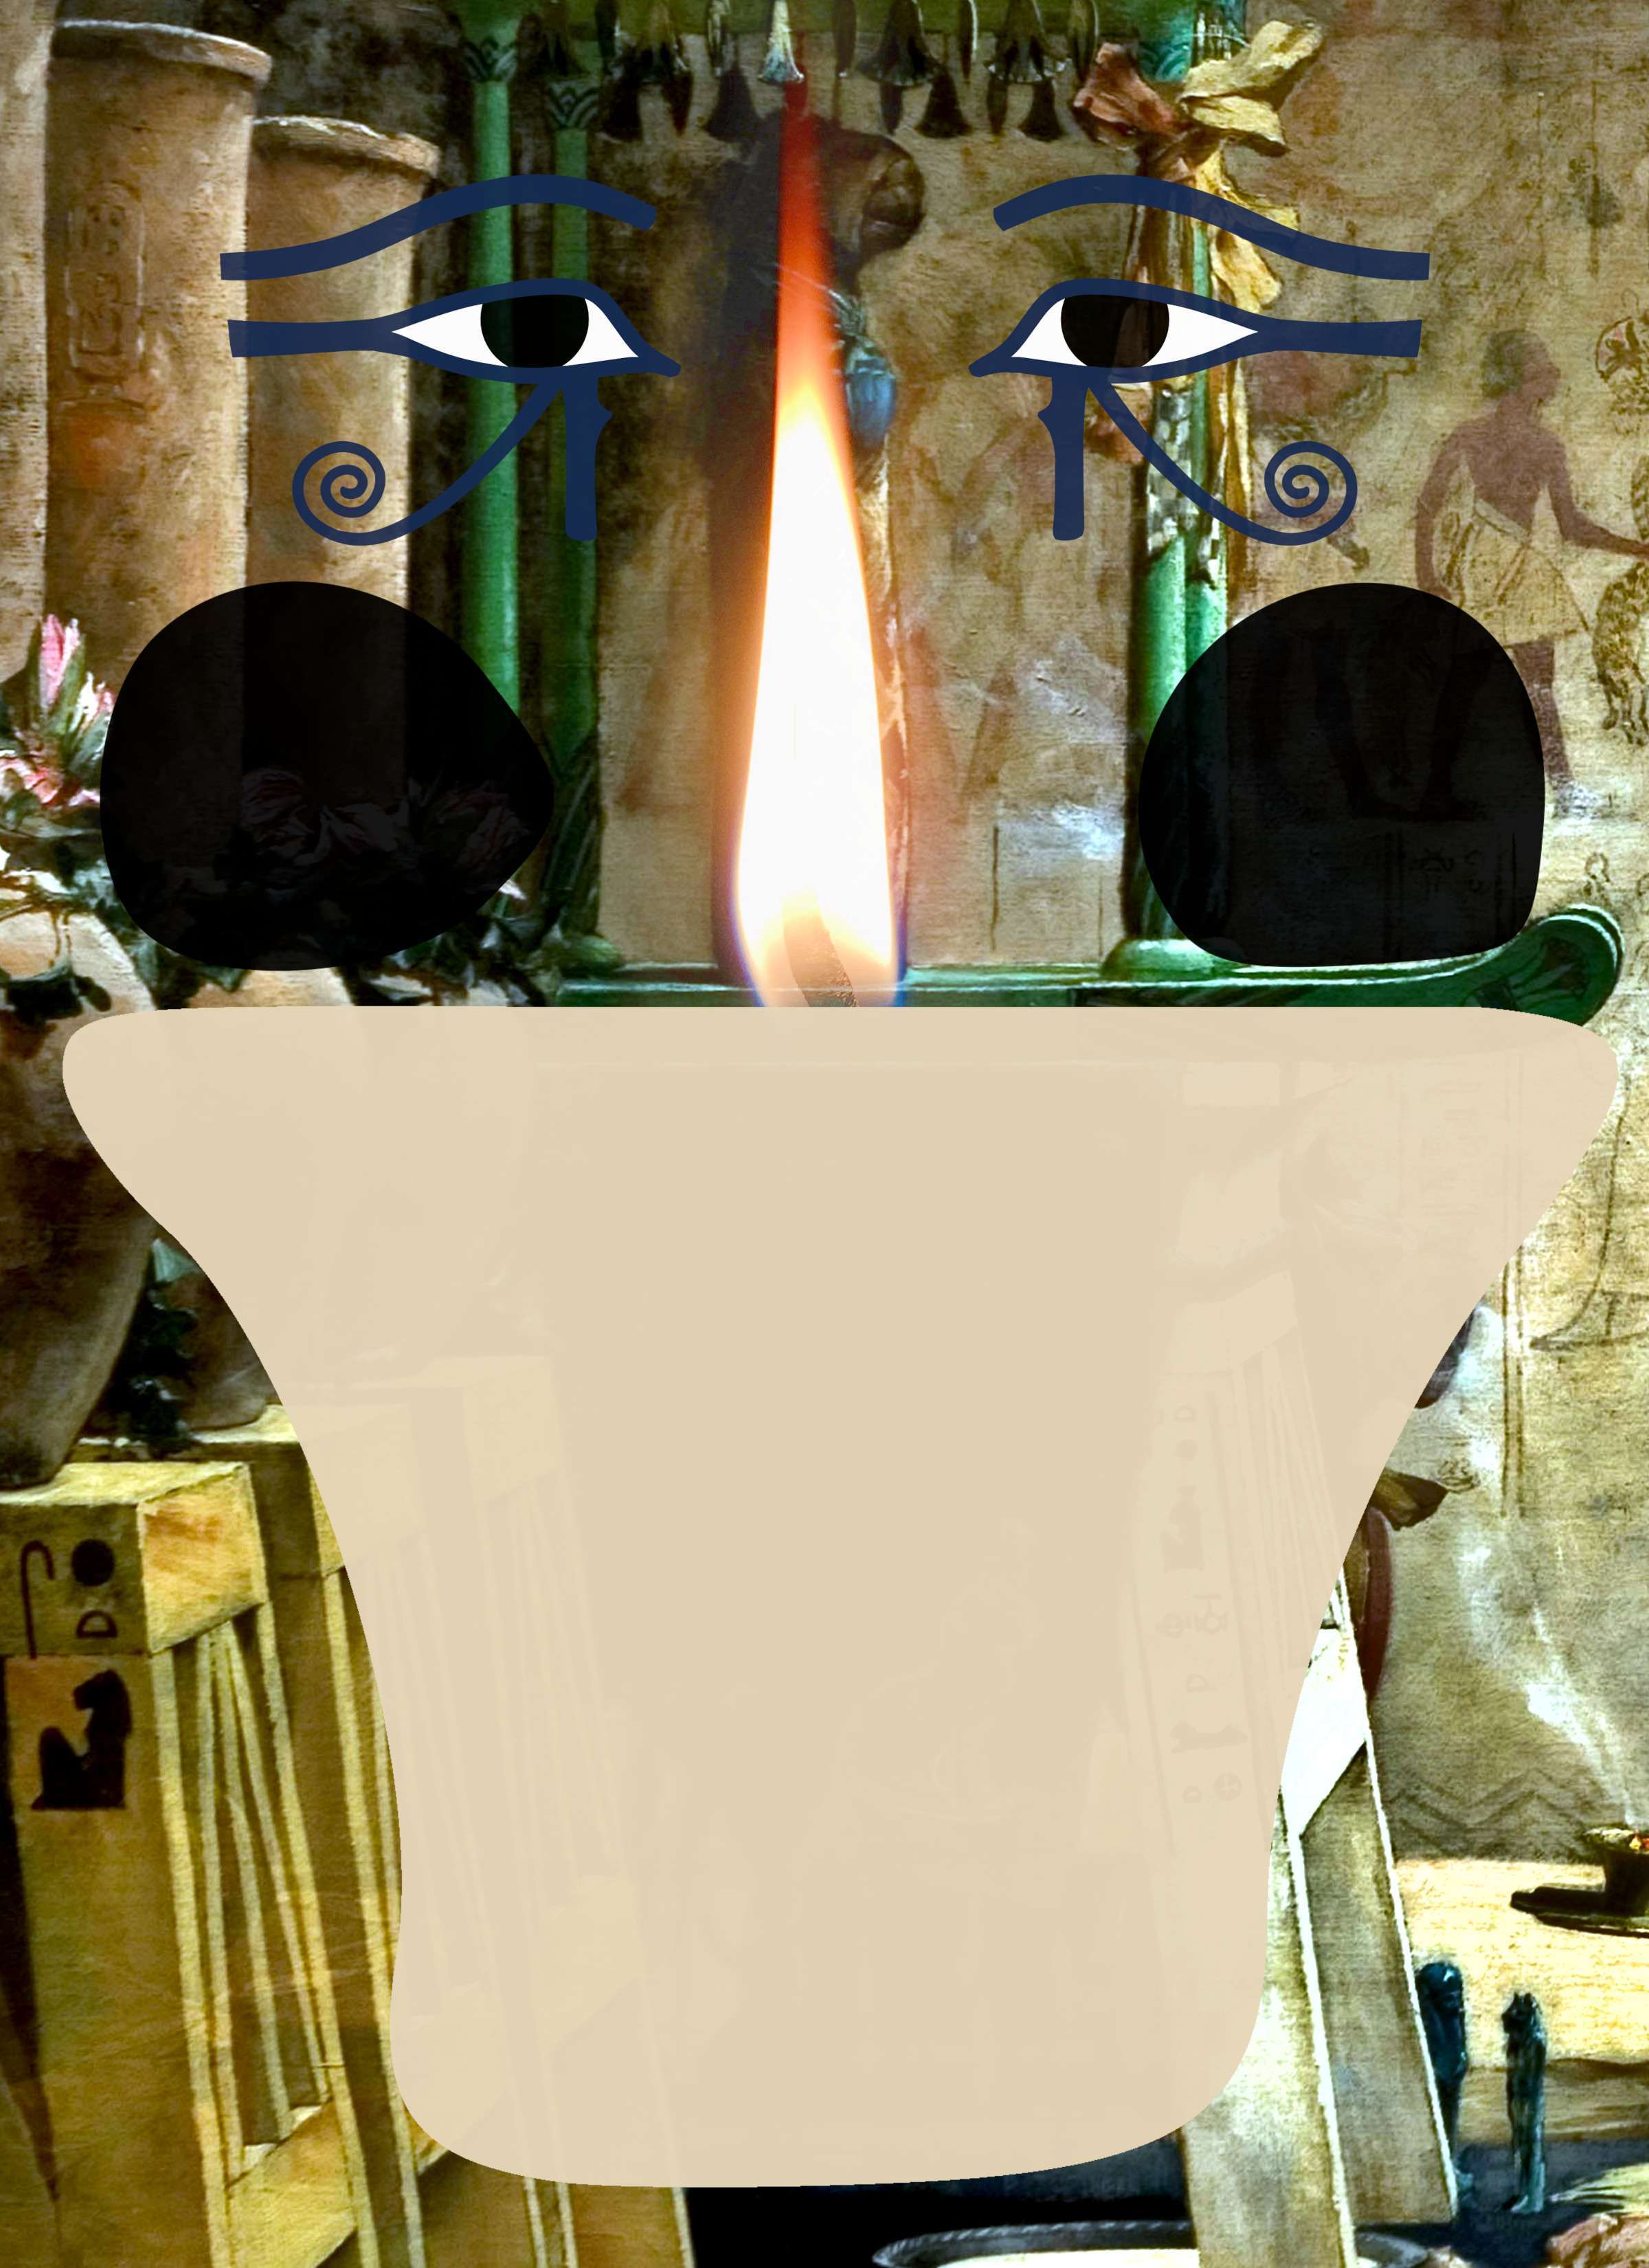
\includegraphics[width=\paperwidth,height=\paperheight]{egyptcustom.jpeg}}
\begin{titlepage} % Suppresses headers and footers on the title page
	\centering % Centre everything on the title page
	%\scshape % Use small caps for all text on the title page

	%------------------------------------------------
	%	Title
	%------------------------------------------------
	
	{\color{myRed}\rule{\textwidth}{1.6pt}\vspace*{-\baselineskip}\vspace*{2pt}} % Thick horizontal rule
	{\color{myRed}\rule{\textwidth}{0.4pt}} % Thin horizontal rule
	
	\vspace{1\baselineskip} % Whitespace above the title

	{\scshape\Huge Le Kyphi}
	
	\vspace{1\baselineskip} % Whitespace above the title

	{\color{myRed}\rule{\textwidth}{0.4pt}\vspace*{-\baselineskip}\vspace{3.2pt}} % Thin horizontal rule
	{\color{myRed}\rule{\textwidth}{1.6pt}} % Thick horizontal rule
	
	\vspace{1\baselineskip} % Whitespace after the title block
	
	%------------------------------------------------
	%	Subtitle
	%------------------------------------------------
	
	{\scshape Parfum sacré des anciens Égyptiens} % Subtitle or further description
	
	\vspace*{1\baselineskip} % Whitespace under the subtitle
	
        {\scshape Par \Large Victor Loret} % Subtitle or further description
    
	%------------------------------------------------
	%	Editor(s)
	%------------------------------------------------
        \vspace*{\fill}

	\vspace{1\baselineskip}

	{\footnotesize\scshape Paris, juillet-août 1887}
	
	{\footnotesize\scshape{Journal Asiatique, Huitième Série --- Tome 10}}
	
	\vspace{0.5\baselineskip} % Whitespace after the title block

        {\footnotesize\scshape Internet Archive Online Edition}  % Publication year
	
	{\scshape\footnotesize Utilisation non commerciale --- Partage dans les mêmes conditions 4.0 International} % Publisher
\end{titlepage}
\setlength{\parskip}{1mm plus1mm minus1mm}
\large
\clearpage
\tableofcontents
\clearpage
\section{}
\paragraph{}
Les auteurs classiques nous ont fait connaître l'existence, chez les anciens Égyptiens, d'un parfum sacré dont ils transcrivent le nom κῦφι. Je réserverai pour un prochain travail l'étude du kyphi au point de vue de son emploi dans le culte égyptien et de son importation dans le monde gréco-romain. Je ne veux aujourd'hui que comparer, aux trois plus anciennes recettes fournies par les auteurs grecs, trois inscriptions d'époque ptolémaïque qui nous enseignent, en hiéroglyphes, la manière de préparer ce parfum.

Les recettes grecques nous ont été transmises par Dioscoride,\footnote{\emph{De materia medica}, 1, 24.} Plutarque\footnote{\emph{De Iside et Osiride}, § 80.} et Galien.\footnote{\emph{De antidotis}, 2, 2.} En voici la traduction :

\bigskip

\begin{center}
\textbf{Dioscoride.}
\end{center}
\paragraph{}
« Le kyphi est un parfum à brûler fort recherché pour le culte, et dont les prêtres égyptiens font le plus grand usage. On le mélange aussi aux antidotes, et on le donne en boisson aux asthmatiques. Il existe plusieurs recettes de ce parfum ; voici l'une d'entre elles : »

« Prenez un demi-setier de cyperus, et la même quantité de baies de genièvre bien grasses ; 12 mines de raisins secs charnus, débarrassés de leurs pépins ; 5 mines de résine purifiée ; calame aromatique, aspalathe, schœnus, 1 mine de chaque ; myrrhe, drachmes; vin vieux, 9 setiers ; miel, 2 mines. »

« Après avoir débarrassé les raisins secs de leurs pépins, hachez-les et broyez-les avec le vin et la myrrhe ; pilez ensuite les autres substances, mélanges-les aux précédentes, et laissez macérer le tout pendant une journée. »

« Faites cuire le miel jusqu'à ce qu'il ait acquis une consistance visqueuse, faites fondre la résine, et mélangez-la soigneusement au miel. Enfin, mêlez le tout ensemble, broyez bien soigneusement, et enfermez dans un vase de terre cuite.\footnote{Éd. C. Sprengel, \emph{Lipsiæ}, 1829.} »

\bigskip

\begin{center}
\textbf{Plutarque.}
\end{center}
\paragraph{}
« Le kyphi est un composé de seize ingrédients : vin, miel, raisins secs, cyperus, résine, myrrhe, aspalathe, séséli, lentisque, asphalte, jonc, patience, les deux espèces de genièvre (que l'on appelle grand et petit genièvre), cardamome et calamus. On ne procède pas sans ordre à ce mélange, mais d'après des formules sacrées qui sont lues aux opérateurs pendant la confection du parfum. Le nombre seize a sa raison d'être : c'est le produit du carré multiplié par lui-même et le seul dont le périmètre soit égal à l'aire ; c'est à cause de cela qu'on l'a choisi ... Les Égyptiens prennent aussi le kyphi en le mélangeant à des boissons, car ils croient que, à cause de ses vertus émollientes, il purge l'intérieur du corps.\footnote{Éd. Dübner, \emph{Parisiis}, 1841.} »

\bigskip

\begin{center}
\textbf{Galien.}
\end{center}
\paragraph{}
« Damocrate fait mention d'un kyphi dont il est l'auteur et il en décrit soigneusement la composition en ces termes : »

« Le kyphi n'est ni un mélange, ni un corps simple ; aucune terre ne le produit, aucune plante ne le laisse écouler après incision. Les Égyptiens, qui le préparent comme je vais dire, le brûlent devant quelques-unes de leurs divinités. »

« Ils prennent des grains de raisins secs bien charnus, puis les dépouillent de leur peau et de leurs pépins. Ils en mesurent 24 drachmes attiques ; même poids de résine de térébenthine brûlée ; myrrhe 12 drachmes, cinnamome 4, schœnus 12 ; safran, 1 drachme ; ongles de bdellium, 3 drachmes ; aspalathe, 2 \emph{semis}, nardostachys 3, bonne cannelle 3 ; cyperus pur, 3 drachmes ; autant de baies de genièvre grosses et grasses, 9 drachmes de calame aromatique, miel en quantité suffisante, vin en faible dose. »

« Ils jettent dans un mortier le bdellium, le vin et la myrrhe, et les broient jusqu'à ce qu'ils aient atteint la consistance d'un miel fluide. Puis ils ajoutent le miel, avec lequel ils ont pilé préalablement les raisins secs. Enfin, ils mêlent toutes les autres substances après les avoir pilées et divisent la masse en petites pastilles rondes, dont ils encensent les dieux. »

« C'est ainsi que Rufus, homme excellent et habile praticien, nous apprend que l'on prépare le kyphi. Quelques-uns, lorsqu'ils n'ont pas de cinnamome à leur disposition, emploient en place des graines de cardamome et les traitent de même. On donne le kyphi à boire, à la dose d'une drachme, à ceux qui souffrent du foie, des poumons, ou des autres parties internes.\footnote{Éd. D. C. Gottlob Kühn, \emph{Lipsiæ}, 1827.} »

Dioscoride n'indique pour le kyphi que onze substances, en considérant, ainsi que le fait Plutarque, les deux espèces de genièvre comme deux substances. Plutarque et Galien en indiquent seize, et l'auteur du traité \emph{Sur Isis et Osiris} insiste sur la raison qui a motivé ce nombre spécial. En fait, les recettes égyptiennes, comme on le verra plus loin, énumèrent effectivement seize ingrédients.

Les recettes grecques ne sont pas identiques. Onze substances seulement se retrouvent dans les trois textes. Ce sont le miel, le vin, les raisins secs, le cyperus, la résine,\footnote{Ῥητίνη, sans épithète, est généralement, et je crois avec raison, considéré comme un synonyme de τερμινθίνη.} la myrrhe, l'aspalathe, les deux espèces de genièvre, le calame et le schœnus, c'est-à-dire justement toutes les substances mentionnées par Dioscoride. Il y a divergence au sujet des cinq autres, à part pourtant pour la cardamome (Plut.), que Galien cite comme pouvant remplacer le cinnamome. Du reste, si mes identifications des noms de plantes pharaoniques sont justes, aucune des deux recettes à seize substances ne se rapporte exactement à la recette égyptienne.

M. G. Parthey, auteur d'une édition du traité de Plutarque, a eu la curiosité de faire exécuter par un pharmacien de Berlin les trois recettes grecques du kyphi. Voici, d'après ce qu'il en dit dans les notes de son édition, l'impression que lui a produite le parfum égyptien :

« Die Versuche mit diesen drei Arten führten zu dem Resultate, dass das Kyphi in kleiner Quantität dem Weine beigemischt, diesem einen sehr adstringenten Geschmack mitteilt, der nur von denen als Wohlgeschmack betrachtet werden dürfte, die sich mit der Herbheit des \emph{Vino resinato} im heutigen Griechenland befreundet haben. Die Mischung 3. (Diosc.) zeigte sich als die beste. »

« Auf ein heisses Blech gestrichen entwickelten alle drei Arten von Kyphi einen scharfen aromatischen keineswegs widerlichen Geruch. Auch hier trug N° 3. den Preis davon.\footnote{G. Parthey, \emph{Über Isis und Osiris, nach neu verglichenen Handschriften mit Übersetzung und Erläuterungen herausgegeben}, Berlin, 1850, p. 277.} »

Si j'ai tenu à rassembler ici les trois principales recettes grecques que nous possédons du kyphi, c'est surtout pour en utiliser les données au point de vue de l'identification de certaines plantes égyptiennes. C'est donc dans l'étude des noms hiéroglyphiques de ces plantes que nous aurons l'occasion d'examiner avec plus de détails les ingrédients mêmes qui entrent dans la composition du parfum.
\clearpage
\section{}
\paragraph{}
Un point reste à éclaircir avant d'entreprendre la traduction des recettes égyptiennes. Quel est le mot hiéroglyphique qui a donné lieu à la transcription κῦφι et quel en est le sens exact ?

D'après toutes les descriptions classiques que nous possédons, le κῦφι est un parfum \emph{à brûler}, θυμίαμα ; c'est là un fait acquis. La composition même du kyphi, --- dans lequel entrent plus de 25 p. \% de résines (myrrhe, lentisque et térébenthine) et presque autant de racines et de bois odoriférants, --- nous prouve qu'il ne pouvait guère en être autrement. Que le kyphi ait été employé à des usages divers par les médecins gréco-latins, cela ne change en rien la destination primitive du parfum égyptien, qui était de servir à encenser les dieux.

Or, un radical égyptien, $\hieroAAAA\:\hieroAAAB\:\hieroAAAC$, $\hieroAAAD$, $\hieroAAAE$, \emph{kap}, a précisément ce sens spécial de « brûler un parfum, » ou mieux, d'une manière plus restreinte et précise, celui de « brûler un corps qui dégage de la fumée sans flammes.\footnote{Un radical \textbf{kap} existe avec le même sens dans les langues indoeuropéennes (P. Regnaud, \emph{Essais de linguistique évolutionniste}, p. 216).} » Ce sens, je crois, n'a jamais été relevé, et il est utile d'en réunir des exemples :

$\hieroAAAF\:\hieroAAAG\:\hieroAAAH\:\hieroAAAI\:\hieroAAAJ\:\hieroAAAA\:\hieroAAAB\:\hieroAAAK\:\hieroAAAL\:\hieroAAAI\:\hieroAAAI\:\hieroAAAI\:\hieroAAAM\:\hieroAAAN$ (Pépi 1, 79) « Il te donne la résine dont sont encensés les dieux ; »

$\hieroAAAA\:\hieroAAAB\:\hieroAAAO\:\hieroAAAP\:\hieroAAAN\:\hieroAAAH\:\hieroAAAQ\:\hieroAAAR$ (Tombe de Hor-hotep, 171, \emph{Miss. da Caire}, 1, 146) « Encenser sa tête avec de la résine ; »

$\hieroAAAA\:\hieroAAAB\:\hieroAAAO\:\hieroAAAS\:\hieroAAAT\:\hieroAAAU\:\hieroAAAY\:\hieroAABI\:\hieroAAAT\:\hieroAAAU\:\hieroAABJ\:\hieroAAAW\:\hieroAAAA\:\hieroAAAB\:\hieroAAAO\:\hieroAAAX\\\hieroAAAY\:\hieroAAAZ\:\hieroAAAT\:\hieroAAAU\:\hieroAAAI\:\hieroAAAH\:\hieroAAAQ\:\hieroAAAX\:\hieroAAAY\:\hieroAAAZ\:\hieroAAAT\:\hieroAAAU$ (\emph{Ib.}, 175) « Horus l'a encensé de son œil : ce défunt Hor-hotep est encensé de l'œil d'Horus, est fumigé\footnote{Remarquer le verbe nouveau \textbf{senter}, « encenser, » en rapport avec \textbf{senter}, « résine. » En voici un second exemple : $\hieroAABA\:\hieroAABB\:\hieroAABC\:\hieroAAAA\:\hieroAAAN\:\hieroAABD\:\hieroAAAB\:\hieroAABB\:\hieroAAAM\:\hieroAABE\:\hieroAAAI\:\hieroAAAH\:\hieroAABF\:\hieroAAAN\:\hieroAABG\:\hieroAAAB\:\hieroAABH$ (Pépi 1, 372), « tu es ablué dans Shé-saba, et encensé dans Taï-t. »} de l'œil d'Horus. »

Ces trois exemples, appartenant aux plus anciens textes, nous fournissent la vocalisation $\hieroAAAB$ du verbe, qu'ils emploient dans le sens spécial de « fumiger (d'une fumée odorante). »

Le mot \textbf{kap} se retrouve plus tard, dans des papyrus médicaux, avec le sens de « fumiger (d'une fumée odorante ou non), fumigation. »

$\hieroAABK\:\hieroAABL\:\hieroAABM\:\hieroAABN\:\hieroAAAT\:\hieroAABO\:\hieroAABP\:\hieroAABQ\:\hieroAAAB\:\hieroAABR\:\hieroAAAM\:\hieroAAAM\:\hieroAABS\:\hieroAABT\:\hieroAABU\:\hieroAABV\:\hieroAABT\:\hieroAABW\:\hieroAAAT\:\hieroAABX$ ... ... $\hieroAABY\:\hieroAABZ\:\hieroAACA\:\hieroAACB\:\hieroAACA\:\hieroAAAU\:\hieroAAAH\:\hieroAACC$ (\emph{Pap. méd. de Berlin}, 7, 6) « Remède pour guérir la piqûre d'un scorpion. Bois épineux, cire, etc. Mettre sur le feu, en fumiger (la personne). »

$\hieroAACB\:\hieroAACA\:\hieroAABL\:\hieroAABM\:\hieroAAAL\:\hieroAACD\:\hieroAACE\:\hieroAACF\:\hieroAACG\:\hieroAACH\:\hieroAACI\:\hieroAABV\:\hieroAABT$ ... ... $\hieroAACB\:\hieroAACA\:\hieroAACJ\:\hieroAAAU\:\hieroAAAH\:\hieroAACC$ (\emph{Pap. méd. de Berlin}, 7, 2) « Fumigation pour guérir les gonflements dans toute maladie. Bois épineux, etc. En fumiger la personne. »

Le même papyrus contient environ une trentaine de recettes analogues,\footnote{Ppl. 5-7.} que je me dispenserai de reproduire, dans lesquelles le mot $\hieroAACB\:\hieroAACA$, $\hieroAAAD\:\hieroAACA$ est employé, dans les titres, avec le sens nominal de « fumigation, » et, dans le corps de la formule, avec le sens verbal de « fumiger. »

$\hieroAABK\:\hieroAACK\:\hieroAACL\:\hieroAACE\:\hieroAACM\:\hieroAACN\:\hieroAACO\:\hieroAACP\:\hieroAACQ\:\hieroAACR\:\hieroAAAI\:\hieroAACS\:\hieroAACT\:\hieroAAAD\:\hieroAACU\:\hieroAACV\:\hieroAACR\\\hieroAAAH\:\hieroAACQ\:\hieroAACW\:\hieroAACX\:\hieroAAAT\:\hieroAACY\:\hieroAACA\:\hieroAAAM\:\hieroAACZ\:\hieroAADA\:\hieroAADB\:\hieroAADC$ (\emph{Pap. Ebers}, 94, 3-5). « Autre [recette pour rétablir la matrice dans sa position normale]. Excréments humains secs. Mêler à de la résine. En fumiger la femme en faisant pénétrer, à l'intérieur de son vagin, la fumée qui s'en dégage. »

Dans ce même traité de médecine, il est fait mention d'un parfum à brûler que des femmes doivent $\hieroAADD\:\hieroAAAN\:\hieroAAAM\:\hieroAADE\:\hieroAAAL\:\hieroAABX\:\hieroAAAD\:\hieroAACA\:\hieroAADF\:\hieroAADG\:\hieroAAAM\:\hieroAAAN\:\hieroAADG$ (98, 12 et sqq), « former en pastilles pour s'en fumiger. »

Ces nombreux exemples nous prouvent d'une manière formelle l'existence d'un verbe actif\footnote{Employé parfois sans complément : $\hieroAACQ\:\hieroAAAN\:\hieroAABZ\:\hieroAACA\:\hieroAACB\:\hieroAACA$ (\emph{Pap. méd. de Berlin}, 6, 3).} $\hieroAAAA\:\hieroAAAB\:\hieroAAAO$, $\hieroAAAD\:\hieroAACA$, \emph{kap}, signifiant « fumiger, encenser, » et d'un substantif $\hieroAACB\:\hieroAACA$ signifiant « fumigation. » 

Un nouveau mot, dérivé du même radical, présente le sens de « parfum à brûler. »

$\hieroAADH\:\hieroAACA\:\hieroAADI\:\hieroAADJ\:\hieroAAAH\:\hieroAADK\:\hieroAAAN\:\hieroAADL\:\hieroAAAH\:\hieroAACY\:\hieroAADM\:\hieroAADN\:\hieroAADO\:\hieroAADP\:\hieroAAAC\:\hieroAAAL$ (\emph{Pap. Ebers}, 98, 12). « Parfum à brûler : choses à faire pour parfumer une habitation ou du linge. »

Ce mot, féminin, devant se lire \emph{kapi} ou \emph{kouphi}, nous donne l'origine de la transcription grecque κῦφι.

Le $\hieroAADH\:\hieroAACA$ du \emph{Papyrus Ebers} est un parfum à brûler quelconque, et la meilleure preuve en est qu'aucun des ingrédients qui le composent ne se retrouve dans les recettes du kyphi que nous analyserons plus loin. D'autres exemples de ce sens général se rencontrent dans des textes ptolémaïques.

$\hieroAADQ\:\hieroAADR\:\hieroAADS\:\hieroAADT\:\hieroAAAR\:\hieroAADU\:\hieroAADV\:\hieroAACA\:\hieroAADW\:\hieroAAAR\:\hieroAADX\:\hieroAAAI\:\hieroAADY\:\hieroAADZ\:\hieroAAEA\:\hieroAAEB$ (Br. et Düm., \emph{Rec.}, 4, 98, 1-2). « Je t'apporte tous les aromates que l'on prépare sous forme de parfums à brûler à l'usage de ton culte. » $\hieroAAEC\:\hieroAAAR\:\hieroAAED\:\hieroAAEE\:\hieroAAAR\:\hieroAAEE\:\hieroAAAR\:\hieroAABV\:\hieroAAEF$ (\emph{Ib.}, 80, h). « Un brûle-parfums avec des parfums à brûler en lui. »

Enfin, une espèce particulière de parfum à brûler est désignée sous la dénomination officielle $\hieroAAAE\:\hieroAAAR\:\hieroAAEG\:\hieroAAEG\:\hieroAAEH\:\hieroAAAI\:\hieroAAEI$ (\emph{Ib.}, 80, e), $\hieroAAAE\:\hieroAAAR\:\hieroAAEJ\:\hieroAAEG\:\hieroAAED\:\hieroAAAI\:\hieroAAEI$ (\emph{Ib.}, 82, 1), $\hieroAAEK\:\hieroAAEL\:\hieroAAEG\:\hieroAAEG\:\hieroAAEM\:\hieroAAAI\:\hieroAAEN\:\hieroAAEO$ (\emph{Ib.}, 84, 1), « parfum à brûler deux fois bon, à l'usage du culte. » C'est ce parfum spécial, dont nous allons étudier les recettes, qui répond au κῦφι des Grecs.

Voici, en résumé, la liste des formes du radical égyptien dont le mot κῦφι n'est que la transcription grecque :

1° $\hieroAAAA\:\hieroAAAB\:\hieroAAAK\:\hieroAAAL$, $\hieroAAAA\:\hieroAAAB\:\hieroAAAO$, $\hieroAACB\:\hieroAACA$, $\hieroAAAD\:\hieroAACA$, $\hieroAAAD\:\hieroAAEP$, \emph{kapou}, « fumiger, encenser ; »

2° $\hieroAACB\:\hieroAACA$, \emph{kapou}, « fumigation ; »

3° $\hieroAADH\:\hieroAACA$, $\hieroAAEE\:\hieroAAAR$, $\hieroAAAE\:\hieroAAAR$, $\hieroAAAE\:\hieroAAEQ$, \emph{koupi-t}, « parfum à brûler, » d'où $\hieroAAEC\:\hieroAAAR\:\hieroAAED\:\hieroAAEE\:\hieroAAAR$, \emph{âkh nou koupi-t}, « brûle-parfums ; »

4° $\hieroAAAE\:\hieroAAAR\:\hieroAAEG\:\hieroAAEG\:\hieroAAED\:\hieroAAAI\:\hieroAAEI$ et variantes, « \emph{Koupi} (\emph{kouphi}) deux fois bon, à l'usage du culte. » Nom officiel du kyphi.

Des trois textes hiéroglyphiques qui nous ont transmis la forme égyptienne de la recette du kyphi, deux se trouvent à Edfou, et le troisième à Philé. Les deux textes d'Edfou, assez différents l'un de l'autre quant à la forme, sont datés du règne de Ptolémée 7, et ont été copiés par M. J. Dümichen.\footnote{Br. et Düm., \emph{Rec.}, 4, 82, 83.} Le texte de Philé, également d'époque ptolémaïque, ne porte aucun nom de souverain. C'est une version presque littérale du premier des deux textes d'Edfou. Il a été publié par Champollion,\footnote{\emph{Not. descript.}, 1, 194.} Brugsch\footnote{Br. et Düm., \emph{Rec.}, 2, 79. Cette copie ne donne que trois colonnes sur six que comporte la recette.} et Dümichen.\footnote{\emph{Ib.}, 4, 84.} J'ai revu moi-même soigneusement ces trois copies lors de mon passage à Philé, et c'est le texte collationné et corrigé que je transcris plus loin.

La recette du kyphi se divise naturellement en cinq sections, qui indiquent autant de phases des manipulations, et que nous traiterons chacune à part pour la commodité et la clarté de l'étude. C'est là un procédé fort utile à employer, qui permet de mieux préciser les détails d'un long texte sans en modifier en rien la forme d'ensemble. Je désigne par \textbf{A} le premier texte d'Edfou,\footnote{\emph{Ib.}, 4, 82.} par \textbf{B} celui de Philé, et par \textbf{C} le second texte d'Edfou.\footnote{\emph{Ib.}, 4, 83.} J'ajouterai enfin que, le commentaire de ces inscriptions étant déjà assez embarrassé par des remarques philologiques et mathématiques, je réserverai pour un chapitre spécial l'identification des divers ingrédients mentionnés dans la recette du kyphi, me contentant, dans la traduction littérale, d'en donner simplement la transcription en lettres françaises.
\clearpage
\section{}
\paragraph{}
Voici, l'une sous l'autre, les rédactions du titre fournies par les textes \textbf{A} et \textbf{B} :

\hspace*{10mm}\textbf{A.}\hspace*{5mm} $\hieroAAER\:\hieroAAES\:\hieroAABT\:\hieroAAET\:\hieroAAAE\:\hieroAAAR\:\hieroAAEJ\:\hieroAAEG\:\hieroAAED\:\hieroAAAI\:\hieroAAEU\:\hieroAAEV\:\hieroAAEI\:\hieroAAEW\:\hieroAABT\:\hieroAAAE\:\hieroAAAR\:\hieroAAEX$

\hspace*{10mm}\textbf{B.}\hspace*{5mm} $\hieroAAEY\:\hieroAAES\:\hieroAADL\:\hieroAAET\:\hieroAAEK\:\hieroAAEL\:\hieroAAEG\:\hieroAAEG\:\hieroAAEM\:\hieroAAAI\:\hieroAAEZ\:\hieroAADL\:\hieroAAEO$

\hspace*{10mm}\textbf{A.}\hspace*{5mm} $\hieroAAFA\:\hieroAABT$

Ces deux textes correspondent exactement l'un à l'autre pour la première partie du titre : \emph{Recette pour faire le kyphi deux fois bon pour les choses divines.} Seul, le texte \textbf{A} donne la suite : \emph{à l'usage des temples} : \emph{kyphi pesant} ten \emph{cent en nombre}. Cette indication de la quantité à obtenir à une grande importance, car nous verrons qu'en effet le poids total du parfum résultant de la préparation se trouve, à quelques grammes près, arriver à cent \emph{ten}. 

Le texte \textbf{C} donne, sous une autre forme, un titre presque analogue, et dans lequel il est également fait mention des cent \emph{ten} :

\hspace*{10mm}\textbf{C.}\hspace*{5mm} $\hieroAAFB\:\hieroAAFC\:\hieroAAES\:\hieroAAET\:\hieroAAAE\:\hieroAAAR\:\hieroAAFD\:\hieroAAFE\:\hieroAAFF\:\hieroAAAM\:\hieroAAAM\:\hieroAAFG\:\hieroAAFH\:\hieroAAFI$

« Autre recette pour faire le kyphi de cent \emph{ten} en sa quantité totale.\footnote{$\hieroAAFH$ me semble être une variante de $\hieroAAHA\:\hieroAAHB$ et désigner la quantité totale « à peu de chose près. » Le poids obtenu, en effet, comme nous le verrons par la suite, n'est pas exactement de cent \emph{ten}, mais de \emph{ten} 100,2.} »

La recette débute par l'énumération de sept substances aromatiques et la spécification de leur poids.

\hspace*{10mm}\textbf{A.}\hspace*{5mm} $\hieroAAFJ\:\hieroAAFK\:\hieroAAFL\:\hieroAAFM$ \hspace*{5mm} $\hieroAACM\:\hieroAAFN\:\hieroAAFO\:\hieroAAFM$ \hspace*{5mm} $\hieroAAFP\:\hieroAAAR\:\hieroAAFM\:$

\hspace*{10mm}\textbf{B.}\hspace*{5mm} $\hieroAAFQ\:\hieroAAFR\:\hieroAAFS\:\hieroAABV\:\hieroAABT\:\hieroAAFT\:\hieroAAFU$ \hspace*{1.3mm} $\hieroAACM\:\hieroAAFV\:\hieroAAFW\:\hieroAAFT\:\hieroAABT$ \hspace*{6.1mm} $\hieroAAFX\:\hieroAAFY\:\hieroAAFT\:\hieroAABT$

\hspace*{10mm}\textbf{A.}\hspace*{5mm} $\hieroAAFZ\:\hieroAAEM\:\hieroAAGA\:\hieroAAHC\:\hieroAABV\:\hieroAAFM$ \hspace*{4.2mm} $\hieroAAGB\:\hieroAAGC\:\hieroAAGD\:\hieroAAFM$ \hspace*{7mm} $\hieroAAGE\:\hieroAAAB\:\hieroAAAM\:\hieroAAAM\:\hieroAAAR\:\hieroAAFM$

\hspace*{10mm}\textbf{B.}\hspace*{5mm} $\hieroAAGF\:\hieroAAGG\:\hieroAAGA\:\hieroAAGH\:\hieroAAFW\:\hieroAAFM$ \hspace*{2.3mm}
$\hieroAAGB\:\hieroAAGC\:\hieroAAAH\:\hieroAAFW\:\hieroAAFT\:\hieroAAGI$ \hspace*{2mm} $\hieroAAGJ\:\hieroAAAB\:\hieroAAAM\:\hieroAAAM\:\hieroAADL\:\hieroAAFM$

\hspace*{10mm}\textbf{A.}\hspace*{5mm} $\hieroAAGK\:\hieroAAGL\:\hieroAAFM$ \hspace*{7.8mm} $\hieroAADU\:\hieroAADS\:\hieroAADT\:\hieroAAAR\:\hieroAAGM$ \hspace*{5.6mm} $\hieroAAGN\:\hieroAAGO\:\hieroAAGP\:\hieroAAGQ\:\hieroAAGR\:\hieroAAGS$

\hspace*{10mm}\textbf{B.}\hspace*{5mm} $\hieroAAGT\:\hieroAAGU\:\hieroAAFM$ \hspace*{8mm} $\hieroAAGV\:\hieroAADS\:\hieroAADT\:\hieroAAAR\:\hieroAAGW$ \hspace*{4.8mm} $\hieroAAGV\:\hieroAAFT\:\hieroAAGX\:\hieroAAGP\:\hieroAAGY\:\hieroAAGZ\:\hieroAAGS$

« 1° \emph{Kanen} ; 2° \emph{Shou-ament} ; 3° \emph{Sheb} ; 4° \emph{Écorce de Qat} ; 5° \emph{Tas} ; 6° \emph{Akaï} ; 7° \emph{Djabâï-t}. Total, sept aromates, faisant, en \emph{ten}, vingt et un. Piler très fin, passer au crible. »

L'identité est complète entre les deux textes, à part au sujet des quantités. Le texte \textbf{A} indique pour chaque substance un poids de 3 \emph{ten}, ce qui donne 7 x 3 = 21. Le texte \textbf{B} indique le même poids pour cinq substances seulement ; la première n'en pèse que 2, et, par compensation, la cinquième en pèse 4, ce qui donne (5 x 3) + 2 + 4 = 21. En somme, le poids total reste le même dans les deux cas.

Le texte \textbf{C} mentionne les sept mêmes substances, mais en les rangeant dans un ordre différent ; de plus, les quantités ne sont pas les mêmes que celles des textes \textbf{A} et \textbf{B}. Enfin, chaque ingrédient est désigné sous deux noms synonymes, ce qui nous sera d'une grande utilité pour les identifications botaniques.

\hspace*{10mm}\textbf{C.}\hspace*{5mm} $\hieroAAHD\:\hieroAAHE\:\hieroAAHF\:\hieroAAHG\:\hieroAAGD\:\hieroAAHH\:\hieroAAHI\:\hieroAAHF\:\hieroAAHG\:\hieroAAGD\:\hieroAAFM\:\hieroAAGA\:\hieroAAHJ\:\hieroAAHK$ \hspace*{5mm} $\hieroAAGB\:\hieroAAGC\:\hieroAAGD\:\hieroAAHH\:\hieroAAHL\:\hieroAADK\:\hieroAADK\:\hieroAABV\:\hieroAAFM\:\hieroAAGA\:\hieroAAHJ\:\hieroAAHK$ \hspace*{5mm} $\hieroAAHM\:\hieroAAGD\:\hieroAAHH\:\hieroAAAH\:\hieroAABB\:\hieroAAFS\:\hieroAAGD\:\hieroAADK\:\hieroAADK\:\hieroAAHN\:\hieroAAGA\:\hieroAAHO$ \hspace*{5mm} $\hieroAACM\:\hieroAAFN\:\hieroAAHP\:\hieroAAHH\:\hieroAAHQ\:\hieroAAFO\:\hieroAAHR\:\hieroAAHS\:\hieroAAHT\:\hieroAAHU\:\hieroAAGA\:\hieroAAHO$ \hspace*{5mm} $\hieroAAGE\:\hieroAAAB\:\hieroAAAM\:\hieroAAAM\:\hieroAABV\:\hieroAAHH\:\hieroAAHV\:\hieroAAHW\:\hieroAAHN\:\hieroAAGA\:\hieroAAHO$ \hspace*{5mm} $\hieroAAHX\:\hieroAAHW\:\hieroAAHH\:\hieroAAHY\:\hieroAAFO\:\hieroAAHN$ \hspace*{5mm} $\hieroAAGK\:\hieroAAGD\:\hieroAAHH\:\hieroAAHZ\:\hieroAAIA\:\hieroAAFO\\\:\hieroAAHN\:\hieroAAIB\:\hieroAADS\:\hieroAADT\:\hieroAAAR\:\hieroAAIC\:\hieroAAID\:\hieroAAIE\:\hieroAAIF\:\hieroAAGA\:\hieroAAIG\:\hieroAAAM\:\hieroAAAL\:\hieroAABT\:\hieroAAIH\:\hieroAAII\:\hieroAAIJ\:\hieroAAIK\:\hieroAAAM\:\hieroAAIL\:\hieroAAIM\:\hieroAAIN$

« 1° Écorce de \emph{Qat}, autrement dit Bois de \emph{Qat} : \emph{ten} 3, \emph{qat} 3 1/3 ; 2° \emph{Tas}, autrement dit Bois odorant : \emph{ten} 3, \emph{qat} 3 1/3 ; 3° \emph{Kanen}, autrement dit Roseau odorant : \emph{ten} 2, \emph{qat} 5 ; 4° \emph{Shou-ament}, autrement dit Jonc d'Éthiopie : \emph{ten} 1, \emph{qat} 5 ; 5° \emph{Akaï}, autrement dit \emph{Nekpet} : \emph{ten} 2, \emph{qat} 5 ; 6° \emph{Sheb}, autrement dit \emph{Fet} : \emph{ten} 2 ; 7° \emph{Djabâï-t}, autrement dit \emph{Djalem}, \emph{ten} 2. Pour les aromates, 7 ; pour les \emph{ten}, 17, 1 2/3. Les mettre dans un mortier et les broyer. »

Cette première section se termine par la division en deux parties de la masse obtenue, la première partie devant être laissée de côté, et la seconde seule devant être utilisée pour la préparation du kyphi.

\hspace*{10mm}\textbf{A.}\hspace*{5mm} $\hieroAACQ\:\hieroAAIO\:\hieroAAIP\:\hieroAAIQ\:\hieroAAIR\:\hieroAAIS\:\hieroAAIT\:\hieroAAIU\:\hieroAAGA\:\hieroAAIV$

\hspace*{10mm}\textbf{B.}\hspace*{5mm} $\hieroAACQ\:\hieroAAIW\:\hieroAAIX\:\hieroAADT\:\hieroAADL\:\hieroAAIP\:\hieroAAIY\:\hieroAAIZ\:\hieroAAAM\:\hieroAAAM\:\hieroAADL$ [$\hieroAABT\:\hieroAAGN\:\hieroAAFT$] $\hieroAAIU\:\hieroAAJA\:\hieroAAJB\:\hieroAAJC$

\hspace*{10mm}\textbf{A.}\hspace*{5mm} $\hieroAAIJ\:\hieroAAJD\:\hieroAAHK\:\hieroAAJE\:\hieroAAGP\:\hieroAAJF\:\hieroAAIT\:\hieroAAJG\:\hieroAAGA\:\hieroAAJH$

\hspace*{10mm}\textbf{B.}\hspace*{5mm} $\hieroAAJI\:\hieroAAJJ\:\hieroAAJK\:\hieroAAGP\:\hieroAAAM\:\hieroAAAM\:\hieroAADL\:\hieroAABT\:\hieroAAGN\:\hieroAAFT\:\hieroAAJL\:\hieroAAGA\:\hieroAAJB\:\hieroAAJH$

« Extraire les 3/5 de la masse (litt. les 1/2 + 1/10) sous forme de \emph{Rohani}, soit \emph{ten} 12, \emph{qat} 6. Enlever les 2/5 qui restent (litt. les 1/3 + 1/15) sous forme de \emph{Nouti}, soit \emph{ten} 8, \emph{qat} 4. »

Le texte \textbf{C} donne les mêmes indications, qui varient naturellement par la quantité, puisque la masse à diviser, au lieu de 21 \emph{ten}, n'en pèse que 17, 1 2/3.

\hspace*{10mm}\textbf{C.}\hspace*{5mm} $\hieroAAJM\:\hieroAAIO\:\hieroAAJN\:\hieroAAJO\:\hieroAAJP\:\hieroAAJQ\:\hieroAAAB\:\hieroAAAM\:\hieroAAAM\:\hieroAAHW\:\hieroAAJR\:\hieroAAJS\:\hieroAAJT\:\hieroAAGA\\\hieroAAJU\:\hieroAAJV\:\hieroAAIG\:\hieroAAJW\:\hieroAAGP\:\hieroAACY\:\hieroAAAM\:\hieroAAAM\:\hieroAAHW\:\hieroAAFD\:\hieroAAJX\:\hieroAAGA\:\hieroAAHJ$

« Extraire de la masse les 2/5 du \emph{Rohaï}\footnote{Remarquer la variante \emph{Rohaï} au lieu de \emph{Rohani}.} qui est en elle, soit \emph{ten} 6, 8 2/3 ; il reste la partie principale, sous forme de \emph{Nouti}, pesant \emph{ten} 10, 3. »

Les trois textes sont bien conformes l'un à l'autre, à part pour les quantités qui, du reste, varieront jusqu'à la fin entre \textbf{A} \textbf{B} et \textbf{C}. La seule différence est que \textbf{A} \textbf{B} ne réserve pour le \emph{Nouti}, et par suite pour le kyphi, que les 2/5 de la masse, tandis que \textbf{C} en réserve les 3/5.

Il reste à examiner, avant de passer à la seconde section, ce qu'est le \emph{Rohani} et ce qu'est le \emph{Nouti}. Le mot $\hieroAAGP\:\hieroAAJF$, $\hieroAAGP\:\hieroAAAM\:\hieroAAAM\:\hieroAADL\:\hieroAABT$, $ \hieroAAGP\:\hieroAACY\:\hieroAAAM\:\hieroAAAM\:\hieroAAHW$, dérivé vraisemblablement de la racine $\hieroAAGP$, « broyer, » que nous avons déjà rencontrée dans notre texte, se rapporte au copte \begin{coptic}noeit\end{coptic}, \begin{coptic}nwit\end{coptic}, \begin{coptic}p\end{coptic}, ἄλευρον, σεμίδαλις, \emph{farina}, \emph{similago}, dérivé, comme $\hieroAAGP\:\hieroAAJF$ de $\hieroAAGP$, du verbe \begin{coptic}nout\end{coptic}, ἀλήθειν, \emph{molere}. Ce serait donc, d'une manière générale, non pas la farine, mais la poudre aromatique résultant du broiement des ingrédients.

On possède de nombreux exemples de $\hieroAAGP\:\hieroAAJF$ dans son sens spécial de « farine » de céréales (froment, orge, sorgho, etc.) ; le sens plus général de « poudre » quelconque est prouvé, en dehors de notre texte, par les différentes phrases citées plus loin, ainsi que par l'expression $\hieroAAGP\:\hieroAACY\:\hieroAAJY\:\hieroAAJZ\:\hieroAAAR$,\footnote{H. Brugsch et J. Dümichen, \emph{Rec. de mon. égypt.}, 4, 89, 11.} qui se rencontre dans une autre recette de parfumerie.

Comme nous le verrons en identifiant les termes botaniques mentionnés dans cette première section, les aromates énumérés jusqu'ici doivent en partie être employés frais pour donner toute leur odeur.

Le mot $\hieroAAGP\:\hieroAAJF$ indique une masse pulvérulente \emph{sèche}, ou relativement sèche ; pour l'obtenir, il fallait donc débarrasser les plantes du suc qu'elles renfermaient, ou au moins d'une grande partie de ce suc. Je crois que le terme \emph{Rohani} désigne justement cette partie liquide des aromates. La façon dont les mots \emph{Nouti} et \emph{Rohani} sont employés, dans ce texte et dans quelques autres, donne une grande vraisemblance à cette manière de voir. Voici trois passages analogues au nôtre, tirés tous trois du temple d'Edfou :

$\hieroAACQ\:\hieroAAIO\:\hieroAAKP\:\hieroAAKQ\:\hieroAAAM\:\hieroAAAM\:\hieroAAAR\:\hieroAAEB\:\hieroAAGN\:\hieroAAKR\:\hieroAAKS\:\hieroAAKT\:\hieroAAKD\:\hieroAAGP\:\hieroAAKU\:\hieroAAKJ\:\hieroAAGN\:\hieroAAKK\:\hieroAAGA\:\hieroAAHO$\footnote{Brugsch et Dümichen, \emph{l. c.}, 93, 30.}

$\hieroAACQ\:\hieroAAIO\:\hieroAAKA\:\hieroAAJQ\:\hieroAAKB\:\hieroAAEB\:\hieroAAGN\:\hieroAAGA\:\hieroAAJU\:\hieroAAIG\:\hieroAAKC\:\hieroAAIG\:\hieroAAKD\:\hieroAAGP\:\hieroAACY\:\hieroAAAR\:\hieroAAJL\:\hieroAAGN\:\hieroAAKK\:\hieroAAGA\:\hieroAABT\:\hieroAAHK$\footnote{\emph{Ib.}, 94, 35.}

$\hieroAACQ\:\hieroAAIO\:\hieroAAKA\:\hieroAAKE$ [$\hieroAAKD$] $\hieroAAIR\:\hieroAAAM\:\hieroAAAM\:\hieroAAAR\:\hieroAAKF\:\hieroAAGA\:\hieroAAKG\:\hieroAAHK\:\hieroAAKC\:\hieroAAJD\:\hieroAAKH\:\hieroAAKI\:\hieroAAGP\:\hieroAACY\:\hieroAAAR\:\hieroAAKJ\:\hieroAAGN\:\hieroAAKK\:\hieroAAGA\:\hieroAAIG$\footnote{\emph{Ib.}, 94, 41.}

« Débarrasser la masse du \emph{Rohani} qui est en elle ; enlever sa poudre première. » Les mots $\hieroAAEB$ indiquent bien que le \emph{Rohani} est une partie constituante des aromates ; le texte \textbf{C} donne également $\hieroAAKL$. De plus, \emph{Nouti} est désigné comme étant la partie principale, $\hieroAAGW\:\hieroAAAC$, des ingrédients, et c'est en effet la seule dont on fasse usage. Tout végétal se compose d'une partie solide et d'une partie liquide. \emph{Nouti} désignant la partie solide, \emph{Rohani} ne peut logiquement désigner que la partie liquide. Ce sens est, d'autre part, rendu presque certain par l'expression $\hieroAAKV$, employée dans le texte \textbf{C} : « après avoir extrait de la masse le \emph{Rohani} qui est en elle, \textbf{il reste} la partie principale, c'est-à-dire le \emph{Nouti} ou poudre. » La partie solide d'un végétal est généralement plus considérable que sa partie liquide ; aussi voyons-nous le texte \textbf{C}, ainsi que les trois autres que nous venons de citer, attribuer au \emph{Rohani} la plus faible partie de la quantité totale, soit 2/5, 1/4, 1/3. En un mot, le texte même de notre recette nous amène à voir dans le \emph{Rohani} le suc des plantes.

Pourtant, en étudiant le mot au point de vue philologique, nous sommes tentés de lui donner un sens moins restreint, d'autant plus qu'il est plus prudent, en ces sortes de recherches, de généraliser un peu que de vouloir trop spécifier. Nous avons relevé six exemples du mot : $\hieroAAIR\:\hieroAAAM\:\hieroAAAM\:\hieroAAAR$ (deux fois), $\hieroAAIR\:\hieroAAAB\:\hieroAAAM\:\hieroAAAM\:\hieroAAHW$, $\hieroAAIR\:\hieroAAKM$, $\hieroAAIR\:\hieroAAIS$ et $\hieroAAIZ\:\hieroAAAM\:\hieroAAAM\:\hieroAAHB$. Nous nous trouvons en présence de deux formes, \emph{Rohaï} et \emph{Rohani}. Mais est-il bien certain que ce soient deux formes ? Le $\hieroAAEH$ de $\hieroAAIR\:\hieroAAKM$ ne pourrait-il, au besoin, être considéré comme un déterminatif, de même que le $\hieroAAEH$ de $\hieroAAIR\:\hieroAAIS$, bien que la lettre $\hieroAAKN$ vienne après ? La forme $\hieroAAIZ\:\hieroAAAM\:\hieroAAAM\:\hieroAAHB$ ne pourrait-elle pas être prise pour une transcription fautive de l'orthographe $\hieroAAIR\:\hieroAAIS$, dans laquelle le $\hieroAAEH$ aurait été envisagé, à tort, comme équivalent de $\hieroAAKO$ ? Il serait étrange de trouver, à la même époque et dans une même localité, deux formes si différentes d'un même mot. D'ailleurs, peu importe que le $\hieroAAKO$ soit fautif ou non, le radical du mot égyptien n'en reste pas moins $\hieroAAIR\:\hieroAAAB\:\hieroAAAM\:\hieroAAAM$.

Un mot copte, \begin{coptic}loih1e\end{coptic}, \begin{coptic}lwih1i\end{coptic}, \begin{coptic}pe\end{coptic}, βόρβορος, ἰλὺς, \emph{lutum}, \emph{limus}, servirait à expliquer notre groupe. $\hieroAAIR\:\hieroAAAM\:\hieroAAAM\:\hieroAAAR$ serait le « résidu bourbeux » du broyage et du criblage, le suc rendu épais par les déchets restés sur le tamis. Ce serait, non la sève pure et limpide, mais la masse humide formée d'une certaine quantité de suc mêlée à la partie grossière des aromates.\footnote{Cf., d'une part, \foreignlanguage{hebrew}{\<lA.ha.h>}, \emph{humectavit}, \foreignlanguage{hebrew}{\<la.h>}, \emph{humidus}, et, d'autre part, $\arabicAAAA$, « enlever l'écorce. »} $\hieroAAGP\:\hieroAAJF\:\hieroAAKJ$ est la masse pulvérulente principale, triée, essentielle ; $\hieroAAIR\:\hieroAAAM\:\hieroAAAM\:\hieroAAAR$ est tout ce qui n'entre pas dans cette masse. Ce sens, plus général que celui de suc, convient d'autant mieux ici que, d'une part, il me paraît impossible d'extraire d'une certaine quantité d'aromates, dont quelques-uns sont ligneux, les 2/3 et même les 3/5 de suc pur, et que, d'autre part, ce suc lui-même constitue souvent la partie la plus odorante d'une plante et ne peut être, par conséquent, rejeté de parti pris.

En résumé, nous traduirons la dernière partie de cette section par : « Enlever de la masse totale, en résidu bourbeux, ses 3/5 ; mettre à part la poudre essentielle qui reste, et qui forme ses 2/5. » Nous verrons plus loin que la poudre essentielle était seule employée dans la confection du kyphi. Cette masse pulvérulente légèrement imprégnée de suc, qui à elle seule constitue jusqu'ici le corps odorant mis en œuvre, s'élève, pour les textes \textbf{A} \textbf{B}, au poids de \emph{ten} 8,4 et, pour le texte \textbf{C}, à celui de \emph{ten} 10,3.
\clearpage
\section{}
\paragraph{}
La seconde section fait intervenir d'abord quatre nouveaux ingrédients, avec l'indication de leur volume en \emph{hin} et de leur poids en \emph{ten}.

\hspace*{10mm}\textbf{A.}\hspace*{5mm} $\hieroAAKW\:\hieroAAAR\:\hieroAAKX$ \hspace*{5mm} $\hieroAAKY\:\hieroAAKZ\:\hieroAAKX$ \hspace*{7.2mm} $\hieroAALA\:\hieroAAAR\:\hieroAAKX$ \hspace*{5mm} $\hieroAALB\:\hieroAAAR\:\hieroAAKX$

\hspace*{10mm}\textbf{B.}\hspace*{5mm} $\hieroAALC\:\hieroAAFO\:\hieroAALD$ \hspace*{6mm} $\hieroAALE\:\hieroAAEH\:\hieroAALF\:\hieroAAGD\:\hieroAABT\:\hieroAAKX$ \hspace*{1mm} $\hieroAALA\:\hieroAAGD\:\hieroAAKX$ \hspace*{5mm} $\hieroAAHX\:\hieroAAFO\:\hieroAAKX$

\hspace*{10mm}\textbf{A.}\hspace*{5mm} $\hieroAALG\:\hieroAAIU$ \hspace*{15mm} $\hieroAAIT\:\hieroAAIU\:\hieroAAGA\:\hieroAAJH$

\hspace*{10mm}\textbf{B.}\hspace*{5mm} $\hieroAALG\:\hieroAAIU\:\hieroAAGN\:\hieroAAFT\:\hieroAAIU\:\hieroAAGN\:\hieroAAFT\:\hieroAAMQ\:\hieroAAGA\:\hieroAALH$

« \emph{Persh}, \emph{Sa(mert)-n-nâl}, \emph{Peqer}, \emph{Sheb} ; chacun 3 \emph{hin}, soit en tout 12 \emph{hin}, pesant 12 \emph{ten}. Total, \emph{ten} 20,4. » Nous réservons l'étude des plantes à plus tard. Nous constaterons seulement qu'un bourdon s'est glissé dans le texte \textbf{A} ; le graveur a confondu $\hieroAALI$ avec $\hieroAALJ$ qui devait venir plus loin et a placé, immédiatement après, le groupe $\hieroAAGA\:\hieroAAJH$. La recette \textbf{B} donne correctement le texte. Ce total de \emph{ten} 20,4 indique la somme des \emph{ten} 8,4 de poudre obtenue dans la première section et des 12 \emph{ten} d'aromates nouveaux énumérés dans la seconde.

L'énumération de ces quatre plantes est plus longuement détaillée dans le texte \textbf{C}. Les noms des deux premières plantes sont accompagnés de synonymes ; de plus, le dernier est différent de \emph{Sheb} et ne peut également en être considéré que comme un équivalent.

\hspace*{10mm}\textbf{C.}\hspace*{5mm} $\hieroAAKW\:\hieroAAHW\:\hieroAAHH\:\hieroAAYS\:\hieroAAAL\:\hieroAAGG\:\hieroAAGD\:\hieroAAYT\:\hieroAAED$ \hspace*{5mm} $\hieroAAKY\:\hieroAAXE\:\hieroAAXB\:\hieroAAHH\:\hieroAAYS\\\hspace*{13mm}\hieroAAXF\:\hieroAAYT\:\hieroAAED$ \hspace*{5mm} $\hieroAALA\:\hieroAAAR\:\hieroAAYT\:\hieroAAED$ \hspace*{5mm} $\hieroAADS\:\hieroAADT\:\hieroAAAR\:\hieroAABT\:\hieroAANQ\:\hieroAANF\:\hieroAAYV\:\hieroAAKK\:\hieroAAYU\:\hieroAAYW\:\hieroAAMY\:\hieroAANF\\\hspace*{13mm}\hieroAAFJ\:\hieroAAAB\:\hieroAAAM\:\hieroAAAM\:\hieroAADT\:\hieroAAXL\:\hieroAAAL\:\hieroAAFZ\:\hieroAAHT\:\hieroAAAM\:\hieroAAYX\:\hieroAADS\:\hieroAALK\:\hieroAADS\:\hieroAALK\:\hieroAALL\:\hieroAAYT\:\hieroAAED\:\hieroAAYY\:\hieroAAGA\:\hieroAAHO\\\hspace*{13mm}\hieroAAYU\:\hieroAAYW\:\hieroAAMY\:\hieroAADJ\:\hieroAADS\:\hieroAADT\:\hieroAAYZ\:\hieroAAAM\:\hieroAAZA\:\hieroAAZB\:\hieroAAGP\:\hieroAAZC\:\hieroAAAM\:\hieroAAAM\:\hieroAAHW\:\hieroAAFD\:\hieroAAJX\:\hieroAAZD\:\hieroAAGA\:\hieroAAHJ$

« \emph{Persh}, autrement dit Grains d'\emph{Uân} : \emph{hin} 2 ; \emph{Sannâr}, autrement dit Graines chevelues : \emph{hin} 2 ; \emph{Peqer} : \emph{hin} 2. Aromates, 6 \emph{hin}. Chaque \emph{hin} pesant 1 \emph{ten}, le poids total est de 6 \emph{ten}. \emph{Qaïoui} d'oasis concassé : \emph{hin} 2. Chaque \emph{hin} de cette substance pesant \emph{ten} 1,5, le poids en est de \emph{ten} 3. Soit, pour les onze aromates réduits en poudre, un poids total de \emph{ten} 19,3. »

Ce texte indique bien que le poids total mentionné à la fin est celui de toutes les substances réunies, qui sont déjà au nombre de 11. La somme, dans le texte \textbf{C}, se décompose ainsi : 10,3 + 6 + 3 = 19,3.

Nous n'avons, jusqu'ici, qu'une masse odorante présentant la forme de poudre. Si, en effet, \textbf{A} \textbf{B} n'indique pas que les quatre nouvelles substances doivent être réduites en poudre, \textbf{C} l'indique bien clairement, d'abord par le mot $\hieroAADS\:\hieroAALK\:\hieroAADS\:\hieroAALK\:\hieroAALL$, s'appliquant spécialement à la dernière substance, ensuite par le mot $\hieroAAGP\:\hieroAACY\:\hieroAAAM\:\hieroAAAM\:\hieroAAHW$ désignant, avant le total général, l'aspect du corps odorant obtenu. Cette poudre va maintenant changer de consistance, grâce à l'intervention du vin, qui en formera une pâte et en augmentera nécessairement le poids.

\hspace*{10mm}\textbf{A.}\hspace*{5mm} $\hieroAALM\:\hieroAALN\:\hieroAALO\:\hieroAAIT\:\hieroAALP$ \hspace*{16mm} $\hieroAAFI\:\hieroAALQ\:\hieroAALR\:\hieroAALS\:\hieroAAAM\:\hieroAAAL$

\hspace*{10mm}\textbf{B.}\hspace*{5mm} $\hieroAALT\:\hieroAAAM\:\hieroAAAM\:\hieroAALU\:\hieroAAAM\:\hieroAALV\:\hieroAALO\:\hieroAAGN\:\hieroAAFT\:\hieroAALP$ \hspace*{2mm} $\hieroAAFI\:\hieroAADL\:\hieroAALW\:\hieroAAAM\:\hieroAALX\:\hieroAAAM\:\hieroAAAL\:\hieroAALY$

\hspace*{10mm}\textbf{A.}\hspace*{5mm} $\hieroAABB\:\hieroAALZ\:\hieroAABE\:\hieroAAMA\:\hieroAAMB\:\hieroAAMC\:\hieroAAMD\:\hieroAAME\:\hieroAAAM\:\hieroAAII\:\hieroAAMF\:\hieroAALI\:\hieroAAGA\:\hieroAAMG$

\hspace*{10mm}\textbf{B.}\hspace*{5mm} $\hieroAAMH\:\hieroAAEM\:\hieroAADS\:\hieroAAAM\:\hieroAAAM\:\hieroAAMI\:\hieroAAAM\:\hieroAAMJ\:\hieroAAMC\:\hieroAAMK\:\hieroAAIW\:\hieroAAAM\:\hieroAALV\:\hieroAALI\:\hieroAAJA\:\hieroAAJB\:\hieroAAML$

\hspace*{10mm}\textbf{A.}\hspace*{5mm} $\hieroAALI\:\hieroAAGA\:\hieroAAHO$ \hspace*{5mm} $\hieroAAMM\:\hieroAAAE\:\hieroAAAR\:\hieroAAAM\:\hieroAAAL\:\hieroAAMN\:\hieroAALJ\:\hieroAAIU\:\hieroAAJV$

\hspace*{10mm}\textbf{B.}\hspace*{5mm} \hspace*{15.4mm} $\hieroAAMM\:\hieroAAEK\:\hieroAAEL\:\hieroAAAM\:\hieroAAMO\:\hieroAALT\:\hieroAAAM\:\hieroAAAM\:\hieroAAMP\:\hieroAAMQ\:\hieroAAIU\:\hieroAAGA\:\hieroAAMR$

« Humecter de vin, 5 \emph{hin}, pesant \emph{ten} 25. La quantité de vin restant liquide après saturation des substances\footnote{Le sens général de cette partie de la phrase est bien évident. Quelques mots nouveaux, ou insuffisamment étudiés jusqu'ici, en rendent néanmoins la traduction littérale peu sûre. Voici celle que je proposerais, sous toute réserve : « La quantité [de vin] qui se perd (\emph{aq}), étant qu'il ne fait point (\emph{au bu ar-f}) entrer dans la masse (\emph{χai}). » La variante $\hieroAANL$ de $\hieroAABB\:\hieroAALZ$ rend incertaine la transcription \emph{bu ar-f} ; d'autre part, le déterminatif $\hieroAADM$, du texte \textbf{C}, semble nous donner un autre mot que $\hieroAADS\:\hieroAAAB\:\hieroAAAM\:\hieroAAAM\:\hieroAANM$, malgré l'orthographe $\hieroAANM$ du texte \textbf{A}.} étant de la moitié, c'est-à-dire \emph{ten} 12,5, il ne se trouve employé que \emph{ten} 12,5 de vin, ce qui donne à la masse imprégnée un poids total de \emph{ten} 32,9. »

Ce poids de ten 32,9 est le résultat des \emph{ten} 12,5 de vin absorbés par les \emph{ten} 20,4 d'ingrédients aromatiques en poudre. On remarquera l'orthographe de basse époque, $\hieroAAMS$, du chiffre 9.

Le texte \textbf{C} donne les mêmes indications, en insistant davantage sur les rapports qui existent entre le volume en \emph{hin} et le poids en \emph{ten} du vin.

\hspace*{10mm}\textbf{C.}\hspace*{5mm} $\hieroAAAM\:\hieroAAIL\:\hieroAAMT\:\hieroAAIL\:\hieroAAMU\:\hieroAALO\:\hieroAAMV\:\hieroAAMW\:\hieroAAMX\:\hieroAAMY\:\hieroAALP\:\hieroAAMZ\:\hieroAALQ\:\hieroAAAM\:\hieroAANA\\\hspace*{13mm}\:\hieroAAAM\:\hieroAAAL\:\hieroAABB\:\hieroAANB\:\hieroAADS\:\hieroAAAM\:\hieroAAAM\:\hieroAADM\:\hieroAALI\:\hieroAAGA\:\hieroAANC\:\hieroAAHC\:\hieroAAAB\:\hieroAAND\:\hieroAAAE\:\hieroAAAR\:\hieroAAAM\:\hieroAAAL\:\hieroAAMN\:\hieroAALJ\:\hieroAANE\:\hieroAAGA\\\hspace*{13mm}\:\hieroAANF\:\hieroAAJV\:\hieroAAAM\:\hieroAAIL\:\hieroAADS\:\hieroAAAB\:\hieroAANG\:\hieroAAIL\:\hieroAANH\:\hieroAAHO\:\hieroAANI\:\hieroAAAM\:\hieroAAAL\:\hieroAANJ\:\hieroAAAM\:\hieroAANK$

« On les humecte de vin, 5 \emph{hin}. Chaque \emph{hin} pesant 5 \emph{ten}, le tout pèse 25 \emph{ten}. La quantité de vin non absorbée par la masse étant de \emph{ten} 12,5, --- la moitié seule du vin s'incorporant au kyphi, --- le poids total de la masse imbibée est de \emph{ten} 31,8 (19,3 + 12,5). On laisse reposer jusqu'au matin, afin que le mélange se tasse.\footnote{Je rapproche ce mot nouveau de $\hieroAAOF\:\hieroAAOG$ « poing, » $\hieroAAOH$ « être étalé, aplati. »} »

Les opérateurs emploient 25 \emph{ten} de vin dont une moitié est perdue et dont l'autre moitié seulement doit s'incorporer à la masse. Puisque toutes les manipulations tendent à un poids général déterminé d'avance, il semblerait plus simple de n'employer que les \emph{ten} 12,5 de vin qui doivent être absorbés par les substances sèches. Le procédé est naïf, mais on le retrouve, sous d'autres formes, dans presque toutes les recettes de parfumerie.
\clearpage
\section{}
\paragraph{}
Le corps obtenu jusqu'ici, se composant d'une poudre mélangée à plus de la moitié de son poids en vin, présente la consistance d'une pâte. Cette nouvelle section introduit deux éléments nouveaux, l'un presque solide, l'autre liquide.

\hspace*{10mm}\textbf{A.}\hspace*{5mm} $\hieroAANN\:\hieroAAAN\:\hieroAANO\:\hieroAANO\:\hieroAANP\:\hieroAANQ\:\hieroAANF\:\hieroAAIG\:\hieroAAIT\:\hieroAAMQ$ \hspace*{7mm} $\hieroAANR\:\hieroAANS\:\hieroAAHC\:\hieroAALO$

\hspace*{10mm}\textbf{B.}\hspace*{5mm} $\hieroAAAM\:\hieroAANT\:\hieroAANU\:\hieroAANV\:\hieroAANW\:\hieroAANQ\:\hieroAANF\:\hieroAAIG\:\hieroAAGN\:\hieroAAFT\:\hieroAAMQ$ \hspace*{5mm} $\hieroAANR\:\hieroAANX\:\hieroAANS\:\hieroAALO$

\hspace*{10mm}\textbf{A.}\hspace*{5mm} $\hieroAAIT\:\hieroAAIU\:\hieroAANY\:\hieroAAIT\:\hieroAAMQ\:\hieroAALP$ \hspace*{8mm} $\hieroAAGP\:\hieroAANZ\:\hieroAAOA\:\hieroAAOB\:\hieroAAOC\:\hieroAAOD\:\hieroAAOE$

\hspace*{10mm}\textbf{B.}\hspace*{5mm} $\hieroAAGN\:\hieroAAFT\:\hieroAALP\:\hieroAAGN\:\hieroAAFT\:\hieroAAMQ\:\hieroAALP$

\hspace*{10mm}\textbf{A.}\hspace*{5mm} $\hieroAAOI\:\hieroAAOJ\:\hieroAAOK\:\hieroAAOL\:\hieroAAIT\:\hieroAAIE\:\hieroAACQ\:\hieroAAIG\:\hieroAAOM\:\hieroAAAE\:\hieroAAAR\:\hieroAAIT\:\hieroAAON\:\hieroAAGN$

\hspace*{10mm}\textbf{B.}\hspace*{5mm} $\hieroAAJI\:\hieroAAEP\:\hieroAAOO\:\hieroAAOP\:\hieroAAAM\:\hieroAAAM\:\hieroAADL\:\hieroAAOQ\:\hieroAANQ\:\hieroAAIE\:\hieroAACQ\:\hieroAAIG\:\hieroAAOR\:\hieroAAOS\:\hieroAAOT\:\hieroAAON$

\hspace*{10mm}\textbf{A.}\hspace*{5mm} $\hieroAAAE\:\hieroAAAR\:\hieroAAOU\:\hieroAAMQ\:\hieroAAIU\:\hieroAAGA\:\hieroAAOV$

\hspace*{10mm}\textbf{B.}\hspace*{5mm} $\hieroAAGN\:\hieroAAAE\:\hieroAAEQ\:\hieroAAFT\:\hieroAAMQ\:\hieroAAMQ\:\hieroAAMQ\:\hieroAAIF\:\hieroAAJA\:\hieroAAJB\:\hieroAAOW$

« \emph{Shep} de Testes, \emph{hin} 6 2/3, pesant \emph{ten} 20, \emph{Arhor} vert, \emph{hin} 5, pesant \emph{ten} 25, ce qui fait en tout \emph{ten} 45. Broyer très fin, enfermer dans un récipient. Enlever le tiers en déchets, soit \emph{ten} 15, et mélanger au kyphi les deux autres tiers, soit \emph{ten} 30, de sorte que le kyphi, en son entier, se trouve atteindre le poids de \emph{ten} 62,9 (= 32,9 + 30). »

Le texte \textbf{C} est beaucoup plus explicite dans cette section et nous permettra de déterminer le sens de quelques groupes douteux des textes \textbf{A} \textbf{B}.

\hspace*{10mm}\textbf{C.}\hspace*{5mm} $\hieroAAOX\:\hieroAAOY\:\hieroAAOZ\:\hieroAAHH\:\hieroAAAM\:\hieroAAPA\:\hieroAAAL\:\hieroAAPB\:\hieroAAHT\:\hieroAAPC\:\hieroAAMV\\\hieroAAFM\:\hieroAAMX\:\hieroAAPD\:\hieroAAFI\:\hieroAAPE\:\hieroAAPF\:\hieroAAPG\:\hieroAACY\:\hieroAAAR\:\hieroAAPH\:\hieroAAPI\:\hieroAAJG$

« \emph{Shep} de Testes, autrement dit Raisins d'oasis, \emph{hin} 4 dont chacun pèse 3 \emph{ten}, ce qui fait 12 \emph{ten} en tout. Cette quantité comprenant un tiers de déchets, soit 4 \emph{ten}, il reste 8 \emph{ten} à employer. »

$\hieroAAPJ\:\hieroAAPK\:\hieroAAGH\:\hieroAAHH\:\hieroAAPL\:\hieroAAAL\:\hieroAAPB\:\hieroAAHT\:\hieroAALO\:\hieroAAMV\:\hieroAAMW\:\hieroAAMX\:\hieroAAMY\:\hieroAALP\:\hieroAALQ\:\hieroAAAM\:\hieroAANA\:\hieroAAPM\:\hieroAAPN\\\hieroAAAC\:\hieroAAAM\:\hieroAAPA\:\hieroAAPO\:\hieroAAED\:\hieroAAPP\:\hieroAAPQ\:\hieroAAPR\:\hieroAAMY\:\hieroAAGI\:\hieroAAGA\:\hieroAAIG\:\hieroAAPI\:\hieroAAMQ\:\hieroAAGA\:\hieroAAJG\:\hieroAAHK$

« \emph{Ar-hor} vert, autrement dit Vin d'oasis, \emph{hin} 5 dont chacun pèse 5 \emph{ten}, ce qui fait 25 \emph{ten} en tout. Ce qui se perd de vin en le mêlant aux raisins étant de \emph{hin} 5/6, soit 1/6 du tout, ou \emph{ten} 4, 1 2/3, il reste à employer \emph{ten} 20,8 1/3. »

$\hieroAAAM\:\hieroAAIL\:\hieroAAPS\:\hieroAAPT\:\hieroAAPU\:\hieroAAPV\:\hieroAAPW\:\hieroAAHH\:\hieroAAPX\:\hieroAAPY\:\hieroAAPZ\:\hieroAAQA\:\hieroAADS\:\hieroAADT\:\hieroAAAR\:\hieroAALQ\:\hieroAAQB\:\hieroAAAE\\\hieroAAAR\:\hieroAALJ\:\hieroAAMQ\:\hieroAAMQ\:\hieroAAGA\:\hieroAANF\:\hieroAAHK\:\hieroAAAM\:\hieroAAIL\:\hieroAADS\:\hieroAAAB\:\hieroAANG\:\hieroAAIL\:\hieroAAQC\:\hieroAANQ\:\hieroAAQD$

« Mettre le tout dans le récipient, autrement dit \emph{Mârekh}, de sorte que les aromates imprégnés pour le kyphi s'élèvent en tout au poids de \emph{ten} 60,6 1/3 (= 31,8 x 8 x 20,8 1/3). --- Les laisser jusqu'au cinquième jour. »

Il nous reste, pour compléter l'étude de cette section, à élucider quelques termes nouveaux.

Le groupe $\hieroAAOC\:\hieroAAOD\:\hieroAAOE$ \textbf{A}, var. $\hieroAAPV\:\hieroAAPW$ \textbf{C}, doit se lire \emph{χnoum our-t}. Le déterminatif représente un récipient circulaire, concave, muni d'un manche. Le synonyme $\hieroAAPX\:\hieroAAPY$ donné par le texte \textbf{C}, semble indiquer que ce récipient est en cuivre, d'abord à cause du déterminatif $\hieroAAQE$, ensuite à cause de son sens radical \begin{coptic}mory\end{coptic}, πυῤῥὸς, \emph{rufus}, \emph{rubicundus}, qui fait allusion à la couleur du métal. Ce récipient devait être de grande dimension, puisqu'il peut contenir près de 63 \emph{ten} de matières, soit un peu moins de 6 kilogrammes. Son nom \emph{χnoum our-t}, « le grand réunisseur, » vient de ses dimensions et de son emploi dans les mélanges de laboratoires ; c'est une sorte de grande bassine en cuivre. Le même mot, du reste, se rencontre dans un texte que j'ai déjà étudié,\footnote{V. Loret, \emph{Les Fêtes d'Osris au mois de Khoïak}, § 93 (\emph{Rec.}, 5, 89).} sous la forme $\hieroAAPV\:\hieroAAQF\:\hieroAAQG$, dans laquelle le manche du récipient se termine par un crochet. Il s'agit, dans ce texte, d'une bassine pouvant contenir au moins 4 litres d'un mélange de terre, encens, myrrhe, etc.

Une nouvelle expression est rendue par trois synonymes, $\hieroAAOK\:\hieroAAOL$, $\hieroAAPG\:\hieroAACY\:\hieroAAAR$ et $\hieroAAQH\:\hieroAAAM\:\hieroAAAM\:\hieroAADL$. Ces mots servent à désigner la partie des raisins secs qu'on ne peut utiliser et que l'on doit jeter ; d'où le sens général « déchets » que je leur ai donné. Les recettes de Dioscoride et de Galien disent qu'avant d'employer les raisins secs, on doit les débarrasser de leurs pépins et de leur peau. $\hieroAAOK\:\hieroAAOL$ peut se rapprocher du copte \begin{coptic}yar\end{coptic}, δορὰ, δέῤῥις, δέρμα, \emph{pellis}, \emph{corium}, et désigner la « peau » du raisin. Je sais que \begin{coptic}yar\end{coptic} a déjà un équivalent en hiéroglyphes sous la forme $\hieroAAQI\:\hieroAABS$, mais ce mot désigne spécialement le « cuir, » la peau d'un animal. $\hieroAAOK\:\hieroAAOL$, déterminé par les trois grains, serait une forme du même mot et désignerait spécialement la « peau » des fruits. $\hieroAAPG\:\hieroAACY\:\hieroAAAR$, dans ce cas,\footnote{Cf. \begin{coptic}kice \=n kim\end{coptic}, $\arabicAAAB$ \emph{granum} (\emph{quod ignoratur}) (\emph{Zeitschr.}, 1886, p. 91), \begin{coptic}kac\end{coptic}, \emph{granulum}, \emph{nucleus fructuum} (A. Peyron, \emph{Lex.}, p. 71).} ne pourrait signifier que « graines, pépins. » Enfin, $\hieroAAQH\:\hieroAAAM\:\hieroAAAM\:\hieroAADL$, dérivé du radical $\hieroAAQH\:\hieroAAQJ$, « débarrasser, délivrer, » désignerait « la partie dont on doit se \emph{débarrasser}, » c'est-à-dire à la fois les pépins et la peau.

Nous devons relever, en dernier lieu, une erreur de gravure qui a fait mettre, dans le texte \textbf{B}, $\hieroAAQK\:\hieroAAQL$ au lieu de $\hieroAAQM$, comme poids des déchets, et l'orthographe curieuse $\hieroAANQ\:\hieroAAQD$, à la fin du texte \textbf{C}, dans laquelle $\hieroAAEH$ est l'indication du nombre ordinal, et $\hieroAAQN\:\hieroAAQO$ une forme inusitée de $\hieroAAQP\:\hieroAAAL\:\hieroAAQQ$.
\clearpage
\section{}
\paragraph{}
La masse obtenue jusqu'ici, dans laquelle entre près de la moitié du poids en vin, pèse \emph{ten} 62,9 pour \textbf{A} \textbf{B}, \emph{ten} 60,6 1/3 pour \textbf{C}, et doit avoir la consistance d'une pâte un peu fluide. La quatrième section introduit d'abord de la résine, ensuite du miel.

\hspace*{10mm}\textbf{A.}\hspace*{5mm} $\hieroAAQR\:\hieroAAQS\:\hieroAAGA\:\hieroAABT\:\hieroAAHK$ \hspace*{11mm} $\hieroAAQT\:\hieroAANQ\:\hieroAANF\:\hieroAAIG\:\hieroAAIT\:\hieroAAMQ\:\hieroAANY\:\hieroAAGA\:\hieroAABT\:\hieroAAHK$

\hspace*{10mm}\textbf{B.}\hspace*{5mm} $\hieroAAQR\:\hieroAAFT\:\hieroAANY\:\hieroAAGA\:\hieroAAJB\:\hieroAAHJ\:\hieroAAHK$ \hspace*{3mm} $\hieroAANR\:\hieroAAQU\:\hieroAAQV\:\hieroAANQ\:\hieroAANF\:\hieroAAIG\:\hieroAAQW\:\hieroAAGA\:\hieroAAJB\:\hieroAABT\:\hieroAABT\:\hieroAAJV\:\hieroAAHK$

\hspace*{10mm}\textbf{A.}\hspace*{5mm} $\hieroAAIT\:\hieroAAMQ\:\hieroAAMQ\:\hieroAANF\:\hieroAAGA\:\hieroAAJU\:\hieroAAIG$

\hspace*{10mm}\textbf{B.}\hspace*{5mm} $\hieroAALG\:\hieroAAMQ\:\hieroAAMQ\:\hieroAANF\:\hieroAAGA\:\hieroAAJB\:\hieroAAJU\:\hieroAAIG$

« Résine, \emph{ten} 13,3 1/3. Miel, \emph{hin} 6 2/3, pesant \emph{ten} 33,3 1/5. Soit, en tout : résine et miel, \emph{ten} 46,6 2/3. »

Le texte \textbf{B} contient deux erreurs, faciles à corriger. Au lieu de « \emph{ten} 33,3 1/3, » il porte « \emph{hin} 3,8 1/3, » indication évidemment fautive. De plus, on retrouve le mot $\hieroAAQN\:\hieroAAEH$ employé à tort pour $\hieroAAHU$, faute que nous avons déjà eu l'occasion de relever, pour le même texte, dans la troisième section.

\hspace*{10mm}\textbf{A.}\hspace*{5mm} $\hieroAAQX\:\hieroAAPB\:\hieroAAFJ\:\hieroAAAC\:\hieroAAAH\:\hieroAACA\:\hieroAAAN\:\hieroAAIG\:\hieroAAQY\:\hieroAACA\:\hieroAAQZ\:\hieroAAKD\:\hieroAARA\:\hieroAARB\:\hieroAARC\:\hieroAARD\:\hieroAACA$

\hspace*{10mm}\textbf{B.}\hspace*{5mm} $\hieroAACQ\:\hieroAARE\:\hieroAARF\:\hieroAARG\:\hieroAAAC\:\hieroAAAH\:\hieroAACA\:\hieroAARH\:\hieroAAIG\:\hieroAARI\:\hieroAACA\:\hieroAAKD\:\hieroAARJ\:\hieroAARB\:\hieroAARC\:\hieroAARD\:\hieroAACA$

\hspace*{10mm}\textbf{A.}\hspace*{5mm} $\hieroAAIT\:\hieroAAGM\:\hieroAAIF\:\hieroAAGA\:\hieroAABT\:\hieroAAHK\:\hieroAAPI\:\hieroAAMQ\:\hieroAAIE\:\hieroAAIF\:\hieroAAGA\:\hieroAABT\:\hieroAAHK$

\hspace*{10mm}\textbf{B.}\hspace*{5mm} ...

« Mettre dans une marmite. Cuire jusqu'à un degré d'épaississement\footnote{Litt. « à un tiers d'épaississement. » $\hieroAARI\:\hieroAACA$, écrit $\hieroAARK$ dans le texte \textbf{C}, paraît dériver du radical $\hieroAAAH\:\hieroAARL\:\hieroAALR\:\hieroAARM$, $\hieroAAAH\:\hieroAARN$, lequel a comme sens premier celui de « resserrer, contracter. » De \emph{contracter} à \emph{épaissir} la nuance est presque insaisissable : une masse qui se contracte s'épaissit nécessairement, en ce sens qu'elle présente dans un espace donné un plus grand nombre de molécules. Du reste, le sens « épaissir » est prouvé par un certain nombre d'exemples. Dans un tombeau de Béni-Hassan (Ch., \emph{Not. descr.}, 2, 371), des personnages qui renforcent la pâte en y versant de la farine sont accompagnés de la légende $\hieroAAAH\:\hieroAARN\:\hieroAACA\:\hieroAADS\:\hieroAAAB\:\hieroAARO$, $\hieroAAAH\:\hieroAARP\:\hieroAADS\:\hieroAARO$, « épaissir la pâte. » La phrase suivante précise encore mieux le sens : $\hieroAARX\:\hieroAARQ\:\hieroAARR\:\hieroAARS\:\hieroAART\:\hieroAARU\:\hieroAADF\:\hieroAARV\:\hieroAARW\:\hieroAAAR\:\hieroAARX\:\hieroAARQ\:\hieroAARY\:\hieroAAAM\:\hieroAAAL\:\hieroAARZ\:\hieroAASA\:\hieroAAAN\:\hieroAAAN\:\hieroAADF\:\hieroAASB\:\hieroAAAN\:\hieroAAGB\:\hieroAASC\:\hieroAAEH\:\hieroAADK\:\hieroAADK$ (Br. et Düm., \emph{Rec.}, 4, 97, 16), « Si tu trouves (cet onguent) trop mou, tu l'épaissis avec de l'encens ; si tu le trouves trop dur, tu l'éclaircis avec de l'essence de styrax. » Enfin, on trouve le même mot dans cette expression : $\hieroAAAI\:\hieroAACS\:\hieroAASD\:\hieroAAAM\:\hieroAASE\:\hieroAAHW\:\hieroAAAH\:\hieroAASX\:\hieroAASY\:\hieroAACA$ (\emph{Gr. Pap. Harris}, 1, 18, 6). $\hieroAAAI\:\hieroAACS\:\hieroAASD\:\hieroAAAM\:\hieroAASE\:\hieroAAHW\:\hieroAAAH\:\hieroAARL\:\hieroAALR\:\hieroAARM\:\hieroAACA$ (\emph{Pap. médic. de Londres}, fragm. 2, p. 1, l. 3), où il désigne une résine épaisse, sèche, par opposition à la résine fraîche, $\hieroAANS$. Un nouveau mot est donc à ajouter au dictionnaire : \textbf{saq}, déterminé par $\hieroAACA$, « épaissir (au feu, par évaporation). »} tel, que la quantité perdue au feu soit de 1/5 du poids, ou \emph{ten} 9,3 1/3, de sorte qu'il reste \emph{ten} 37,3 1/3. »

Ces poids sont parfaitement justes ; en effet, 46,6 2/3 - 9,3 1/3 = 37,3 1/3. Le texte \textbf{B} s'interrompt brusquement par suite d'un bourdon ; $\hieroAARB\:\hieroAARC\:\hieroAAEI\:\hieroAACA$ revient en effet dans la phrase suivante, et le graveur a passé tout l'ensemble de signes compris entre ces deux $\hieroAARB\:\hieroAARC\:\hieroAAEI\:\hieroAACA$. 

\hspace*{10mm}\textbf{A.}\hspace*{5mm} $\hieroAACQ\:\hieroAAAE\:\hieroAAAR\:\hieroAAOU\:\hieroAAMQ\:\hieroAAMQ\:\hieroAAGA\:\hieroAAJU\:\hieroAAHJ\:\hieroAACR\:\hieroAASF\:\hieroAAAH\:\hieroAACA\:\hieroAAQZ\:\hieroAASG\:\hieroAASH\:\hieroAASI\:\hieroAARB\:\hieroAARC\:\hieroAAEI\:\hieroAACA$

\hspace*{10mm}\textbf{B.}\hspace*{5mm} ...

\hspace*{10mm}\textbf{A.}\hspace*{5mm} $\hieroAAIT\:\hieroAAIU\:\hieroAAGA\:\hieroAAGI\:\hieroAAJV\:\hieroAAPI\:\hieroAASJ\:\hieroAAGA\:\hieroAAHJ$ \hspace*{22mm} $\hieroAAGN\:\hieroAAAE\:\hieroAAAR\:\hieroAALJ$

\hspace*{10mm}\textbf{B.}\hspace*{5mm} $\hieroAAGN\:\hieroAAFT\:\hieroAAIU\:\hieroAAGA\:\hieroAAJB\:\hieroAASK\:\hieroAAGN\:\hieroAAFT\:\hieroAASJ\:\hieroAAGA\:\hieroAAJB\:\hieroAAHJ\:$ \hspace*{8mm} $\hieroAAGN\:\hieroAAEK\:\hieroAASL$

\hspace*{10mm}\textbf{A.}\hspace*{5mm} $\hieroAASM\:\hieroAAGM\:\hieroAAGA\:\hieroAAJU\:\hieroAAHK$

\hspace*{10mm}\textbf{B.}\hspace*{5mm} $\hieroAASM\:\hieroAAGI\:\hieroAAHJ\:\hieroAAGA\:\hieroAAJB\:\hieroAAGI\:\hieroAAJV\:\hieroAAIG\:\hieroAAHK$

« Prendre les \emph{ten} 62,9 de kyphi et les cuire jusqu'à ce que 1/5 du poids se perde au feu, soit \emph{ten} 12,6, de sorte qu'il reste \emph{ten} 50,3. Le poids total du parfum est alors de \emph{ten} 87,6 1/3 (kyphi 50,3 + résine et miel 37,3 1/3). »

Il y a dans cette opération une légère erreur de calcul, reproduite dans les deux recettes \textbf{A} \textbf{B}. Le 1/5 de 62,9 est 12,5 4/5, et non pas 12,6 comme l'indique le texte. Toute la suite des indications mathématiques nous prouve que l'erreur vient de l'auteur de la recette, et non du graveur. D'autre part, le texte \textbf{B} porte à tort, avant le $\hieroAAHK$ final, un signe $\hieroAAIG$ qui n'a que faire dans la phrase et qui est évidemment à supprimer.

Le texte \textbf{C} est, dans cette section, un peu moins explicite que les textes \textbf{A} \textbf{B}, sans lesquels on pourrait à peine le comprendre. L'emploi du feu et la perte résultant de l'évaporation n'y sont, entre autres, que fort sommairement indiqués.

\hspace*{10mm}\textbf{C.}\hspace*{5mm} $\hieroAAQR\:\hieroAAPK\:\hieroAASO\:\hieroAAAM\:\hieroAASZ\:\hieroAASP\:\hieroAASQ\:\hieroAARK\:\hieroAACC\:\hieroAASR\:\hieroAAQZ\:\hieroAAHU\:\hieroAAGA\:\hieroAASS\\\hieroAAST\:\hieroAASU\:\hieroAAEM\:\hieroAASV\:\hieroAAPI\:\hieroAAGA\:\hieroAASW$

« Résine fraîche, \emph{ten} 10. On la fait épaissir au feu de telle sorte que la perte produite par l'évaporation soit de \emph{ten} 1,1 1/9, [soit 1/9 du poids total. Reste \emph{ten} 8,8 8/9]. »

La fin de cette phrase est complètement fautive. Il faut restituer, comme le prouvent le calcul des quantités et la suite du texte, la formule suivante après $\hieroAAST$ : [$\hieroAATA\:\hieroAAIF\:\hieroAAEM\:\hieroAASV\:\hieroAAPI\:\hieroAAJG\:\hieroAAGA\:\hieroAANF\:\hieroAAJV\:\hieroAAIG\:\hieroAAPR\:\hieroAATB$].

\hspace*{10mm}\textbf{C.}\hspace*{5mm} $\hieroAATC\:\hieroAAEH\:\hieroAALO\:\hieroAAMV\:\hieroAALI\:\hieroAAGA\:\hieroAANC\:\hieroAATD\:\hieroAAMY\:\hieroAAMQ\:\hieroAAIE\:\hieroAAIF\:\hieroAAGA\:\hieroAAHO\:\hieroAAFI\:\hieroAAPQ\:\hieroAAKE\:\hieroAAIF\\\:\hieroAATE\:\hieroAABN\:\hieroAACA\:\hieroAATF\:\hieroAAGA\:\hieroAATG\:\hieroAAPI\:\hieroAAMQ\:\hieroAANE\:\hieroAAGA\:\hieroAABT\:\hieroAAKH$

« Miel, \emph{hin} 5. Chaque \emph{hin} pesant \emph{ten} 7.5, le poids total est de \emph{ten} 37,5. La quantité qui se perd à la cuisson étant de 1/6, soit \emph{ten} 6,2 1/2, il reste \emph{ten} 31,2 1/2. »

Encore une erreur de chiffres à signaler. Les derniers signes, d'après le calcul, doivent se lire $\hieroAAGA\:\hieroAAIF\:\hieroAAKH$.

\hspace*{10mm}\textbf{C.}\hspace*{5mm} $\hieroAAAM\:\hieroAASZ\:\hieroAATH\:\hieroAAAE\:\hieroAAAR\:\hieroAALQ\:\hieroAATI\:\hieroAAPZ\:\hieroAASZ\:\hieroAAMY\:\hieroAAQV\:\hieroAAGA\:\hieroAAGM\:\hieroAATJ\:\hieroAAFI\:\hieroAAPQ\:\hieroAATL$ \\\hspace*{10mm} $\hieroAATM\:\hieroAASO\:\hieroAATJ\:\hieroAAPI\:\hieroAASM\:\hieroAATN\:\hieroAAGA\:\hieroAAGM\:\hieroAAAM\:\hieroAASZ\:\hieroAADS\:\hieroAAAB\:\hieroAANG\:\hieroAASZ\:\hieroAATK\:\hieroAAHO\:\hieroAANI$

« Ajouter à ces deux substances le kyphi imbibé de vin, ce qui fait en tout \emph{ten} 100,7 13/18. La quantité de kyphi évaporée au feu étant de 1/10 du poids, soit \emph{ten} 10 13/18, il reste en tout \emph{ten} 90,7. Le laisser reposer jusqu'au lendemain matin. »

La somme 100,7 13/18 est le résultat de kyphi 60,6 1/3 + résine 8,8 8/9 + miel 31,2 1/2. On doit remarquer l'expression fractionnaire $\hieroAATO$ qui, d'après les calculs, ne peut signifier que 12/18. Il faut peut-être y voir une transcription de l'hiératique $\hieroAATP$ qui signifie 1/4 + 1/2 c'est-à-dire 13,5/18. Dans ce cas il y aurait, dans les calculs de l'auteur, une erreur de 1,5/18. Ce même $\hieroAATO$ revenant dans l'expression \emph{ten} 10 13/18 est du reste encore une erreur de calcul. Le 1/10 de \emph{ten} 100,7 13/18 serait en effet 10 139/180 et non 10 13/18.
\clearpage
\section{}
\paragraph{}
Le parfum obtenu pèse maintenant \emph{ten} 87,6 1/3 pour \textbf{A} \textbf{B}, et \emph{ten} 90,7 pour \textbf{C}. La recette s'achève en quelques mots par l'indication d'une certaine quantité de myrrhe à ajouter à la masse.

\hspace*{10mm}\textbf{A.}\hspace*{5mm} $\hieroAADF\:\hieroAAAR\:\hieroAATQ\:\hieroAATR\:\hieroAAJD\:\hieroAATL\:\hieroAATS\:\hieroAATS\:\hieroAASM\:\hieroAAIT\:\hieroAAIU\:\hieroAAGA\:\hieroAAGM\:\hieroAAIT\:\hieroAAQV\:\hieroAAGA\:\hieroAABT$

\hspace*{10mm}\textbf{B.}\hspace*{5mm} $\hieroAADS\:\hieroAATT\:\hieroAATQ\:\hieroAATU\:\hieroAAIW\:\hieroAATV\:\hieroAATW\:\hieroAATX\:\hieroAATY\:\hieroAATZ\:\hieroAAIT\:\hieroAAIU\:\hieroAAGA\:\hieroAAJB\:\hieroAAUA\:\hieroAAGN$

\hspace*{10mm}\textbf{A.}\hspace*{5mm} $\hieroAAHK\:\hieroAAAE\:\hieroAAAR\:\hieroAAEG\:\hieroAAEG\:\hieroAAAC\:\hieroAAAL\:\hieroAAUB\:\hieroAAEB$

\hspace*{10mm}\textbf{B.}\hspace*{5mm} $\hieroAAFT\:\hieroAAQV\:\hieroAAGA\:\hieroAAJB\:\hieroAAHJ\:\hieroAAHK\:\hieroAAEK\:\hieroAAUC\:\hieroAAUD\:\hieroAAUE\:\hieroAAUF$

« Myrrhe de troisième qualité, 13/90 du poids de la masse, soit \emph{ten} 12,7 ; ce qui porte au poids de \emph{ten} 100,3 1/3 la quantité du kyphi deux fois bon à l'usage du culte. »

Comme on le voit, le résultat final des opérations dépasse légèrement la quantité de 100 \emph{ten} indiquée dans le titre. Du reste il y a encore ici une petite erreur de calcul ; les 13/90 de 87,6 1/3 ne sont 12,7 qu'à 2/45 près. Les mots \emph{ar χet am-f} manquent dans le texte \textbf{B}.

La recette \textbf{C} est un peu plus étendue dans cette dernière partie ; elle fait mention d'un point important, à savoir qu'il faut broyer et tamiser la myrrhe.

\hspace*{10mm}\textbf{C.}\hspace*{5mm} $\hieroAAUG\:\hieroAADF\:\hieroAAAM\:\hieroAAAM\:\hieroAAAR\:\hieroAASO\:\hieroAAFI\:\hieroAAHC\:\hieroAAAB\:\hieroAAUH\:\hieroAAQZ\:\hieroAAUI\:\hieroAAIM\:\hieroAAUJ\:\hieroAAGS\:\hieroAAPQ$ \\\hspace*{10mm} $\hieroAAUK\:\hieroAAGA\:\hieroAAJB\:\hieroAAUL\:\hieroAARL\:\hieroAASZ\:\hieroAAUM\:\hieroAAGA\:\hieroAAJB\:\hieroAAHO\:\hieroAAEB\:\hieroAAII\:\hieroAAAE\:\hieroAAAR\:\hieroAAUN\:\hieroAASM\:\hieroAAGA\:\hieroAAJG\:\hieroAAUO\:\hieroAAAR$ \\\hspace*{10mm} $\hieroAAUP\:\hieroAAGA\:\hieroAAJV$

« Ajouter myrrhe, 10 \emph{ten}. La perte résultant du broyage et du criblage étant de 1/20 de la quantité, soit \emph{ten} 0,5, il reste \emph{ten} 9,5 qui, ajoutés aux \emph{ten} 90,7 de parfum déjà obtenu, font, en tout, pour le kyphi, un poids de \emph{ten} 100,2. »

Il y a dans ce texte une erreur manifeste. Au lieu de $\hieroAAUN\:\hieroAAMQ\:\hieroAAMQ\:\hieroAAMQ\:\hieroAAGA\:\hieroAAJG$, il faut lire $\hieroAAOU\:\hieroAAMQ\:\hieroAAMQ\:\hieroAAMQ\:\hieroAAGA\:\hieroAAGM$, chiffres d'autant plus certains qu'ils sont déjà indiqués dans la section précédente. Le kyphi \textbf{A} \textbf{B} dépasse cent \emph{ten} de 0,3 1/3 ; le kyphi \textbf{C} ne les dépasse, comme on le voit, que de 0,2.
\clearpage
\section{}
\paragraph{}
Il me reste, pour compléter l'étude de la recette égyptienne du kyphi, à en déterminer la partie la plus spéciale et la plus intéressante, c'est-à-dire à identifier les différents ingrédients qui entrent dans la composition de ce parfum sacré. Je les étudierai tour à tour, selon l'ordre dans lequel ils se présentent au cours du texte hiéroglyphique.

1. $\hieroAAFJ\:\hieroAAFK\:\hieroAAFL$, $\hieroAAFQ\:\hieroAAFR\:\hieroAAFS\:\hieroAABV\:\hieroAABT$, $\hieroAAHM\:\hieroAAUQ\:\hieroAAHH\:\hieroAAAH\:\hieroAABB\:\hieroAAFS\:\hieroAAUQ\:\hieroAADK\:\hieroAADK$. J'ai déjà étudié ce groupe par ailleurs\footnote{\emph{Rec.}, 1, 190, 4, 156.} et je suis arrivé, à la suite de recherches qu'il serait superflu de reproduire ici, à montrer qu'il désigne le \emph{Calamus aromaticus} des anciens, soit notre \emph{Acorus Calamus} L. Cette plante est du reste rangée par les auteurs grecs, sous le nom de κάλαμος, au nombre des ingrédients du kyphi. Aux équivalents hébreux de $\hieroAAHM\:\hieroAAUQ$ que j'ai cités dans une précédente étude, j'ajouterai l'équivalent arabe $\arabicAAAC$, qui a le même sens \emph{canna}, \emph{calamus}.

2. $\hieroAACM\:\hieroAAFN\:\hieroAAFO$, $\hieroAACM\:\hieroAAFV\:\hieroAAFW$, $\hieroAACM\:\hieroAAFN\:\hieroAAUR\:\hieroAAHH\:\hieroAAHQ\:\hieroAAFO\:\hieroAAUS\:\hieroAAHS\:\hieroAAHT$. La seconde variante de ce mot, $\hieroAACM\:\hieroAAFV\:\hieroAAFW$, a été copiée de différentes manières. M. Brugsch lit $\hieroAAHF$ comme second signe,\footnote{Br. et Düm., \emph{Rec.}, 2, 79, 2.} M. Dümichen lit $\hieroAAUT$,\footnote{\emph{Ibid.}, 4, 84.} et Champollion $\hieroAAUU$.\footnote{\emph{Not. descript.}, 1, 194.} J'ai revu moi-même soigneusement le texte à Philé, et le signe y est bien clairement $\hieroAAFV$ qui, se lisant \emph{amen-t}, est en effet un synonyme de $\hieroAAFN$. Le mot doit donc se lire \emph{shou-amen-t} et signifier « roseau d'Occident. » $\hieroAACM\:\hieroAAAL\:\hieroAAFO$ me semble appartenir à toute une série de mots désignant des joncs ou des roseaux, tels que $\hieroAAAH\:\hieroAABB\:\hieroAAPG\:\hieroAAFO$, $\hieroAAUV\:\hieroAAPG$, $\hieroAAUW\:\hieroAAFO$, $\hieroAAFJ\:\hieroAAAB\:\hieroAAUX\:\hieroAAPG$, etc. Le synonyme indiqué par le texte \textbf{C}, $\hieroAAHQ\:\hieroAAFO\:\hieroAAHR\:\hieroAAUY$ autorise complètement cette manière de voir ; $\hieroAAHQ\:\hieroAAFO$, en effet, répond à \begin{coptic}kam\end{coptic}, \begin{coptic}xam\end{coptic}, θρύον, \emph{juncus}, \foreignlanguage{hebrew}{\<g*oMA'>}, \emph{papyrus}. La phrase $\hieroAACM\:\hieroAAAL\:\hieroAAFW\:\hieroAAAM\:\hieroAAAB\:\hieroAAUZ\:\hieroAAFW\:\hieroAAVA\:\hieroAAAB\:\hieroAAVB\:\hieroAAEL\:\hieroAADP\:\hieroAAVC$\footnote{Pap. Anast., 2, 2, 3-4.} met, d'autre part, le mot $\hieroAACM\:\hieroAAAL\:\hieroAAFO$ en parallélisme avec l'équivalent hiéroglyphique de \begin{coptic}ake\end{coptic} \emph{calamus}, \emph{juncus}. Enfin, la plante $\hieroAAHQ\:\hieroAAFO\:\hieroAAHR\:\hieroAAUY$ est mentionnée, sous la forme $\:\hieroAAVD\:\hieroAAFW\:\hieroAAHR\:\hieroAAHS\:\hieroAAHT$, dans un texte de Dendérah, où elle a comme synonyme $\hieroAAUW\:\hieroAAFW\:\hieroAAVE\:\hieroAAAT\:\hieroAAAH\:\hieroAAHT$ « jonc de Nigritie.\footnote{V. Loret, \emph{Les Fêtes d'Osiris au mois de Khoïak}, §§ 49, 98 [\emph{Rec.}, 4, 21, 5, 93].} » De même que dans notre recette, elle y est rangée au nombre des plantes aromatiques, Il s'agit donc bien d'un jonc ou roseau aromatique.

Il reste à savoir quel pouvait être ce jonc appartenant à la fois à l'Éthiopie et à l'Occident, c'est-à-dire à la Libye. Deux plantes seulement, parmi celles que l'on trouve dans les recettes grecques du kyphi peuvent être désignées sous le nom de jonc ou de roseau ; ce sont le κύπειρος et le σχοῖνος. Le κύπειρος est le \emph{Cyperus rotundus} L., et le σχοῖνος répond à l'\emph{Andropogon Schœnanthus} L.\footnote{C. Sprengel, \emph{Dioscoride}, vol. 2, p. 344, 354.}

La flore éthiopienne antique est fort peu connue, --- on pourrait d'ailleurs presque en dire autant de la moderne ;--- on n'en citait que quelques espèces qui ne faisaient pas partie d'autres flores. Aussi, ne devons-nous pas être étonnés de voir que ni de \emph{cyperus} ni le \emph{schœnus} ne sont mentionnés dans les auteurs classiques comme croissant en Éthiopie. En revanche, Dioscoride nous apprend que le \emph{schœnus} se rencontrait en Libye,\footnote{\emph{De mat. med.}, 1, 16.} et Pline nous indique que le \emph{cyperus} le plus estimé venait de l'Oasis d'Ammon.\footnote{\emph{Hist. nat.}, 21 70.} Les deux plantes se trouvent aujourd'hui au Cap de Bonne-Espérance et dans une grande partie de l'Afrique.\footnote{C. S. Kunth, \emph{Enum. plant.}, 1, 493, 2, 59.}

Aucun indice ne nous permettrait donc de savoir au juste à laquelle des deux il faut rapporter le $\hieroAACM\:\hieroAAFN\:\hieroAAFO$, si un fait d'un ordre spécial ne venait nous fixer à cet égard. Les Égyptiens nommant la plante en question \emph{Roseau de Libye} on \emph{Jonc d'Éthiopie}, il est évident qu'elle ne croissait pas dans leur pays. Or, la flore ancienne de l'Égypte est connue. Le \emph{cyperus} se rencontrait sur les rives du Nil\footnote{Pline, \emph{loc. cit.}} et s'y rencontre encore.\footnote{A. R. Delile, \emph{Flor. ægypt. illustr.}, n° 37 ; P. Forskal, \emph{Flor. ægypt.}, n° 20.} Le \emph{schœnus} y était et y est encore inconnu. Nous n'avons donc pas à hésiter. Le $\hieroAACM\:\hieroAAFN\:\hieroAAFO$ ou $\hieroAAHQ\:\hieroAAHR\:\hieroAAUY$, étant une plante étrangère à l'Égypte, ne peut répondre qu'à l'\emph{Andropogon Schœnanthus} L., comme d'ailleurs je l'avais supposé il y a quelques années.\footnote{V. Loret, \emph{loc. cit.}} C'est une Graminée dont l'odeur, assez forte, est comparée à celle de la rose par les anciens,\footnote{Pline et Dioscoride, \emph{loc. cit.}} à celle du citron par les modernes.\footnote{Syn. \emph{Cymbopogon citriodorus} Link., \emph{Andropogon citriodorum} DC.}

3. $\hieroAAFP\:\hieroAAAR$, $\hieroAAFX\:\hieroAAFY$, $\hieroAAHX\:\hieroAAHW\:\hieroAAVF\:\hieroAAVG\:\hieroAAVH$. Sur les quatre mots qui servent à dénommer cet ingrédient, un seul est déterminé par le signe $\hieroAAFO$ ; d'où nous pouvons conclure, a priori, que le \emph{sheb} ou \emph{fet} n'est pas une plante. Le signe $\hieroAAFY$ surtout, qui détermine ordinairement les noms de matières présentant une consistance pâteuse, nous engage à voir dans cet aromate autre chose qu'une herbe. Un radical $\hieroAAVG\:\hieroAAVI$, conservé en copte sous la forme \begin{coptic}fwte\end{coptic}, \begin{coptic}fwtj\end{coptic}, ἱδρὼς, \emph{sudor}, et signifiant « suer, exsuder, » nous porte à considérer $\hieroAAVG\:\hieroAAVH$ comme le nom d'une gomme ou d'une résine découlant d'un végétal. D'autre part, un second mot copte, \begin{coptic}yoou\end{coptic}, \begin{coptic}yooue\end{coptic}, \emph{unguentum}, \emph{thus}, peut représenter l'égyptien $\hieroAAFP\:\hieroAAAR$, et continuerait à nous donner l'idée d'une résine odorante.

Le mot $\hieroAAVJ\:\hieroAAVK$, sans le déterminatif $\hieroAAFO$, est mis, au papyrus Ebers, en rapport avec le figuier : $\hieroAAVJ\:\hieroAAAL\:\hieroAAVL\:\hieroAAED\:\hieroAAVM\:\hieroAAAM\:\hieroAAAM\:\hieroAAVN\:\hieroAAFW$ (70, 4), $\hieroAAVJ\:\hieroAAVO\:\hieroAAVM\:\hieroAAAM\:\hieroAAAM\:\hieroAAVN\:\hieroAAVP$ (70, 17). Le déterminatif $\hieroAAVP$ du second exemple semble montrer qu'il s'agit d'une substance liquide. Or, on sait que le figuier laisse découler par incision une sève laiteuse, qui durcit à l'air, et que l'on trouve souvent mentionnée dans l'ancienne thérapeutique.\footnote{Diosc., \emph{De mat. med.}, 1, 134 ; Pline, \emph{Hist. nat.}, 23, 63.} Enfin, le déterminatif $\hieroAAVK$ lui-même, qui se place ordinairement après les mots exprimant l'idée « couper, trancher, » semble faire allusion à l'incision par laquelle on obtenait le $\hieroAAVG\:\hieroAAVH$.

Le mot \emph{sheb} est écrit $\hieroAAUX\:\hieroAABB\:\hieroAABX$,\footnote{Pap. Ebers, 98, 18.} $\hieroAAHX\:\hieroAALD$,\footnote{Br. et Düm., \emph{Rec.}, 4, 90.} $\hieroAAHX\:\hieroAAIS$,\footnote{A. Mariette, \emph{Dendérah}, 1, 47, a.} dans trois recettes de parfumerie. Là encore le déterminatif $\hieroAAEH$ nous suggère l'idée d'un liquide. Il semble donc résulter nettement de ces diverses remarques que \emph{sheb} = \emph{fet} ne peut désigner qu'une gomme ou une résine aromatique découlant d'un arbre.

Ce principe étant admis, il n'y a qu'un seul ingrédient, nommé dans les recettes grecques, auquel on puisse rapporter le \emph{sheb} = \emph{fet}, c'est le σχῖνος ou lentisque, car les noms égyptiens des deux autres résines qui entraient dans le kyphi, --- myrrhe et térébenthine, --- sont connus par ailleurs et seront étudiés plus loin.

Le Lentisque, \emph{Pistacia Lentiscus} L., est un arbre\footnote{Cf. l'orthographe $\hieroAAUX\:\hieroAABB\:\hieroAABV$ (Br., \emph{Dict hiérogl.}, p. 1370).} d'où découle une résine analogue à l'encens et qui, au dire de Galien,\footnote{\emph{De fac. simpl.}, 7, p. 69.} croissait autrefois en Égypte.

Voici, pour épuiser la question, les autres variantes que je connais de mot $\hieroAAVG\:\hieroAAVH$ : $\hieroAAVJ\:\hieroAAAM\:\hieroAAAM\:\hieroAAVN\:\hieroAAFW$, $\hieroAAVQ\:\hieroAAFW$,\footnote{V. Loret, \emph{Les Fêtes d'Osiris} (\emph{Rec.}, 4, 21, 5, 93).} $\hieroAAVR\:\hieroAAVS\:\hieroAAGB\:\hieroAAAM\:\hieroAAHW$, $\hieroAAVT\:\hieroAAVS\:\hieroAAGB\:\hieroAAAM\:\hieroAAVH$, $\hieroAAVT\:\hieroAAVS\:\hieroAAGB\:\hieroAAAM\:\hieroAAVN\:\hieroAAFO$.\footnote{K. Piehl, \emph{Dict. du Pap. Harris}, p. 12.}

4. $\hieroAAFZ\:\hieroAAEM\:\hieroAAGA\:\hieroAAHC\:\hieroAABV$, $\hieroAAVU\:\hieroAAEH\:\hieroAAGA\:\hieroAAGH\:\hieroAAFW$, $\hieroAAVV\:\hieroAAKO\:\hieroAAHF\:\hieroAAHG\:\hieroAAUQ\:\hieroAAHH\:\hieroAAHI\:\hieroAAHF\:\hieroAAHG\:\hieroAAUQ$. --- J'ai étudié l'arbre \emph{Qat} il y a plusieurs années\footnote{\emph{Rec.}, 4, 21, 7, 112.} ; c'est le \emph{Laurus Cassia} L., dont l'écorce est la cannelle. Le mot $\hieroAAVU$, var. $\hieroAAVW$,\footnote{Br. et Düm., \emph{Rec.}, 4, 91, 2.} qui désign cette écorce, doit se rapporter au copte \begin{coptic}to\end{coptic}, λέπισμα, \emph{cortex}, \emph{squama}.

5. $\hieroAAGB\:\hieroAAGC\:\hieroAAGD$, $\hieroAAGB\:\hieroAAGC\:\hieroAAAH\:\hieroAAFW$, $\hieroAAGB\:\hieroAAGC\:\hieroAAGD\:\hieroAAHH\:\hieroAAHL\:\hieroAADK\:\hieroAADK\:\hieroAABV$. Il existe un arbre $\hieroAADK\:\hieroAADK\:\hieroAABV$, au sujet duquel j'aurai à revenir dans un prochain mémoire, et qui paraît désigner le Styrax. Ici, les mots $\hieroAAHL\:\hieroAADK\:\hieroAADK\:\hieroAABV$ signifient seulement « bois odoriférant, » et non « bois de Styrax, » le déterminatif $\hieroAABV$ se rapportant, non pas au mot $\hieroAADK\:\hieroAADK$, mais bien à l'expression tout entière $\hieroAAHL\:\hieroAADK\:\hieroAADK$. Le mot $\hieroAAGB\:\hieroAAGC\:\hieroAAGD$ n'a pas laissé de traces en copte, ni dans les langues sémitiques.

Un fait est à remarquer, c'est que, dans presque toutes les recettes de parfumerie, le \emph{tas} est toujours mentionné à côté du \emph{qat}, de même que la Cannelle et le Cinnamome sont ordinairement nommés ensemble dans les textes grecs ou dans les passages de la Bible où il est fait mention d'aromates. Il est donc fort probable que le \emph{tas} est le Cinnamome, \emph{Laurus Cinnamomum} Andr., dont l'écorce était employée comme celle de la Cannelle. Cette identification est d'autant plus admissible que le Cinnamome fait partie des bois aromatiques mentionnés dans les recettes grecques du kyphi.

Le \emph{tas} est représenté, dans le tombeau de \emph{Reχmara},\footnote{V. Loret, \emph{Note complémentaire sur le kanna} (\emph{Rec.}, 4, 156).} sous la forme d'un monceau de fragments rougeâtres analogues à ceux qui, dans la même tombe, servaient à représenter les racines de l'Acore. Un texte nous apprend que le \emph{tas} faisait partie des productions du pays de $\hieroAAAI\:\hieroAAVX$.\footnote{Br. et Düm., \emph{Rec.}, 1, 50.} Or, Diodore\footnote{\emph{Bibl. hist.}, 2, 49.} et Strabon\footnote{\emph{Géogr.}, 16, pp. 418, 434.} désignent l'Arabie heureuse comme pays producteur du Cinnamome. Strabon nous apprend qu'il croissait aussi dans l'Éthiopie orientale, et Pline\footnote{\emph{Hist. nat.}, 12, 42.} rapporte qu'il ne poussait qu'en Éthiopie, mais que c'était seulement par l'intermédiaire des habitants de l'Arabie heureuse qu'on pouvait se le procurer.

Enfin, chose assez curieuse, le mot indien d'où dérive Cinnamome, \emph{cacyn-nama}, signifie « bois odoriférant, » de même que $\hieroAAHL\:\hieroAADK\:\hieroAADK\:\hieroAABV$.\footnote{Marshall, dans \emph{Annals of philosophy}, 1817, p. 255.}

6. $\hieroAAGE\:\hieroAAAB\:\hieroAAAM\:\hieroAAAM\:\hieroAAAR$, $\hieroAAGJ\:\hieroAAAB\:\hieroAAAM\:\hieroAAAM\:\hieroAADL$, $\hieroAAGE\:\hieroAAAB\:\hieroAAAM\:\hieroAAAM\:\hieroAABV\:\hieroAAHH\:\hieroAAHV\:\hieroAAHW$. Sur les deux noms qui désignent cette plante, le second se trouve au Grand Papyrus Harris, en compagnie du \emph{Pistacia Lentiscus} L. et du \emph{Cyperus rotundus} L., sous les orthographes $\hieroAAVY\:\hieroAAIW\:\hieroAAAB\:\hieroAAGB\:\hieroAAAM\:\hieroAAFO$, $\hieroAAVY\:\hieroAAVZ\:\hieroAAAB\:\hieroAAGB\:\hieroAAAM\:\hieroAAUQ\:\hieroAABT$, $\hieroAAVY\:\hieroAAIW\:\hieroAAAB\:\hieroAAGB\:\hieroAAAM\:\hieroAACY\:\hieroAAFO$,\footnote{16, 4 ; 53, 8 ; 64, 8 ; 71, 4.} qui semblent montrer que ce mot n'est pas d'origine égyptienne. On le rencontre aussi, écrit $\hieroAAWA\:\hieroAAWB$, $\hieroAAHV\:\hieroAAFW$, dans le texte des Fêtes d'Osiris, à Dendérah.\footnote{§§ 49, 98 (\emph{Rec.}, 4, 21 ; 5, 93).} M. J. Lauth a rapproché ce nom de \emph{nacophton} qui, d'après Apulée, est le nom égyptien du Romarin.\footnote{\emph{Herbarium}, § 80. (Cette indication est de M. J. Lauth. J'avoue n'avoir trouvé ni le nom \emph{nacophton}, ni même la mention du Romarin dans l'édition d'Apulée que je possède, Aldus, \emph{Venet.}, 1547.)}

L'autre nom est plus répandu. On le trouve au papyrus Ebers, écrit $\hieroAAWC\:\hieroAAAM\:\hieroAAAM\:\hieroAAWD$ ; on extrayait de cette plante une huile ou essence nommée $\hieroAAWE\:\hieroAAAB\:\hieroAAWF\:\hieroAAWG\:\hieroAALD$.

Enfin, toutes les listes d'offrandes, à partir de l'Ancien Empire, mentionnent cette plante sous deux espèces : $\hieroAAWH\:\hieroAAWI\:\hieroAAAR$ et $\hieroAAWJ\:\hieroAAWI\:\hieroAAAR$. La seconde expression est parfois remplacée par $\hieroAAWI\:\hieroAAWK$\footnote{\emph{Mission du Caire}, 2, 223.} ou $\hieroAAWI\:\hieroAAAR\:\hieroAAWL$.\footnote{\emph{Ib.}, 2, 203.}

La première, qui seule peut nous aider à identifier la plante, est très souvent retournée sous cette forme $\hieroAAWI\:\hieroAAAR\:\hieroAAWH$,\footnote{L. D. 2, 68 ; \emph{Mission du Caire}, 2, 203.} $\hieroAAWI\:\hieroAAWH$.\footnote{\emph{Ib.}, 2, 223 ; L. D., 2, 92.} Enfin, on rencontre une fois la préposition $\hieroAAKO$ entre les deux mots : $\hieroAAFJ\:\hieroAAAL\:\hieroAAWM\:\hieroAAWO\:
\hieroAAAL\:\hieroAAWN$.\footnote{\emph{Mission du Caire}, 2, 182.} Cette dernière forme me paraît identique au copte \begin{coptic}aqi-n-ctoi\end{coptic}, \begin{coptic}aqi-n-c8oi\end{coptic}, ἡδυοσμὸν, \emph{mentha}.

Je crois pouvoir en conclure que la plante dont il est question ici est la Menthe, \emph{Mentha piperita} L., plante dont on extrait une huile essentielle, comme on le faisait de la plante $\hieroAAWC\:\hieroAAAM\:\hieroAAAM\:\hieroAAWD$. Le Romarin et la Menthe sont du reste deux Labiées, et cela suffit pour nous expliquer le rapprochement entre \emph{nakpat} et \emph{âgi}, en admettant toutefois que \emph{nakpat} soit l'original égyptien de \emph{nacophton}. Que la Menthe ait été connue des Égyptiens, cela est rendu certain par ce fait que Dioscoride\footnote{\emph{De mat. med.}, 3, 36.} nous en donne quatre noms égyptiens, et que les flores de l'Égypte moderne indiquent cette plante comme spontanée sur les rives du Nil.\footnote{A. R. Delile, \emph{Floræ ægypt. illustr.}, n° 536.}

7. $\hieroAAGK\:\hieroAAGL$, $\hieroAAGT\:\hieroAAGU$, $\hieroAAGK\:\hieroAAUQ\:\hieroAAHH\:\hieroAABQ\:\hieroAAIA\:\hieroAAFO$. Il est impossible d'identifier aucun de ces deux mots à l'aide du copte ou des langues sémitiques. Pour \emph{djalem}, on trouve en copte, à part \begin{coptic}kram\end{coptic}, \begin{coptic}pi\end{coptic},\footnote{Mot à sens douteux, dans lequel Kircher voit une fois le \emph{Persil}, une autre fois le \emph{Carthame}.} un mot \begin{coptic}qlhimi\end{coptic}, \begin{coptic}pi\end{coptic}, traduit en arabe par $\arabicAAAD$. Kircher rend ce mot arabe par \emph{Nasturtium}, qui est une espèce de cresson ; d'autre part, $\arabicAAAE$ est le nom du \emph{Raphanus recurvus} Pers., \emph{R. lyratus} Forsk. Ces plantes, qui n'ont d'ailleurs aucune qualité aromatique, poussent au bord de l'eau. Or, justement, le seul document égyptien qui, en dehors des recettes de parfumerie, fasse mention du \emph{djalem}, nous apprend que « les pays bien arrosés ne produisent pas le parfum \emph{djalem}.\footnote{\emph{Rec.}, 4, 21.} » Le \emph{djalem} ne peut donc être le \begin{coptic}qlhimi\end{coptic}, ou du moins le \begin{coptic}qlhimi\end{coptic} tel que l'ouvrage de Kircher nons permet de nous le représenter. Quant à \emph{djabâ}, je ne trouve dans les lexiques coptes aucun mot qui puisse en dériver.

La plante dont il est question ici est fort souvent citée dans les recettes de parfumerie, surtout sous la forme \emph{djabâ}. Ce ne peut donc être qu'une des plantes qui sont mentionnées à la fois dans les trois recettes grecques du kyphi. Or, en retranchant de ces plantes celles que nous avons déjà identifiées et celles que nous identifions plus loin, il ne reste qu'une seule espèce, revenant dans les trois textes, qui n'ait pas son équivalent égyptien ; c'est l'ἀσπάλαθος. Il est donc presque certain que le \emph{djalem} = \emph{djabâ} est l'aspalathe. Mais qu'est-ce au juste que l'aspalathe ? A ce sujet, il y a divergence d'avis entre les botanistes. Les uns y voient une Papilionacée, \emph{Cytisus}, \emph{Genista} ou \emph{Spartium} ; d'autres y voient le \emph{Convolvulus scoparius} L. Je n'ai pas la compétence nécessaire pour discuter la question. Pourtant, une remarque est à faire : les diverses Papilionacées auxquelles on a rapporté l'aspalathe ont des fleurs jaunes, en grappes. Pline est le seul auteur qui nous apprenne que l'aspalathe se trouvait en Égypte, et voici en quels termes il le fait : « En Égypte vient l'aspalathos, à épines blanches, de la grandeur d'un arbre de taille médiocre, à fleurs de rosier.\footnote{\emph{Hist. nat.}, 12, 52.} » Peut-on comparer les grappes jaunes des Genêts à des fleurs de rosier ? ...

Je crois donc que l'aspalathe, ou du moins l'aspalathe égyptien de Pline, est bien le \emph{Convolvulus scoparius} L., dont le bois, fort employé en parfumerie, est connu dans le commerce sous le nom de \emph{Bois de Rhodes} ou \emph{Bois de roses}. L'Égypte renferme encore aujourd'hui un certain nombre de ces \emph{Convolvulus} ligneux et non volubiles auxquels appartient le \emph{Convolvulus scoparius}.\footnote{A. R. Delile, \emph{Flor. ægypt. illustr.}, n°s 222-231.} Tous poussent dans les rochers et les endroits pierreux ou sablonneux, ce qui concorde avec la phrase égyptienne citée plus haut au sujet du parfum \emph{djalem}.

On trouvera réunies, dans le supplément du \emph{Dictionnaire hiéroglyphique} de M. H. Brugsch, p. 1291, les variantes orthographiques des deux noms égyptiens du \emph{Bois de roses}.

8. $\hieroAAKW\:\hieroAAAR$, $\hieroAALC\:\hieroAAFW$, $\hieroAAKW\:\hieroAAHW\:\hieroAAHH\:\hieroAAWP\:\hieroAAAR\:\hieroAAAL\:\hieroAAGG\:\hieroAAUQ$. Il y a un an, j'étudiais le groupe $\hieroAAKW\:\hieroAAAR$ et, le rapprochant du copte \begin{coptic}bhryhou\end{coptic}, κόριον, \emph{coriandrum}, j'y voyais le nom égyptien de la Coriandre.\footnote{\emph{Rec.}, 7, 111-113.} Les arguments présentés me paraissaient d'une certaine importance ; seul, le papyrus Ebers était en désaccord avec l'identification proposée, attendu qu'aucune des propriétés médicinales qu'il attribue au $\hieroAAKW\:\hieroAAAR$ ne correspond à celles que les auteurs gréco-latins reconnaissent à la Coriandre.

Aujourd'hui, l'équation $\hieroAAKW\:\hieroAAHW\:\hieroAAHH\:\hieroAAWP\:\hieroAAAR\:\hieroAAAL\:\hieroAAGG\:\hieroAAUQ$ vient détruire complètement mon assimilation de l'an dernier. \emph{Pershou} est le nom spécial des graines de l'\emph{ouân}. Or, l'\emph{ouân} est un arbre. Nous ne pouvons donc plus songer à la Coriandre, et il nous faut chercher ailleurs l'équivalent du \emph{pershou}.

Le problème, posé dans sa nouvelle forme, consiste à rechercher ce qu'est l'arbre \emph{ouân}. Les deux phrases suivantes nous indiquent que le $\hieroAAAL\:\hieroAAGG\:\hieroAAUQ$ produit de la poix, \begin{coptic}cifi\end{coptic}, \begin{coptic}cibe\end{coptic}, $\arabicAAAF$, \emph{cedrium}, \emph{pix cedri} (hebr. \foreignlanguage{hebrew}{\<zEpEt>}, chald. \foreignlanguage{hebrew}{\<zp'>}, ar. $\arabicAAAG$, \emph{pix}) : $\hieroAAMH\:\hieroAAAM\:\hieroAAWQ\:\hieroAAVY\:\hieroAAAH\:\hieroAAVS\:\hieroAAWR\:\hieroAAWS\:\hieroAAAN\:\hieroAAAL\:\hieroAAHE\:\hieroAABV\:\hieroAABT$ « elle vient à toi, la poix produite par l'\emph{ouân}\footnote{G. Maspero, \emph{Mém. sur quelques pap. du Louvre}, p. 21, n. 6.} ; » $\hieroAAAH\:\hieroAAWT\:\hieroAAWU\:\hieroAABV\:\hieroAABT$ « de la poix d'\emph{ouân}.\footnote{\emph{Ib.}, p. 32, n. 3.} » Poix et Cèdre nous font de suite penser à un Conifère. 

Le nom de l'\emph{ouân} est écrit, dans les textes, de diverses manières. Au lieu de $\hieroAAAL\:\hieroAAHE\:\hieroAABV$, on trouve souvent $\hieroAAAL\:\hieroAAWV\:\hieroAADM\:\hieroAABV$.\footnote{\emph{Pap. méd. de Berlin}, 10, 8 ; 12, 7 ; 14, 10, etc.} Parfois le $\hieroAAKO$ se change en $\hieroAAIB$, et l'on a $\hieroAAAL\:\hieroAAWW\:\hieroAADM\:\hieroAABV$.\footnote{\emph{Ib.}, 3, 9 ; 11, 8 ; 12, 7 ; 13, 8, 9 ; 14, 1, etc.} Le $\hieroAAAL$ peut même tomber et fournir la forme $\hieroAAWX\:\hieroAABV$.\footnote{\emph{Ib.}, 10, 10 ; $\hieroAAWW\:\hieroAAAL\:\hieroAABV$, $\hieroAAWY\:\hieroAAAL\:\hieroAABV$, Pap. Ebers, \emph{passim.}} Si l'on recherche dans les langues voisines de l'égyptien des formes analogues à \emph{ouâr}, \emph{âr}, on a \begin{coptic}aro\end{coptic}, \emph{cypressus}, \foreignlanguage{hebrew}{\<'elA.h>}, \emph{terebinthus}, $\arabicAAAH$, \emph{juniperus}, mots dont deux désignent des Conifères et le troisième un arbre résineux. Enfin, l'hébreu \foreignlanguage{hebrew}{\<b*:rwo+s>}, qui rend presque lettre pour lettre l'égyptien $\hieroAAKW\:\hieroAAAR$, est également le nom d'un Conifère, le Cyprès.

Je crois donc pouvoir rapporter l'arbre $\hieroAAAL\:\hieroAAHE\:\hieroAABV$ au Genévrier, \emph{Juniperus phœnicea} L., qui est un Conifère. Par suite, les $\hieroAAKW\:\hieroAAAR$, ou « Baies d'\emph{ouân}, » seront le genièvre, qui se trouve mentionné dans les trois recettes grecques du kyphi.

Des fruits du Genévrier phénicien ont été découverts dans bien des tombes égyptiennes, et il s'en trouve dans presque tous les musées d'Europe. C. S. Kunth a étudié de près quelques-uns de ces fruits très bien conservés et les attribue d'une manière formelle au \emph{J. phœnicea}.\footnote{\emph{Cat. Passal.}, p. 228, n° 465.} Des cercueils égyptiens sont construits en bois de Genévrier.\footnote{F. Unger, \emph{Die Pflanzen des alten Ägyptens} (Akad. der Wiss. zu Wien, Sitzungsberichte der Math.-Naturwiss. Classe, 1860, p. 109).} On pourrait presque conclure de ces faits que le Genévrier était cultivé en Égypte, d'autant plus que, dans une phrase à allitérations, le nom $\hieroAAAL\:\hieroAAHE\:\hieroAABV$ se trouve auprès de deux arbres égyptiens, le $\hieroAAWZ\:\hieroAADM\:\hieroAABV$ et le $\hieroAAXA\:\hieroAAAM\:\hieroAAAM\:\hieroAABV$.\footnote{P. Pierret, \emph{Et. égyptol.}, 1, 46.}

En dernier lieu, tandis que les propriétés médicinales du $\hieroAAKW\:\hieroAAAR$ ne concordaient nullement avec celles de la Coriandre, celles des baies d'\emph{ouân} concordent au contraire parfaitement avec les propriétés attribuées par Dioscoride et Pline aux baies de genièvre. On ne les trouve recommandées, dans les traités de médecine égyptiens, que pour les gonflements ou tumeurs au ventre, à la tête, aux jambes, etc. Or, c'est surtout pour les gonflements en général que les médecins classiques recommandent l'emploi des baies de genièvre.\footnote{Diosc., 1, 103 ; Pline, 24, 36.} Je crois donc être arrivé aujourd'hui à la véritable et définitive identification du $\hieroAAKW\:\hieroAAAR$.

9. $\hieroAAKY\:\hieroAAXB$, $\hieroAALE\:\hieroAAXC\:\hieroAAXD$, $\hieroAAKY\:\hieroAAXE\:\hieroAAXB\:\hieroAAHH\:\hieroAAWP\:\hieroAAAR\:\hieroAAXF$. On sait, grâce à un document publié par M. H. Brugsch,\footnote{\emph{Zeitschr.}, 1875, p. 123.} que le $\hieroAAWP\:\hieroAAAR\:\hieroAAXF$ est une espèce de $\hieroAAWZ\:\hieroAABV$, soit d'Acacia. L'Acacia d'Égypte, --- qu'il ne faut pas confondre avec l'Acacia ou Robinier de nos pays (\emph{Robinia pseudo-acacia} L.), --- est un \emph{Mimosa}. Depuis quelques années, les fleurs de Mimosa sont à la mode ; on en expédie journellement des trains entiers des bords de la Méditerranée.

Tout le monde connaît maintenant ces grappes d'odorantes fleurs jaunes qui semblent de légères masses de soie. Il est à peine besoin de faire remarquer combien la dénomination égyptienne $\hieroAAWP\:\hieroAAAR\:\hieroAAXF$ « Graines chevelues, » dépeint d'une manière exacte et pittoresque la fleur du Mimosa.

Le Mimosa odorant, dont les fleurs sont connues dans le Midi sous le nom de Cassie, est un arbrisseau très commun en Égypte, aussi bien dans l'antiquité que de nos jours, l'\emph{Acacia Farnesiana} Willd. Il est souvent figuré dans les tombes, et je me souviens d'une planche de Champollion, dont malheureusement je n'ai pas conservé le numéro, où des oiseaux sont représentés en couleurs, au milieu de fleurs de Cassie dont le velouté et la légèreté ont été admirablement rendus par l'artiste égyptien. Il ne peut donc y avoir aucun doute au sujet de la plante ici désignée ; c'est bien l'\emph{Acacia Farnesiana}.

Cette identification me forcera de changer celle que J'avais autrefois proposée pour l'Acacia $\hieroAAXG\:\hieroAABV$.\footnote{\emph{Rec.}, 2, 60-65.} Mais, depuis cette époque, j'ai retrouvé les noms de deux nouvelles espèces d'Acacias égyptiens, --- on sait qu'il en existe une vingtaine en Égypte, --- et je compte publier prochainement, sur les Mimosées pharaoniques, un travail d'ensemble qui remettra chaque chose en sa place.

Il serait intéressant de savoir si la dénomination $\hieroAAKY\:\hieroAAXB$ est aussi pittoresque que $\hieroAAWP\:\hieroAAAR\:\hieroAAXF$. Malheureusement, cette expression se compose de deux mots dont je n'ai pas encore réuni assez d'exemples pour pouvoir les étudier à fond.

10. $\hieroAALA\:\hieroAAAR$, $\hieroAALA\:\hieroAAUQ$. --- Le mot \emph{peqer} se retrouve, en dehors de notre texte, dans les \emph{Fêtes d'Osiris}, écrit $\hieroAALA\:\hieroAAAR$ et $\hieroAALA\:\hieroAAFW$,\footnote{§§ 41 et 98.} et dans une recette de parfumerie d'Edfou.\footnote{Br. et Düm., \emph{Rec.}, 4, 80.} Je l'avais, sans grande conviction, rapproché de mots coptes et hébreux signifiant, l'un \emph{Sésame} et l'autre \emph{Coloquinte}.\footnote{\emph{Rec.}, 4, p. 21, n. 6.} Il est évident qu'il ne peut être ici question d'aucune de ces deux plantes qui n'ont rien d'aromatique. En admettant une métathèse entre les deux premières radicales, $\hieroAALA$ pour $\hieroAAXH$, on aurait le nom d'une plante très commune en Égypte et dont le nom n'existe pas dans les textes égyptiens. Cette métathèse est d'autant plus admissible qu'on en possède des exemples dans d'autres mots, plus communs, formés avec des lettres de la même famille : $\hieroAAAH\:\hieroAABB\:\hieroAAXI$ à côté de $\hieroAARI\:\hieroAABB\:\hieroAADL$, $\hieroAAXJ\:\hieroAACL\:\hieroAADL$ à côté de $\hieroAAXK\:\hieroAACL\:\hieroAADL$.

Le radical $\hieroAAXH$ serait conservé dans \begin{coptic}xouper\end{coptic}, \foreignlanguage{hebrew}{\<k*pEr>}, κύπρος, = $\arabicAAAI$ le \emph{henné}. Les habitants du sud de l'Égypte appellent encore de nos jours, au dire de Delile,\footnote{\emph{Flor. ægypt. illustr.}, n° 401.} cette plante du nom de $\arabicAAAJ$, et les Arabes la nomment d'un autre nom, $\arabicAAAK$ et $\arabicAAAL$, ce qui pourrait être une transcription de $\hieroAALA\:\hieroAAAR$ avec chute du $\hieroAAIB$.

Le Henné ou Troëne, κύπρος, \emph{Lawsonia inermis} L., est mentionné par tous les auteurs anciens comme l'une des principales plantes aromatiques de l'Égypte et, en fait, ils le font entrer dans presque toutes les recettes de parfums égyptiens dont le plus répandu, selon eux, était justement le \emph{Cyprinum}.\footnote{Diosc., \emph{De mat. med.}, 1., 65, 124 ; Théophr., \emph{De Odoribus}, 25, 26, 31, 42, 50, 55 ; Pline, \emph{Hist. nat.}, 16., 60, 23., 45, 24., 10 ; Athénée, \emph{Deipnos.}, 15., 38, etc.} Les fleurs du Henné, dont je possède de l'essence venue de Tunis, ont une odeur très fine, comparable à celle de la rose.

11. $\hieroAALB\:\hieroAAAR$, $\hieroAAHX\:\hieroAAFW$, $\hieroAAFJ\:\hieroAAAB\:\hieroAAAM\:\hieroAAAM\:\hieroAADT\:\hieroAAXL\:\hieroAAAL\:\hieroAAFZ\:\hieroAANP$. Le mot \begin{coptic}kiwou\end{coptic} est rendu, dans une \emph{scala} copte,\footnote{A. Peyron, \emph{Lexicon ling. coptic.}, p. 60.} par $\arabicAAAM$, κυπερης, κυπερων, κεβον. La plante en question ne peut donc être que le \emph{cyperus}, mentionné d'ailleurs dans les trois textes grecs de la recette du kyphi, et cela d'autant plus certainement que, de même que le \emph{kaiou} vient d'une oasis, $\hieroAAAL\:\hieroAAFZ\:\hieroAAHT$, le \emph{cyperus} le plus estimé pour la parfumerie croissait dans l'Oasis d'Ammon.\footnote{\emph{Grande Encyclopédie}, art. Ammon (Oasis d'), t. 2, p. 770.} La plante \emph{kaiou}, dont je ferai prochainement l'objet d'une étude spéciale, revient dans un grand nombre de textes égyptiens et sert à la fois à désigner le Cyperus aromatique, \emph{Cyperus longus} L., et le Cyperus comestible, \emph{Cyperus esculentus} L.

Quant au mot $\hieroAALB\:\hieroAAAR$, dont $\hieroAAHX\:\hieroAAFW$ ne peut être ici qu'une orthographe fautive sans $\hieroAAKO$, il paraît désigner spécialement la partie odorante du Cyperus, c'est-à-dire le rhizome. En effet, \begin{coptic}ybin\end{coptic} désigne, dans les textes coptes,\footnote{G. Zoega, \emph{Catal. codic. coptic.}, p. 34, 131. \begin{coptic}ybin\end{coptic} est traduit en arabe par $\arabicAAAN$, de même que le nom moderne du Cyperus comestible est $\arabicAAAO\:\arabicAAAP$.} un aliment « humide » (\begin{coptic}eth1orp\end{coptic}) le rhizome du \emph{Cyperus esculentus}, qui croît près de l'eau, et dont les Égyptiens se nourrissaient.\footnote{Théophr., \emph{Hist. plant.}, 4, 8, 12.} Là encore il y a confusion entre les deux Cyperus, le mot égyptien s'appliquant au rhizome du Cyperus odorant, et le mot copte à celui du Cyperus comestible. $\hieroAALB\:\hieroAAAR$ revient dans d'autres recettes de parfums, orthographié $\hieroAALB\:\hieroAAXM\:\hieroAABT$ et $\hieroAAHX\:\hieroAAXN$.\footnote{Br. et Düm., \emph{Rec.}, 4, 91.} En résumé \emph{shbin} et \emph{kaiou} répondent ici au \emph{Cyperus longus} L.

12. $\hieroAANN\:\hieroAAAN\:\hieroAANO\:\hieroAANO\:\hieroAAHT$, $\hieroAAAM\:\hieroAANT\:\hieroAANU\:\hieroAANV\:\hieroAANW$, $\hieroAAXO\:\hieroAATM\:\hieroAAOZ\:\hieroAAHH\:\hieroAAAM\:\hieroAAPA\:\hieroAAAL\:\hieroAAXP\:\hieroAAHT$. L'ingrédient nommé ici est certainement le raisin sec, σταφίς, qui se retrouve dans les trois recettes grecques. Le seul terme nouveau est $\hieroAANN$, $\hieroAAOX\:\hieroAAAR$, $\hieroAAAM\:\hieroAANT\:\hieroAAFW$, auquel la recette \textbf{C} donne $\hieroAAAM\:\hieroAAPA$, « raisin, » comme synonyme. Ce mot, dérivé de la racine $\hieroAAOX\:\hieroAAXQ$, paraît désigner en général tout fruit séché au soleil ; d'où des expressions comme $\hieroAAXR\:\hieroAAHW\:\hieroAABL\:\hieroAAAM\:\hieroAAAB\:\hieroAAXS$,\footnote{\emph{Pap. Ebers}, 35, 22.} $\hieroAAAM\:\hieroAAAB\:\hieroAADI\:\hieroAAHW\:\hieroAAAH\:\hieroAAOX\:\hieroAAFW$,\footnote{\emph{Gr. pap. Harris}, 39, 4.} littéralement « fruits secs de raisins, » σταφίδες ἀμπέλου.

13-16. $\hieroAANR\:\hieroAANS\:\hieroAAHC$, $\hieroAANR\:\hieroAAXT\:\hieroAANS$, $\hieroAAPJ\:\hieroAAPK\:\hieroAAGH\:\hieroAAHH\:\hieroAAMF\:\hieroAAKO\:\hieroAAAL\:\hieroAAXP\:\hieroAAHT$ ; $\hieroAAQR$, $\hieroAAQR\:\hieroAAPK$ ; $\hieroAAQT$, $\hieroAANR\:\hieroAAQU\:\hieroAAQO$ ; $\hieroAADF\:\hieroAAAR$, $\hieroAAXU\:\hieroAATT$, $\hieroAADF\:\hieroAAAM\:\hieroAAAM\:\hieroAAAR$. Aucun de ces mots, grâce aux synonymes, ne présente de difficulté. \emph{Khar} est le nom bien connu de la myrrhe. Les expressions \emph{Œil d'Horus vert} et \emph{Œil d'Horus doux} sont les dénominations mystiques du vin et du miel, $\hieroAAMF$ et $\hieroAAQT$. Seul, le terme $\hieroAAQR$ a besoin d'explication.

A priori, ce mot ne paraît pouvoir répondre qu'au grec ῥητίνη « résine, » qui revient dans les trois listes grecques et dont nous n'avons pas l'équivalent dans les autres mots égyptiens. Le mot $\hieroAAQR$, qu'on lit tantôt \emph{ba}, tantôt \emph{ânti}, se trouve écrit mille fois au-dessus de personnages tenant un encensoir allumé et y jetant des grains désignés par ce mot. Ce n'est pas d'encens qu'il s'agit, puisque le mot encens, $\hieroAAXV\:\hieroAAAR$, est connu par ailleurs et se trouve précisément, dans bien des textes, en parallélisme avec le mot $\hieroAAQR$ lui-même.\footnote{\emph{Les fêtes d'Osiris}, passim.} D'ailleurs, --- quoiqu'en somme ce ne soit là qu'un argument de valeur secondaire, --- l'encens n'est pas mentionné dans les recettes grecques. $\hieroAAQR$ ne peut non plus désigner la myrrhe, qui est nommée $\hieroAADF\:\hieroAAAR$. Ce ne peut donc être que la résine.

Un mot égyptien, d'un emploi très fréquent, $\hieroAAAI\:\hieroAACS\:\hieroAAXW\:\hieroAAHW$, \emph{sonter}, \begin{coptic}conte\end{coptic}, ῥητίνη, \emph{resina}, sert à désigner la résine. Or, il résulte de différents textes que non seulement $\hieroAAQR$ est synonyme de $\hieroAAAI\:\hieroAACS\:\hieroAAXW\:\hieroAAHW$, mais encore que le signe $\hieroAAXX$, dans ce mot, doit se prononcer $\hieroAAAH\:\hieroAAXW$, comme $\hieroAAXY$ ou $\hieroAAXZ\:\hieroAAAR$ se lisent \emph{ânti}. En effet, à côté de $\hieroAAAI\:\hieroAACS\:\hieroAAXW\:\hieroAAAM\:\hieroAASE\:\hieroAAHW\:\hieroAAAH\:\hieroAARL\:\hieroAAAB\:\hieroAARN\:\hieroAACA$ cité plus haut au sujet du mot \emph{saq}, on rencontre des orthographes $\hieroAAQR\:\hieroAARI\:\hieroAARK$,\footnote{Br. et Düm., \emph{Rec.}, 4, 96.} $\hieroAAQR\:\hieroAARK$.\footnote{\emph{Ib.}, 4, 85, B.} Enfin, et c'est là une preuve décisive, on trouve $\hieroAAQR$, dans les listes d'offrandes, mis à la place du mot \emph{sonter}. Un texte d'Edfou décrit soigneusement trois espèces d'ingrédients désignés sous le nom de $\hieroAAHO\:\hieroAALK\:\hieroAAAR$ ou $\hieroAALK\:\hieroAAYA$ « les cinq grains.\footnote{\emph{Ib.}, 4, 85, A.} » L'un est « les cinq grains méridionaux de Nekheb, » $\hieroAAHO\:\hieroAALK\:\hieroAAAR\:\hieroAAYB\:\hieroAAED\:\hieroAAYC\:\hieroAABB\:\hieroAALW\:\hieroAAYD$ ; l'autre, « les cinq grains septentrionaux de Sherp, » $\hieroAAHO\:\hieroAALK\:\hieroAAAR\:\hieroAAYE\:\hieroAAED\:\hieroAAYF\:\hieroAAHW$ ; le troisième, « les cinq grains de résine, » $\hieroAAHO\:\hieroAALK\:\hieroAAAR\:\hieroAAED\:\hieroAAQR$. Ce texte étant en quelque sorte une description technique des ingrédients, il est certain que le mot $\hieroAAQR$ y est employé dans son sens le plus précis. Si nous recherchons d'autre part la mention de ces trois ingrédients dans les nombreuses tables d'offrandes que nous connaissons, nous trouvons partout le mot \emph{sonter} écrit à la place de $\hieroAAQR$. En voici, entre cent, trois exemples décisifs : $\hieroAAYG\:\hieroAALK\:\hieroAAYH\:\hieroAAYI$, $\hieroAAAI\:\hieroAAAH\:\hieroAAYG\:\hieroAALK$\footnote{Table d'offrandes exposée sur le palier du Louvre.} ; $\hieroAAYH\:\hieroAALK\:\hieroAAYA\:\hieroAAYC\:\hieroAABB\:\hieroAAYJ$, $\hieroAAYI\:\hieroAALK\:\hieroAAYA\:\hieroAAYK$, $\hieroAALK\:\hieroAAKO\:\hieroAAAI\:\hieroAAAH$\footnote{\emph{Misson du Caire}, 2, 144.} ; $\hieroAAYL\:\hieroAAYH\:\hieroAAED\:\hieroAAYC\:\hieroAABB\:\hieroAAAL\:\hieroAAYJ$, $\hieroAAYM\:\hieroAAYI\:\hieroAAED\:\hieroAAYN\:\hieroAAYO\:\hieroAAYD$, $\hieroAALK\:\hieroAAYP\:\hieroAAYQ\:\hieroAAAH\:\hieroAAAQ\:\hieroAAYR$.\footnote{\emph{Ib.}, 2, 173.} Conclusion : le mot $\hieroAAQR$, synonyme orthographique de $\hieroAAAI\:\hieroAACS\:\hieroAAXW\:\hieroAAHW$, désigne la résine, ῥητίνη, et plus spécialement la résine du Térébinthe, \emph{Pistacia Terebinthus} L., ῥητίνη sans épithète étant l'équivalent de τερμινθίνη.
\clearpage
\section{}
\paragraph{}
Si nous comparons maintenant le kyphi égyptien au κῦφι grec, nous obtenons le résultat suivant : sur seize aromates, dix reviennent dans toutes les recettes, grecques et égyptiennes, et ce sont justement les dix de Dioscoride ; trois autres, la Cannelle, le Cinnamome et le Lentisque, qui ne sont mentionnés que dans une seule recette grecque, sont cités dans les recettes égyptiennes ; enfin, trois ingrédients ne se rencontrent que dans le texte égyptien, le Menthe, le Henné et le Mimosa.

Voici, comme résumé de cette étude, une traduction simplifiée de la recette égyptienne, avec réduction des poids égyptiens en poids français, à l'usage de ceux qui auraient la curiosité de faire exécuter le kyphi dans un laboratoire de parfumerie. J'ai eu moi-même, tout le premier, cette curiosité scientifique et je dois témoigner ici à notre éminent et regretté compatriote, M. Eugène Rimmel, auteur d'une très érudite \emph{Histoire de la parfumerie},\footnote{\emph{Le Livre des parfums}, gr. in-8°, Paris, Le Dentu, 1884.} toute ma reconnaissance pour la bienveillance avec laquelle il s'est prêté à mes essais de résurrection d'un antique parfum égyptien.
\clearpage
\begin{center}
\textbf{Recette pour faire 10,164 gr. de kyphi deux fois bon, à l'usage du culte.}
\end{center}
\begin{center}
\textbf{1.}
\end{center}
\begin{table}[H]
    \centering\bfseries
    \begin{tabular}{l r}
        \emph{Acorus Calamus} L.  &  270 gr. \\
        \emph{Andropogon Schœnanthus} L.  &  270 gr. \\
        \emph{Pistacia Lentiscus} L.  &  270 gr. \\
        \emph{Laurus Cassia} L.  &  270 gr. \\
        \emph{L. Cinnamomum} Andr.  &  270 gr. \\
        \emph{Mentha piperita} L.  &  270 gr. \\
        \emph{Convolvulus scoparius} L.  &  270 gr. \\ \hline
        ~ & 1,870 gr. [\emph{sic} 1,890 gr.] \\
    \end{tabular}
\end{table}
\paragraph{}
Piler très fin, passer au crible. N'employer que les 2/5 de la masse, soit la partie la plus odorante et la mieux pulvérisée. --- 756 gr.
\begin{center}
\textbf{2.}
\end{center}
\begin{table}[H]
    \centering\bfseries
    \begin{tabular}{l r}
        \emph{Juniperus phœnicea} L.  &  270 gr. \\
        \emph{Acasia Farnesiana} L.  &  270 gr. \\
        \emph{Lawsonia inermis} L.  &  270 gr. \\
        \emph{Cyperus longus}  &  270 gr. \\ \hline
        ~ & 1,080 gr. \\
    \end{tabular}
\end{table}
\paragraph{}
Broyer ces quatre substances et les mouiller de vin. --- 1,125 gr.

Laisser reposer un jour.
\begin{center}
\textbf{3.}
\end{center}
\begin{table}[H]
    \centering\bfseries
    \begin{tabular}{l r}
        \emph{Chair de raisins secs, bien pure} & 1,260 gr. \\
        \emph{Vin d'Oasis} & 1,440 gr. \\
    \end{tabular}
\end{table}
\paragraph{}
Mélanger aux onze ingrédients ci-dessus et laisser reposer cinq jours.
\begin{center}
\textbf{4.}
\end{center}
\begin{table}[H]
    \centering\bfseries
    \begin{tabular}{l r}
        \emph{Résine de térébinthe} & 1,200 gr. \\
        \emph{Miel} & 3,000 gr. \\ \hline
        ~ & 4,200 gr. \\
    \end{tabular}
\end{table}
\paragraph{}
Mélanger ces deux substances et les cuire jusqu'à réduction de 1/5 du poids, de sorte qu'il reste. --- 3,360 gr.

Mélanger au reste des aromates et laisser reposer cinq jours.
\begin{center}
\textbf{5.}
\end{center}
\begin{table}[H]
    \centering\bfseries
    \begin{tabular}{l r}
        \emph{Myrrhe broyée finement} & 1,143 gr. \\
    \end{tabular}
\end{table}
\paragraph{}
Mélanger au reste de la masse, ce qui donne, en kyphi. --- 10,164 gr.
\end{document}
